\subsection{Lifetime-long depletion: MSBR}


\begin{frame}
\frametitle{Molten Salt Breeder Reactor (MSBR) design}

\begin{textblock*}{12.5cm}(0.1cm,2.1cm) % {block width} (coords)
	
	\begin{columns}
		\column[t]{6cm}
		%%%%%%%%%%%%%%%%%%%%%%%%%%%%%%%%%%%%%%%%
		\begin{table}[h!]
			\fontsize{7}{9}\selectfont
			\caption{Summary of principal data for the \gls{MSBR} 
				\cite{robertson_conceptual_1971}. }
			\vspace{-2mm}
			\begin{tabularx}{\textwidth}{ p{3.6cm}  X}
				\hline
				Thermal power				           		& 2250 MW$_{th}$\\ 
				Electric power		                		& 1000 MW$_e$   
				\\  
				Net thermal efficiency        			    & 44.4\%       	
				\\  
				Salt volume fraction in Zone I				& 0.132			\\ 
				Salt volume fraction in Zone II  			& 0.37			\\ 
				Fuel salt inventory (Zone I)				& 8.2 m$^3$     \\
				Fuel salt inventory (Zone II)				& 10.8 m$^3$    \\
				Fuel salt inventory (annulus)				& 3.8 m$^3$     \\
				Fuel salt components    & LiF-BeF$_2$-ThF$_4$-\newline
				$^{233}$UF$_4$\\  
				Fuel salt composition           & 71.75-16-\newline 12-	
				0.25mole\%	\\  
				Neutron spectrum						    & thermal \\
				\hline
			\end{tabularx}
		\end{table}
		%%%%%%%%%%%%%%%%%%%%%%%%%%%%%%%%%%%%%%%%%%%%%%%%
		
		\column[t]{5.6cm}
		\vspace{-1mm}
		\begin{figure}      
			\hspace{-12mm}
			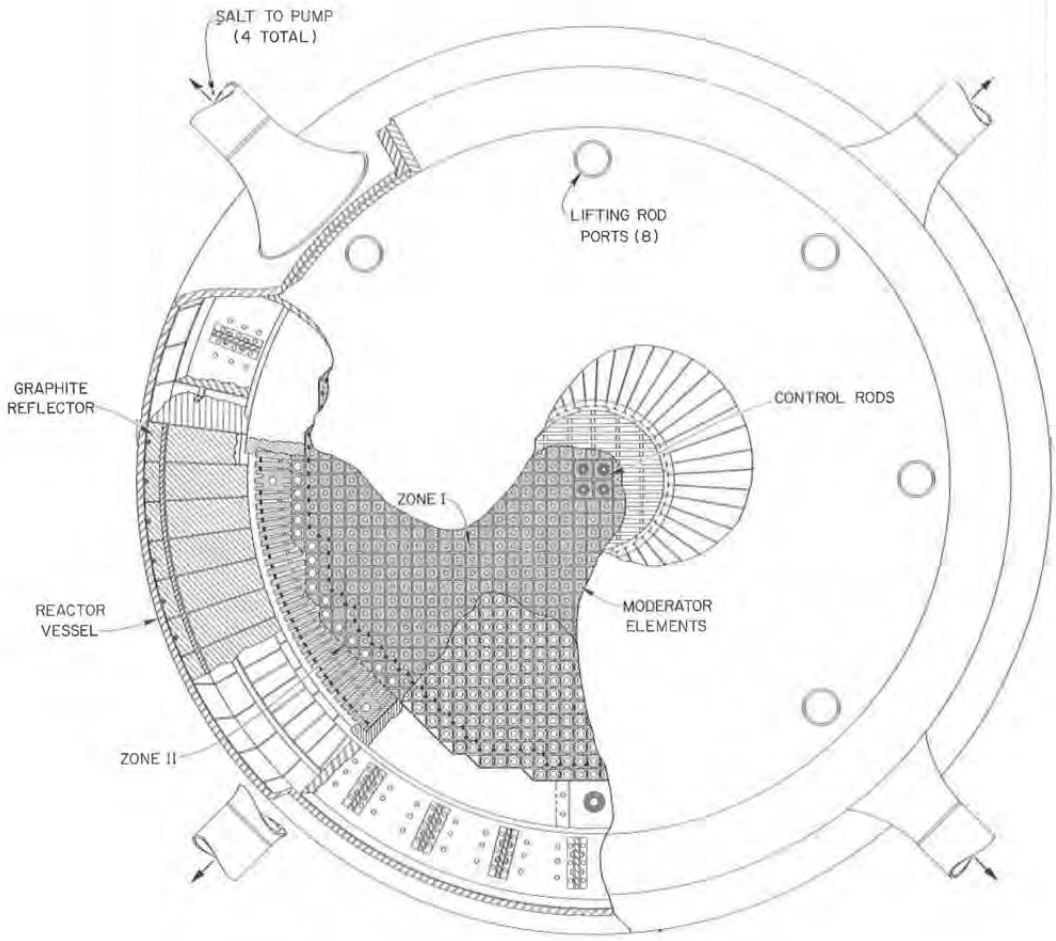
\includegraphics[height=1.05\textwidth]{./images/plan_view_vessel.png}
			\caption{Plan view of \gls{MSBR} vessel 
				\cite{robertson_conceptual_1971}.}
		\end{figure}
	\end{columns}
	
\end{textblock*}

\end{frame}


\begin{frame}
\frametitle{Geometry of MSBR model (Serpent)}

\begin{textblock*}{12.5cm}(0.1cm,1.9cm) % {block width} (coords)
\begin{figure}      
	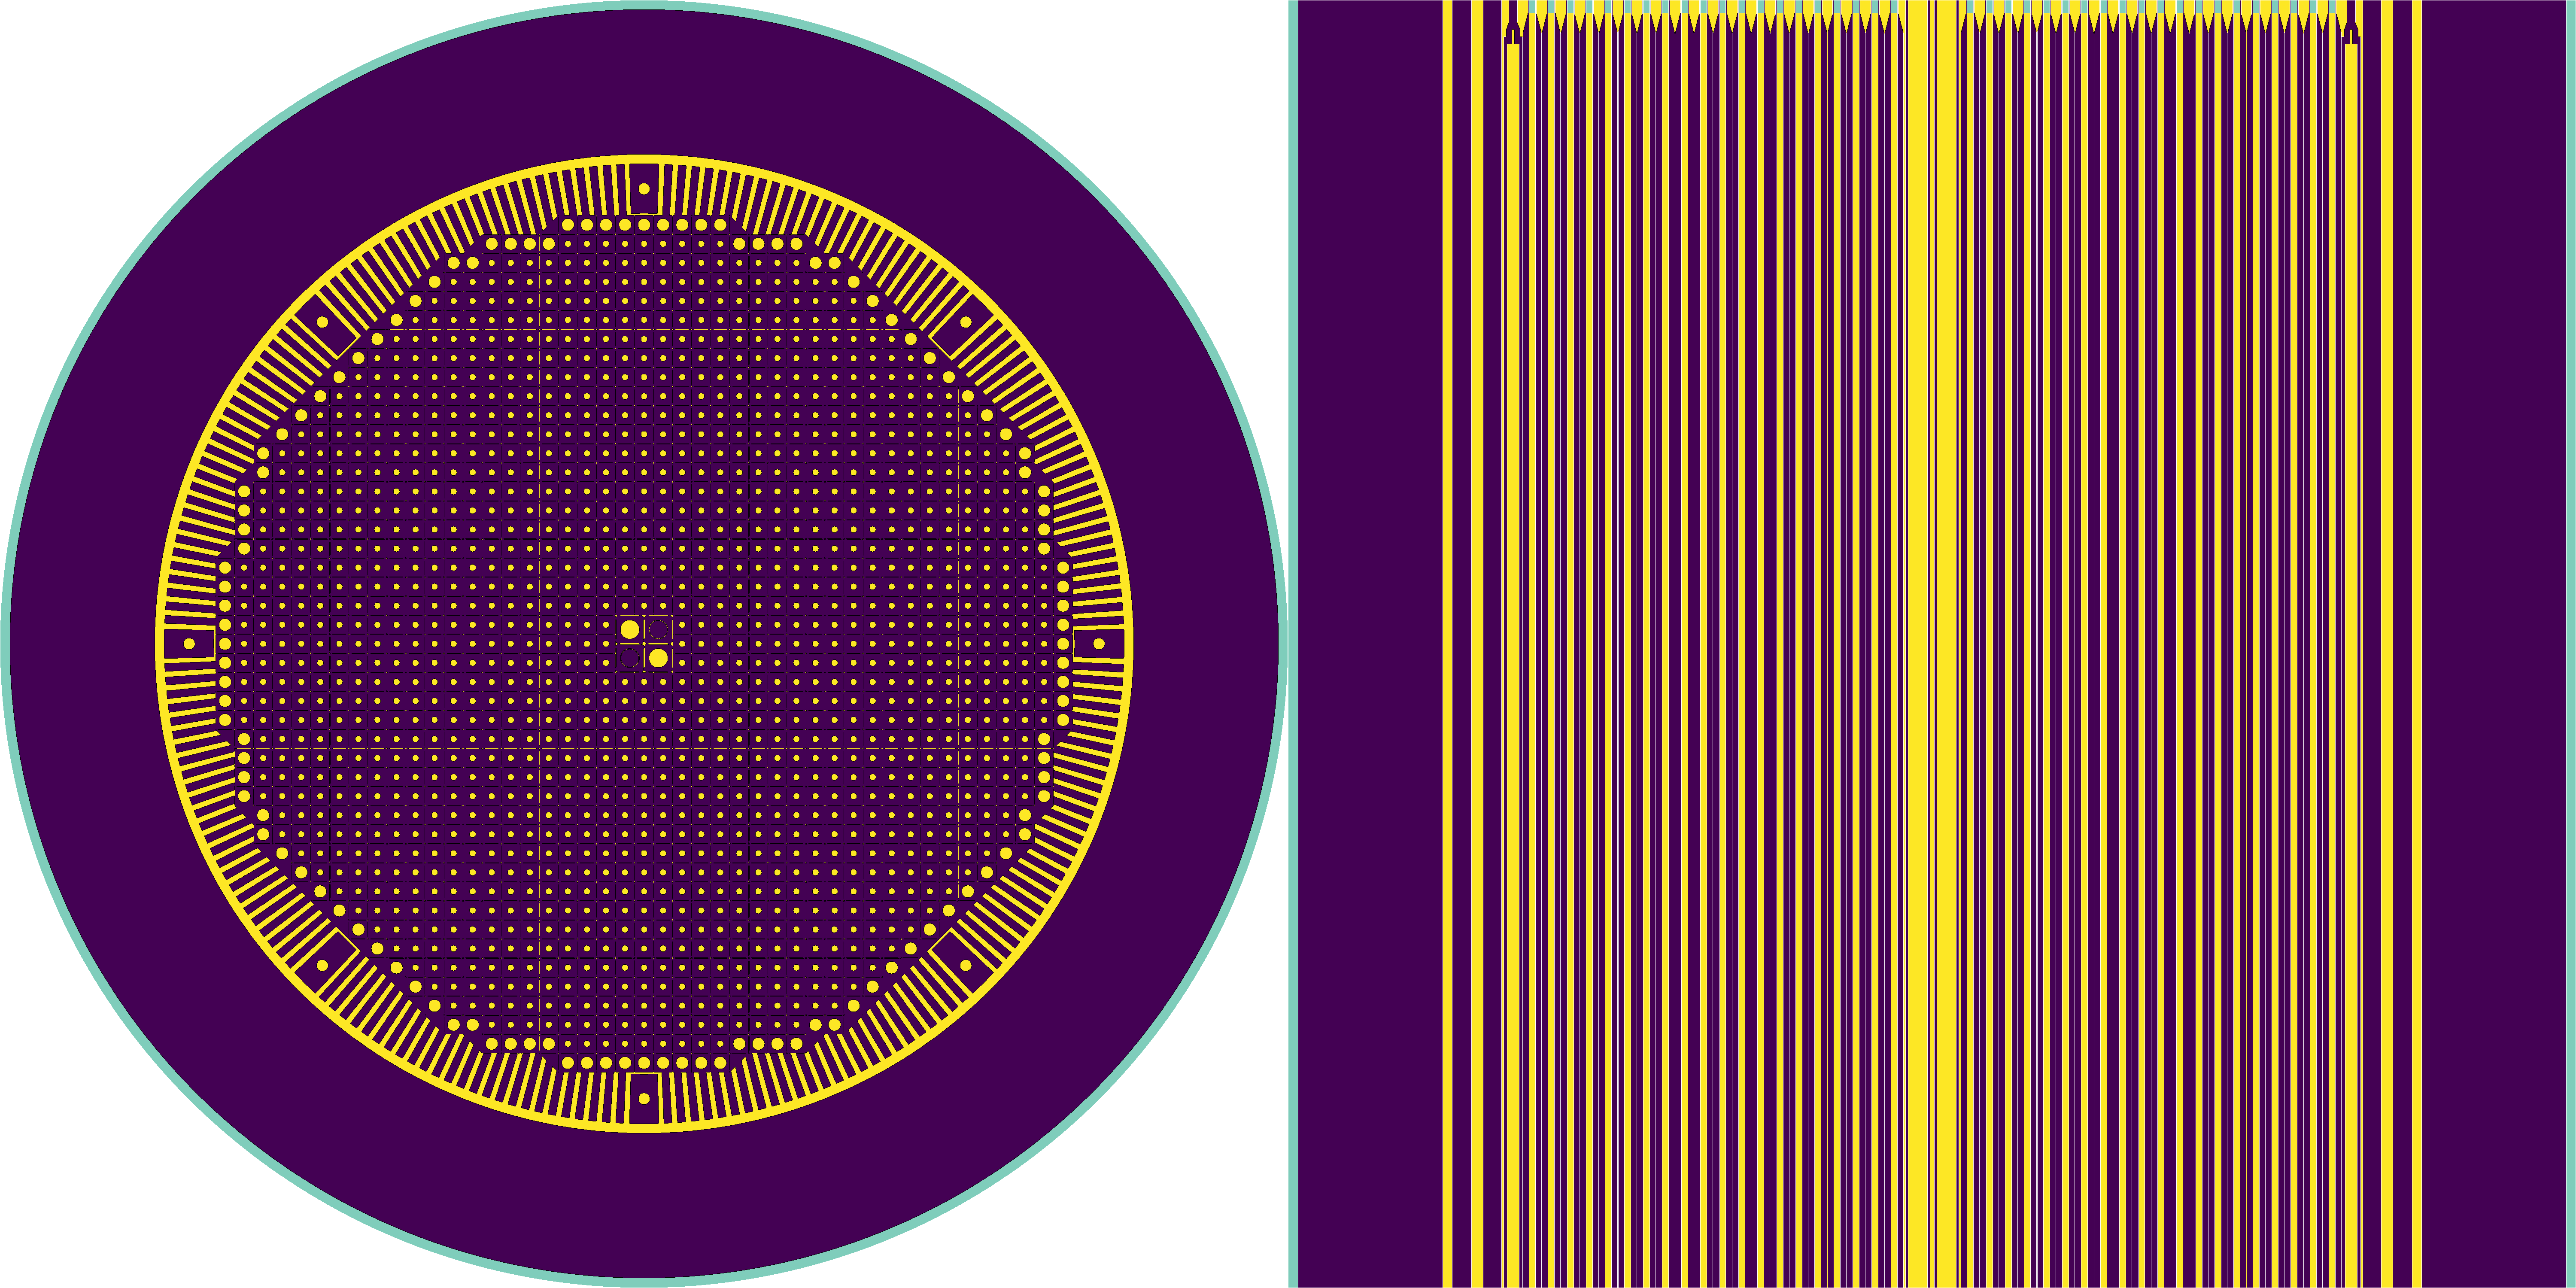
\includegraphics[width=\textwidth]{./images/geometry_main_views.png}
	\caption{An $XY$ (left) and $XZ$ (right) sections of \gls{MSBR} model. 
		The violet color represents graphite, the yellow - fuel salt 	
		\cite{rykhlevskii_full-core_2017}.}
\end{figure}
\end{textblock*}
\end{frame}

\begin{frame}
\frametitle{Moderator element geometry (Zone I)}
\begin{textblock*}{12.5cm}(0.1cm,1.9cm) % {block width} (coords)
\begin{figure}[t]
\includegraphics[width=\textwidth]{./images/zone_I_mesh.png}
\vspace{-5mm}
\caption{Molten Salt Breeder Reactor Zone I unit cell geometry from the 
	reference \cite{robertson_conceptual_1971} (left) and Serpent model 
	(right) \cite{rykhlevskii_full-core_2017}.}
\end{figure}
\end{textblock*}

\end{frame}

\begin{frame}
\frametitle{Graphite channels geometry}
\begin{textblock*}{12.5cm}(0.02cm,2.0cm) % {block width} (coords)
\begin{figure}[t]
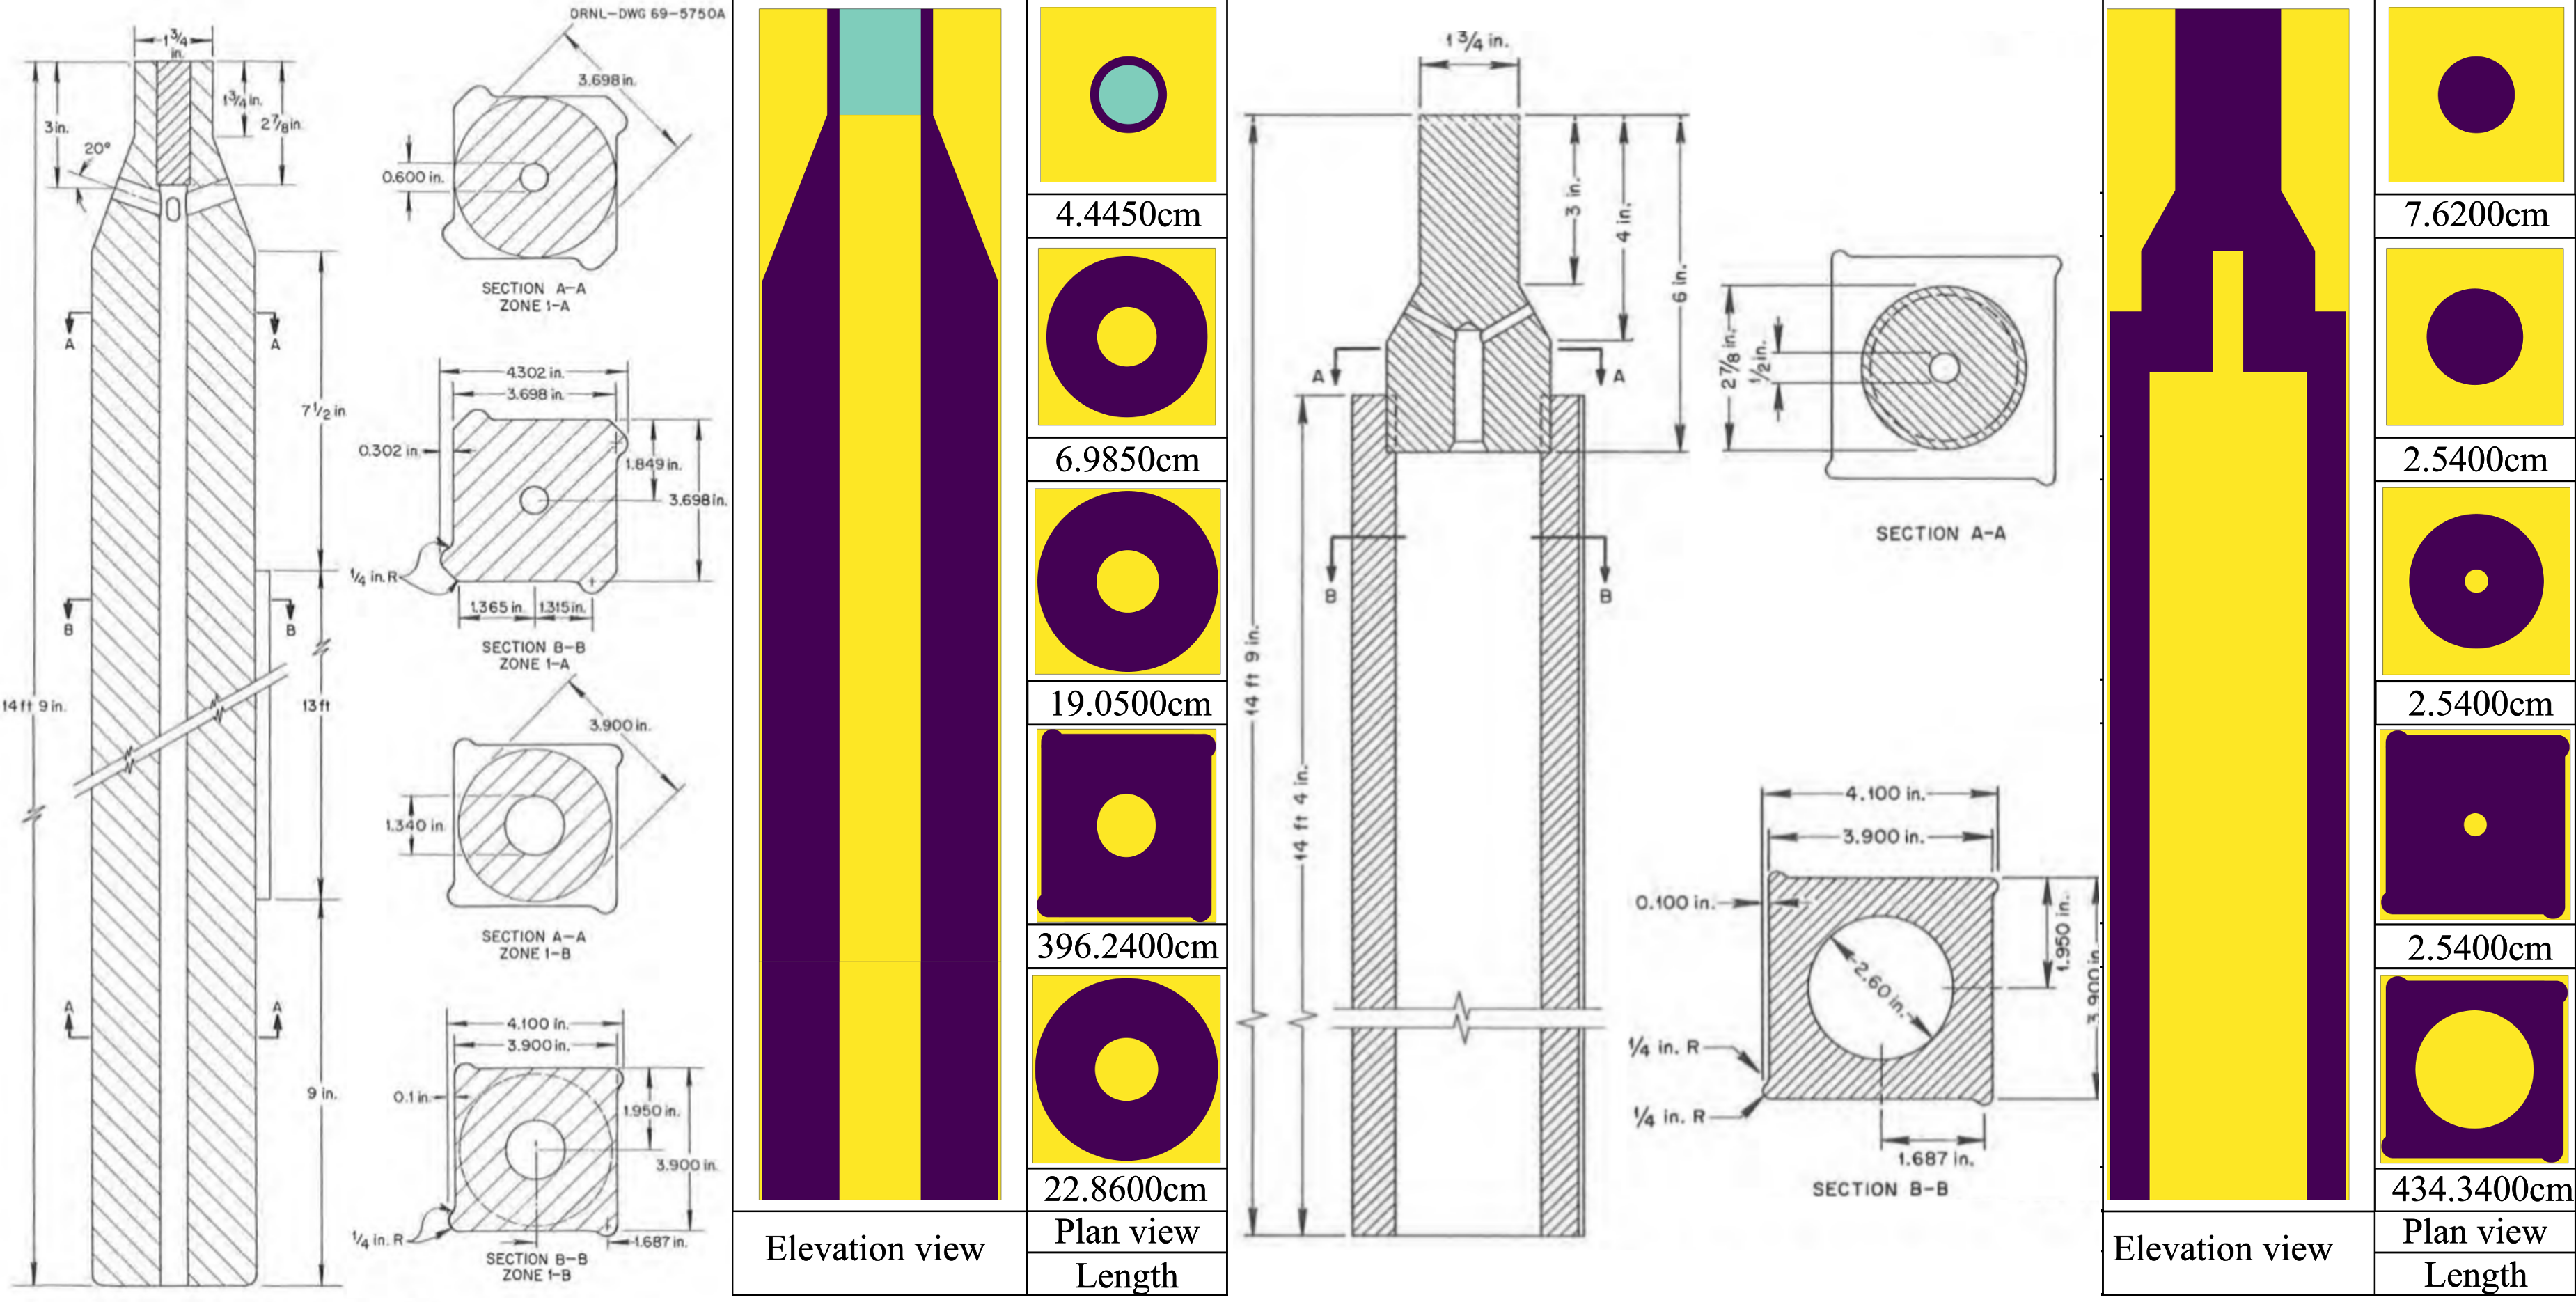
\includegraphics[width=1.02\textwidth]{./images/detailed_element_xz.png}
\vspace{-5mm}
\caption{Zone I (left) and Zone II (right) reference design 
\cite{robertson_conceptual_1971} and Serpent 
model \cite{rykhlevskii_full-core_2017}.}
\end{figure}
\end{textblock*}

\end{frame}


\begin{frame}
\frametitle{$k_{eff}$ dynamics during 60 years of MSBR operation}
\vspace{-3mm}
\begin{columns}
	\column{4.3cm}
	\begin{block}{Analysis assumptions}
		\fontsize{7}{9}\selectfont
		\begin{itemize}
			\item Full-core Serpent model
			\item Fine time resolution (\textbf{3-day} depletion step)
			\item Slowly extracted elements are removed at the end of the 
			cycle time (e.g., 50 days for RE)
			\item FP removal efficiency \textbf{fixed, ideal}
			\item All $^{233}$Pa removed and \textbf{equal mass of $^{233}$U} 
			fed to the core
			\item Fresh fertile material feed ($^{232}$Th) to maintain salt 
			inventory
		\end{itemize}
	\end{block}
	\vspace{-2mm}
	\begin{block}{Main findings}
	\fontsize{7}{9}\selectfont
	\begin{itemize}
		\item Strong absorbers ($^{234}$U) and fissile materials ($^{235}$U) 
		are built-up
		\item $k_{eff}$ stabilizes after $\approx6$ years
	\end{itemize}  
	\end{block}  	
	
	\column{8cm}
	\begin{figure}[ht!] 
	\begin{overprint}
	\onslide<1>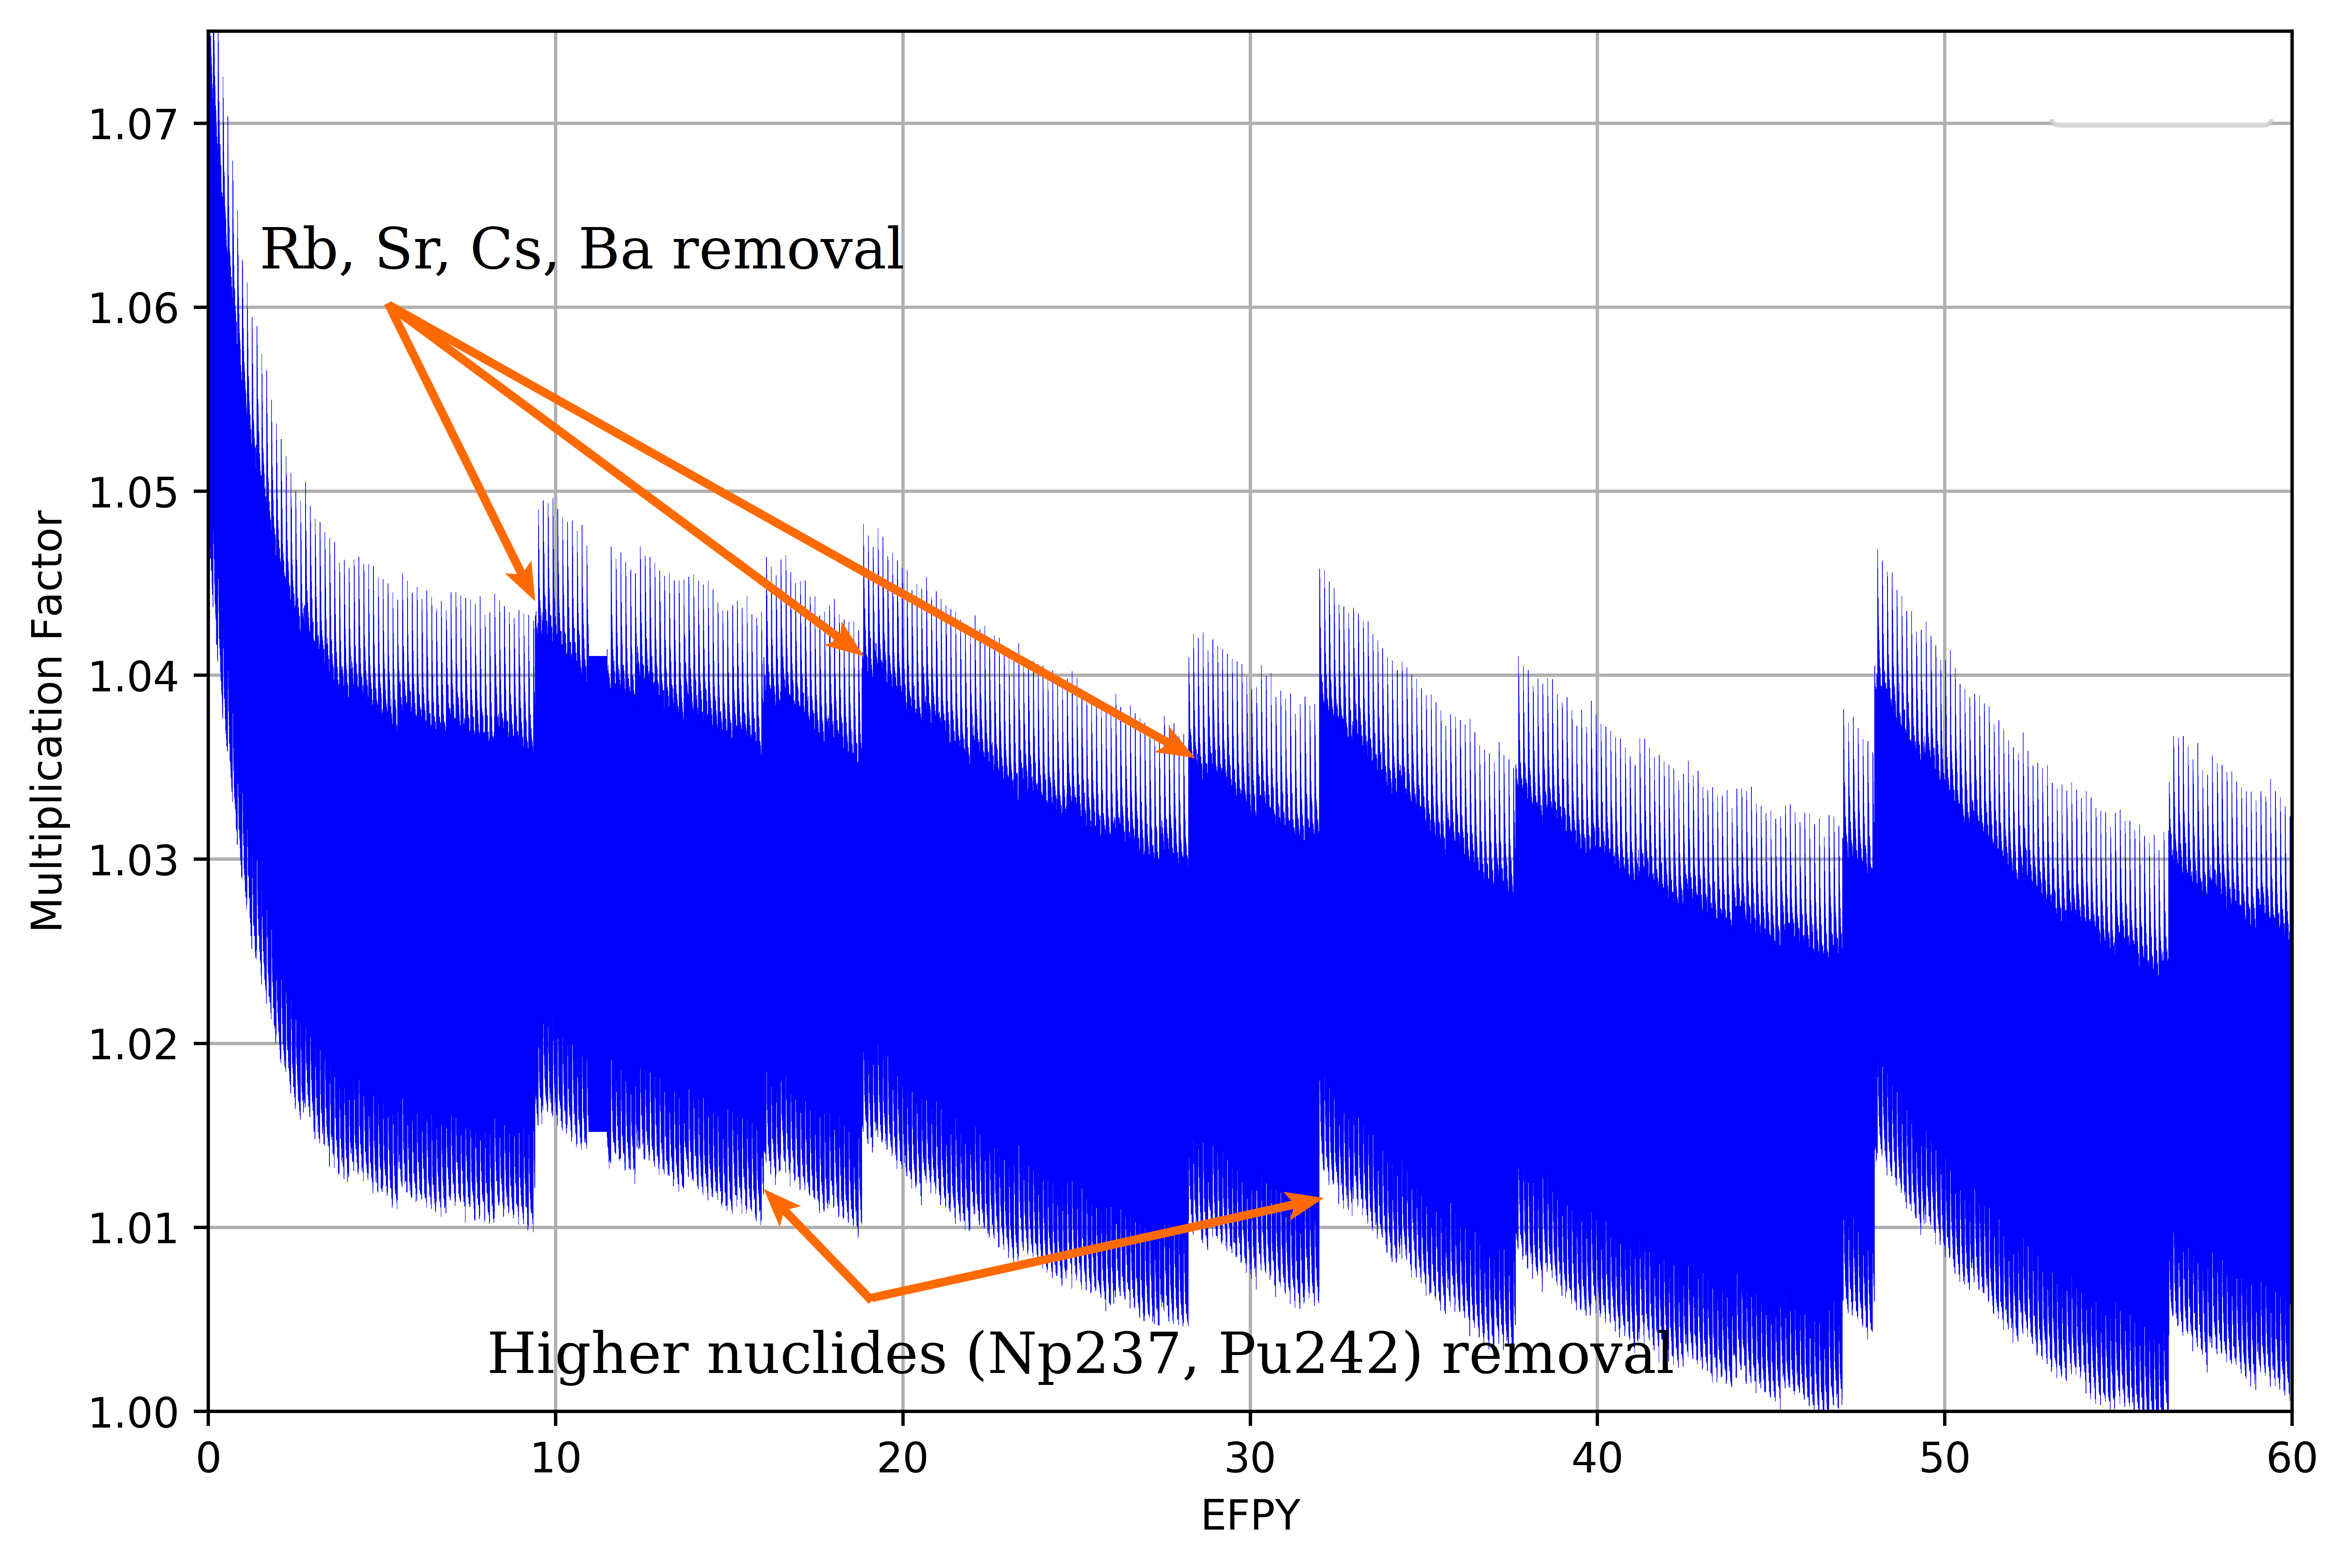
\includegraphics[width=\textwidth]{../dissertation/figures/ch3/keff.png}
	\vspace{-2mm}
	\caption{Effective multiplication factor dynamics for the full-core 
	\gls{MSBR} model \cite{rykhlevskii_modeling_2019}.}
	\onslide<2>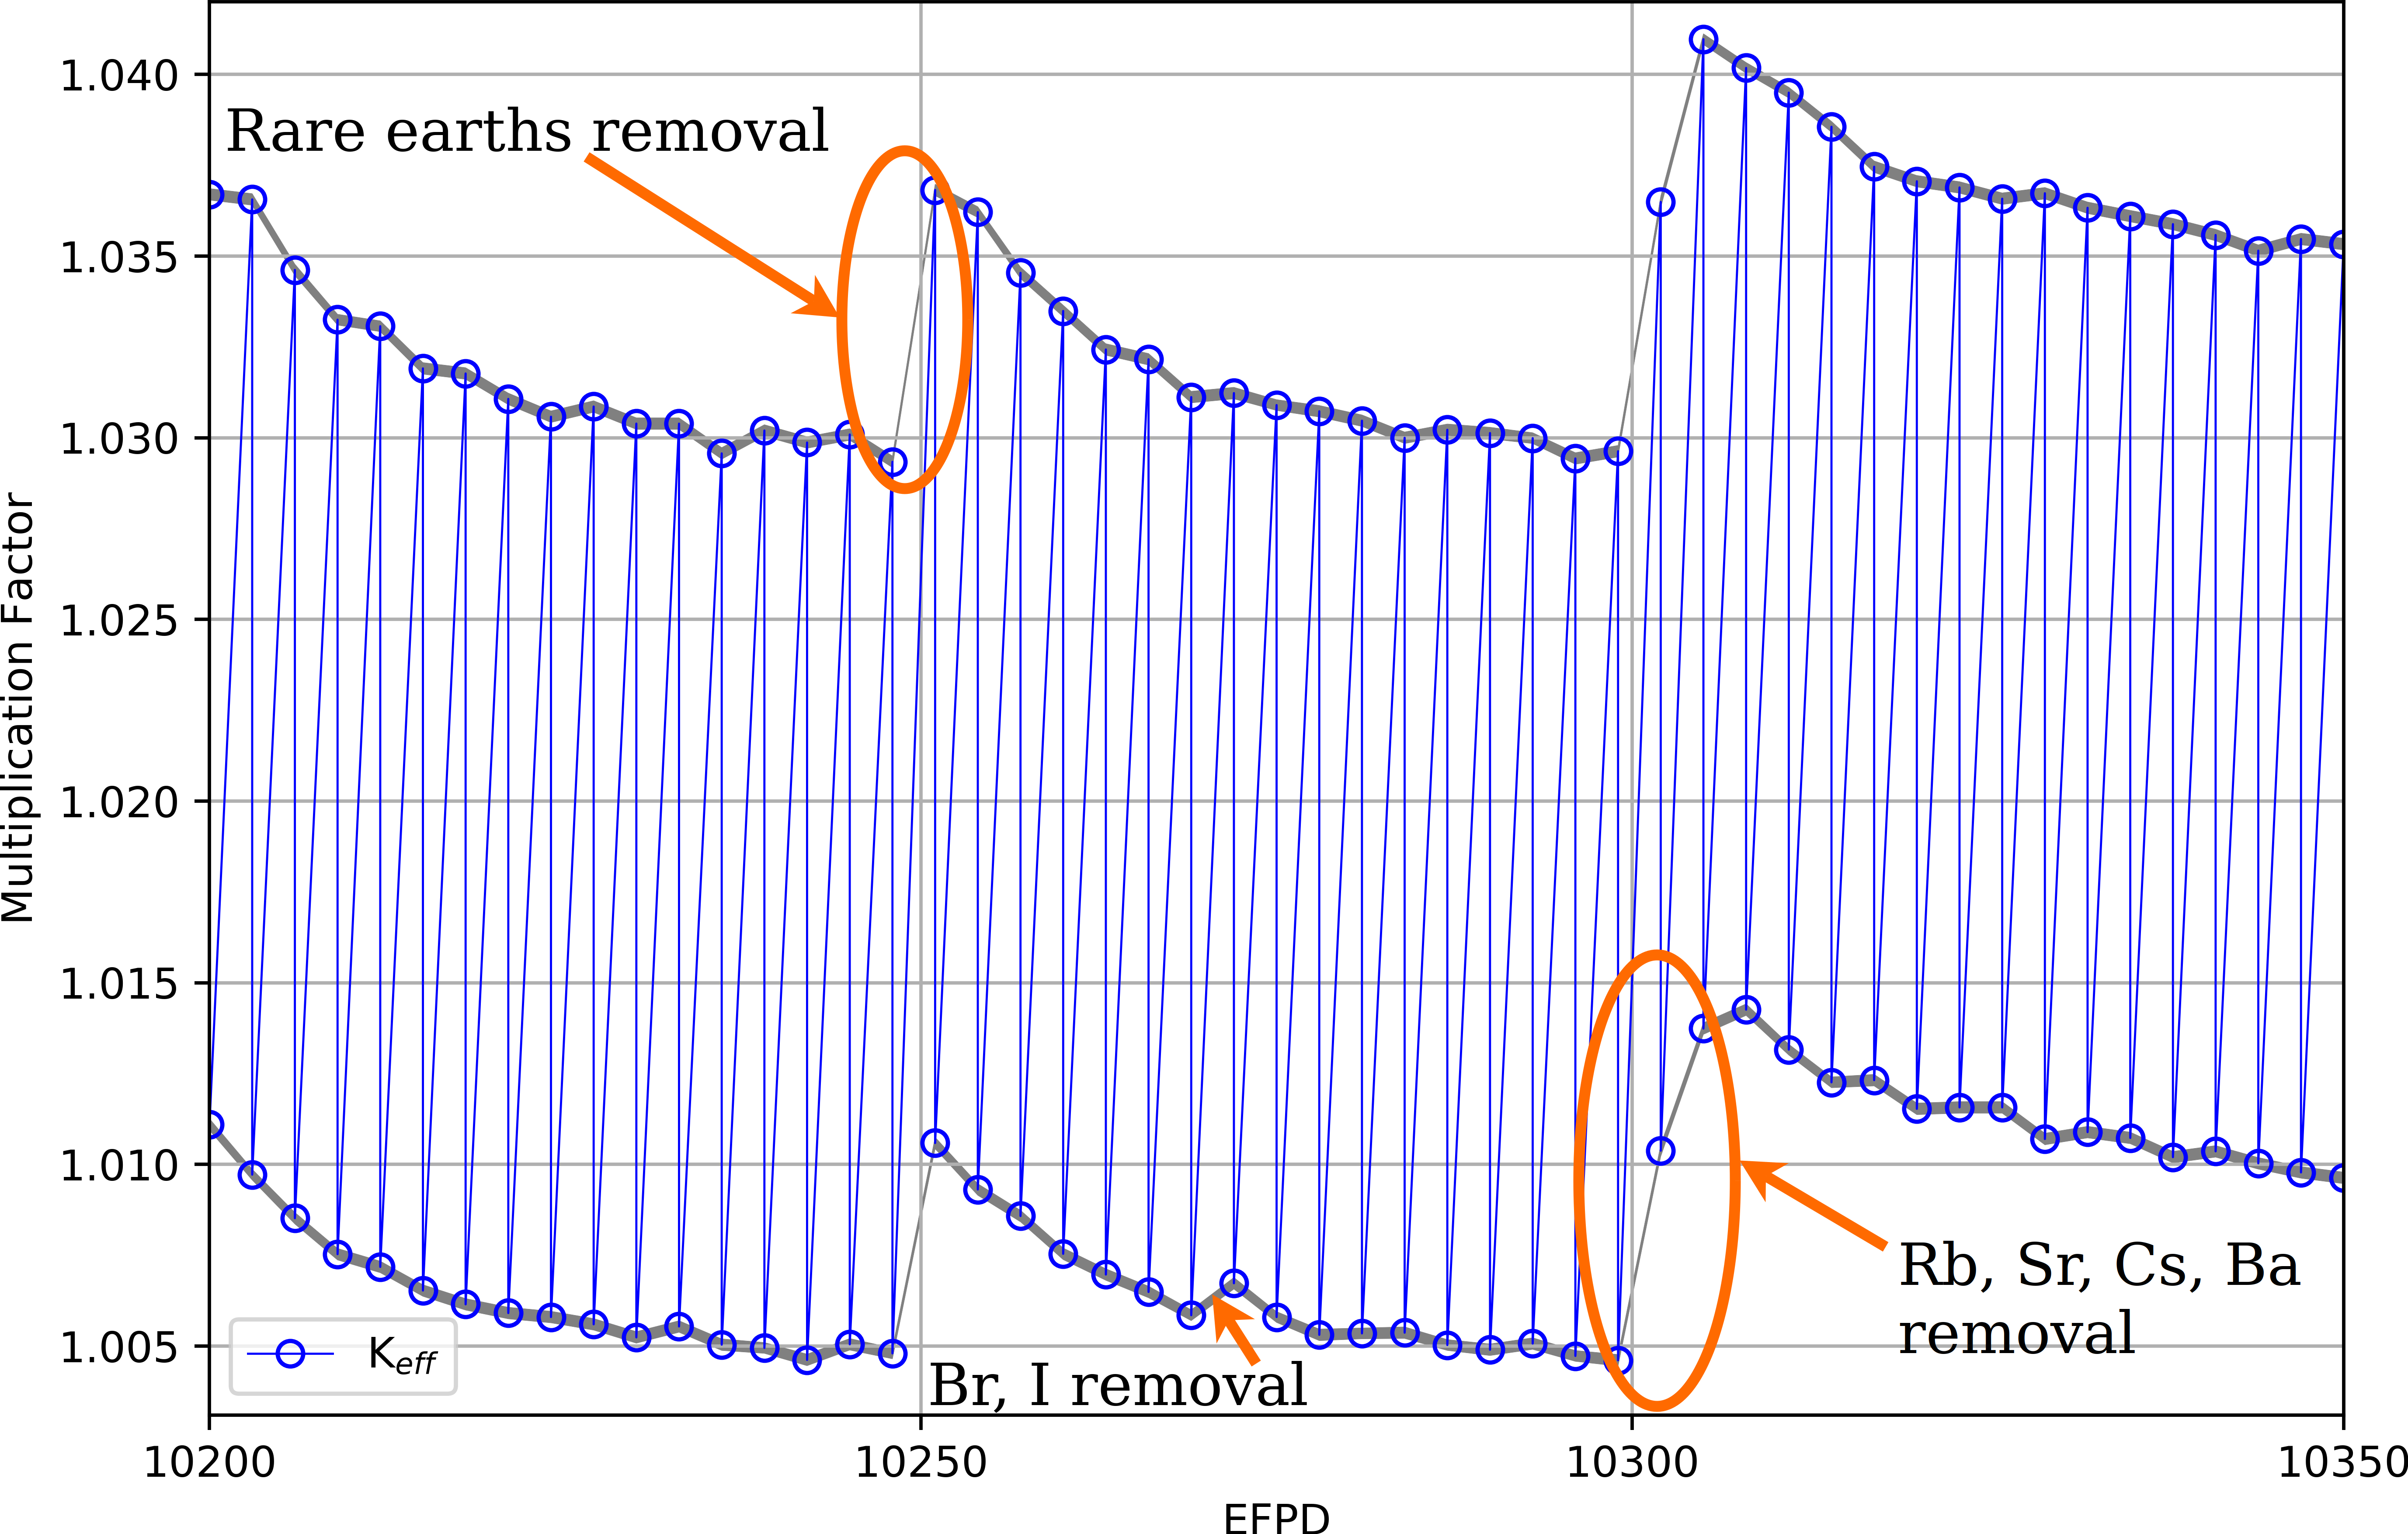
\includegraphics[width=\textwidth]{../dissertation/figures/ch3/keff_zoomed.png}
	\vspace{-0.5mm}
	\caption{\textbf{Zoomed} effective multiplication factor dynamics for the 
	full-core \gls{MSBR} model \cite{rykhlevskii_modeling_2019}.}
	\end{overprint}
	\end{figure}
	
\end{columns}
\end{frame}

\begin{frame}
\frametitle{Fuel salt composition evolution in the MSBR}
\begin{textblock*}{12.8cm}(0.03cm,2.6cm) % {block width} (coords)
\begin{columns}
	\column[t]{7cm}
	\vspace{-0.35in}
	\begin{figure}[t]
		\hspace{-5mm}
		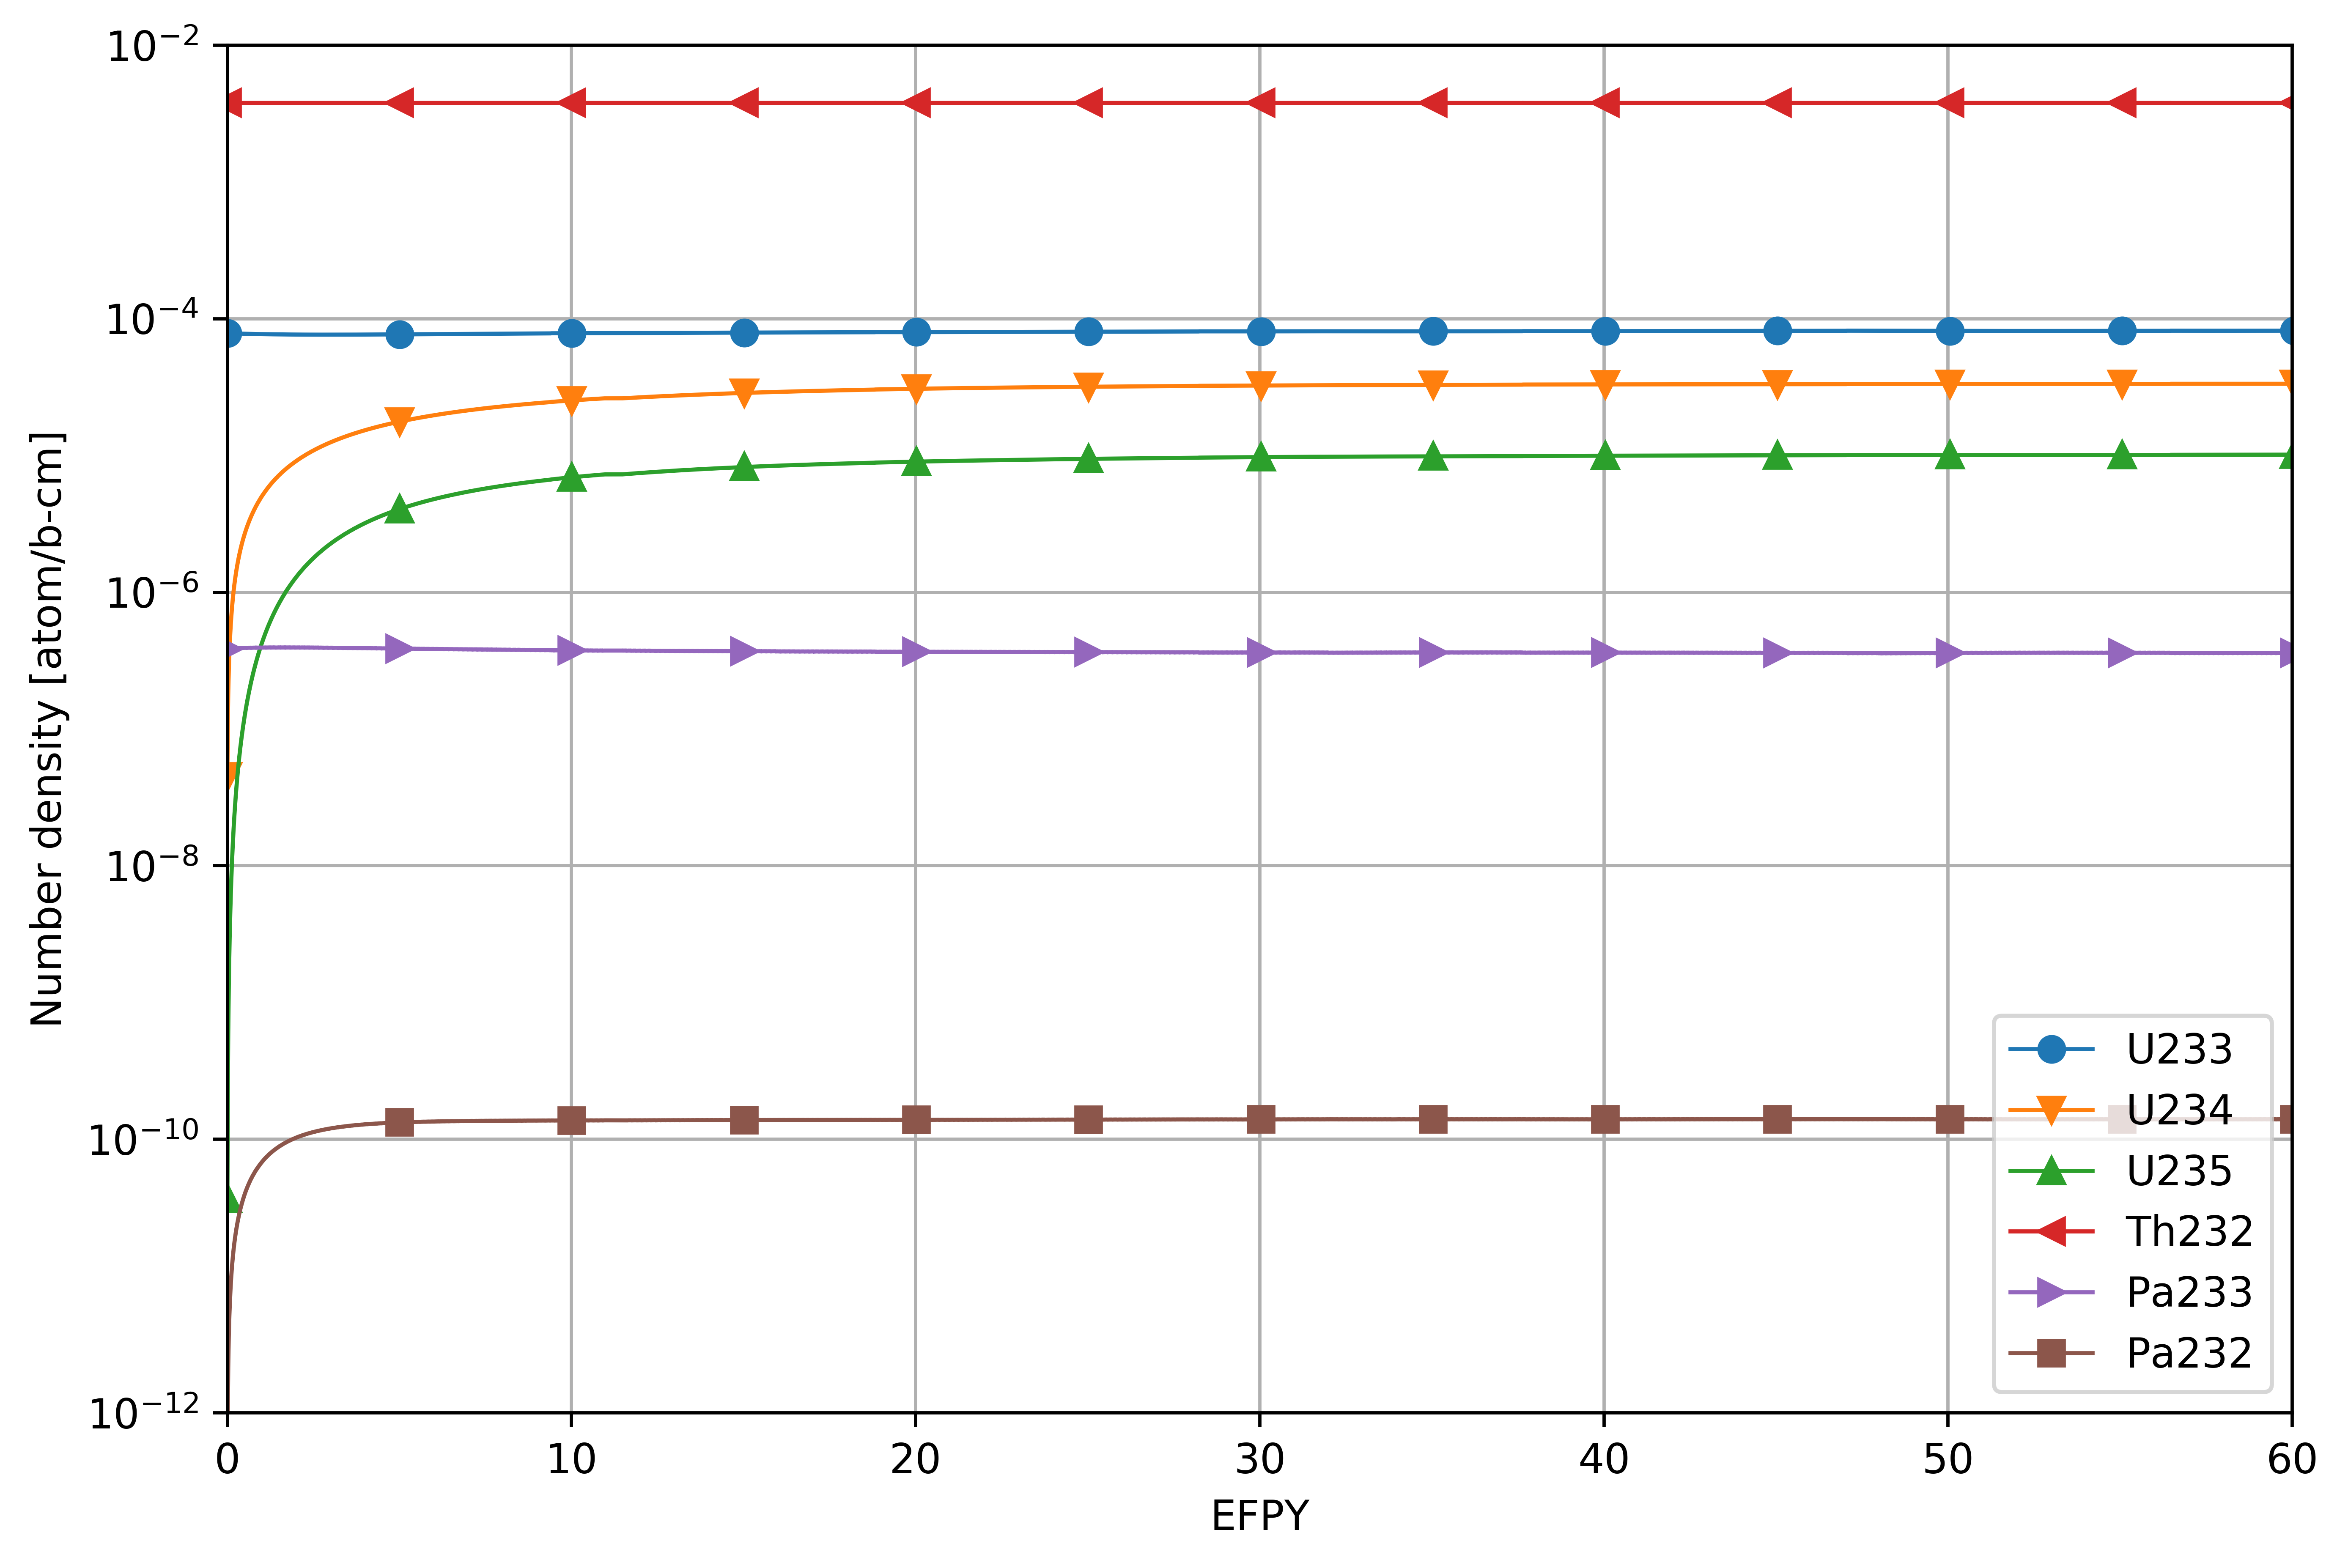
\includegraphics[height=0.69\textheight]{../dissertation/figures/ch3/major_isotopes_adens.png}
		\vspace{-0.15in}
		\caption{Normalized number density of major isotopes in the salt
			during 60 years of operation \cite{rykhlevskii_advanced_2018}.}
	\end{figure}
	
	\column[t]{4.5cm}
	\fontsize{7}{9}\selectfont
		\vspace{-3mm}
	\begin{itemize}
		\item<1-> Neutron poisons ($^{234}$U, $^{232}$Pa) accumulation has 
		negative impact on neutronics
		\item<1-> New fissile materials ($^{235}$U, $^{239}$Pu) improved core 
		performance
		\item<1-> $^{233}$U number density almost constant ($\Delta m<0.8\%$) 
		after 16 years of operation
		\item<1-> $^{242}$Th feed rate \textbf{2.4 kg/d is consistent with 
		ORNL results (2.45 kg/d) \cite{betzler_personal_2017}}
		\item<2-> Neutron spectrum \textbf{hardens toward EOL} causing:
		\setbeamerfont*{itemize/enumerate body}{size=\footnotesize}
		\setbeamerfont*{itemize/enumerate subbody}{parent=itemize/enumerate 
		body}
		\setbeamerfont*{itemize/enumerate subsubbody}{parent=itemize/enumerate 
		body}
		\begin{itemize}
			\item<3-> Reduced $^{233}$U breeding
			\item<4->Temperature coefficient ($\alpha_T$) weakened 
			from $-1.64$ to $-1.58pcm/K$
			\item<5->16\% decline in total control rod worth (CRW)
		\end{itemize} 
	\end{itemize}
\end{columns}
\end{textblock*}
\end{frame}


\begin{frame}
\frametitle{Effect of fission products removal}       

\begin{figure}[t] % replace 't' with 'b' to force it to 
	\centering
	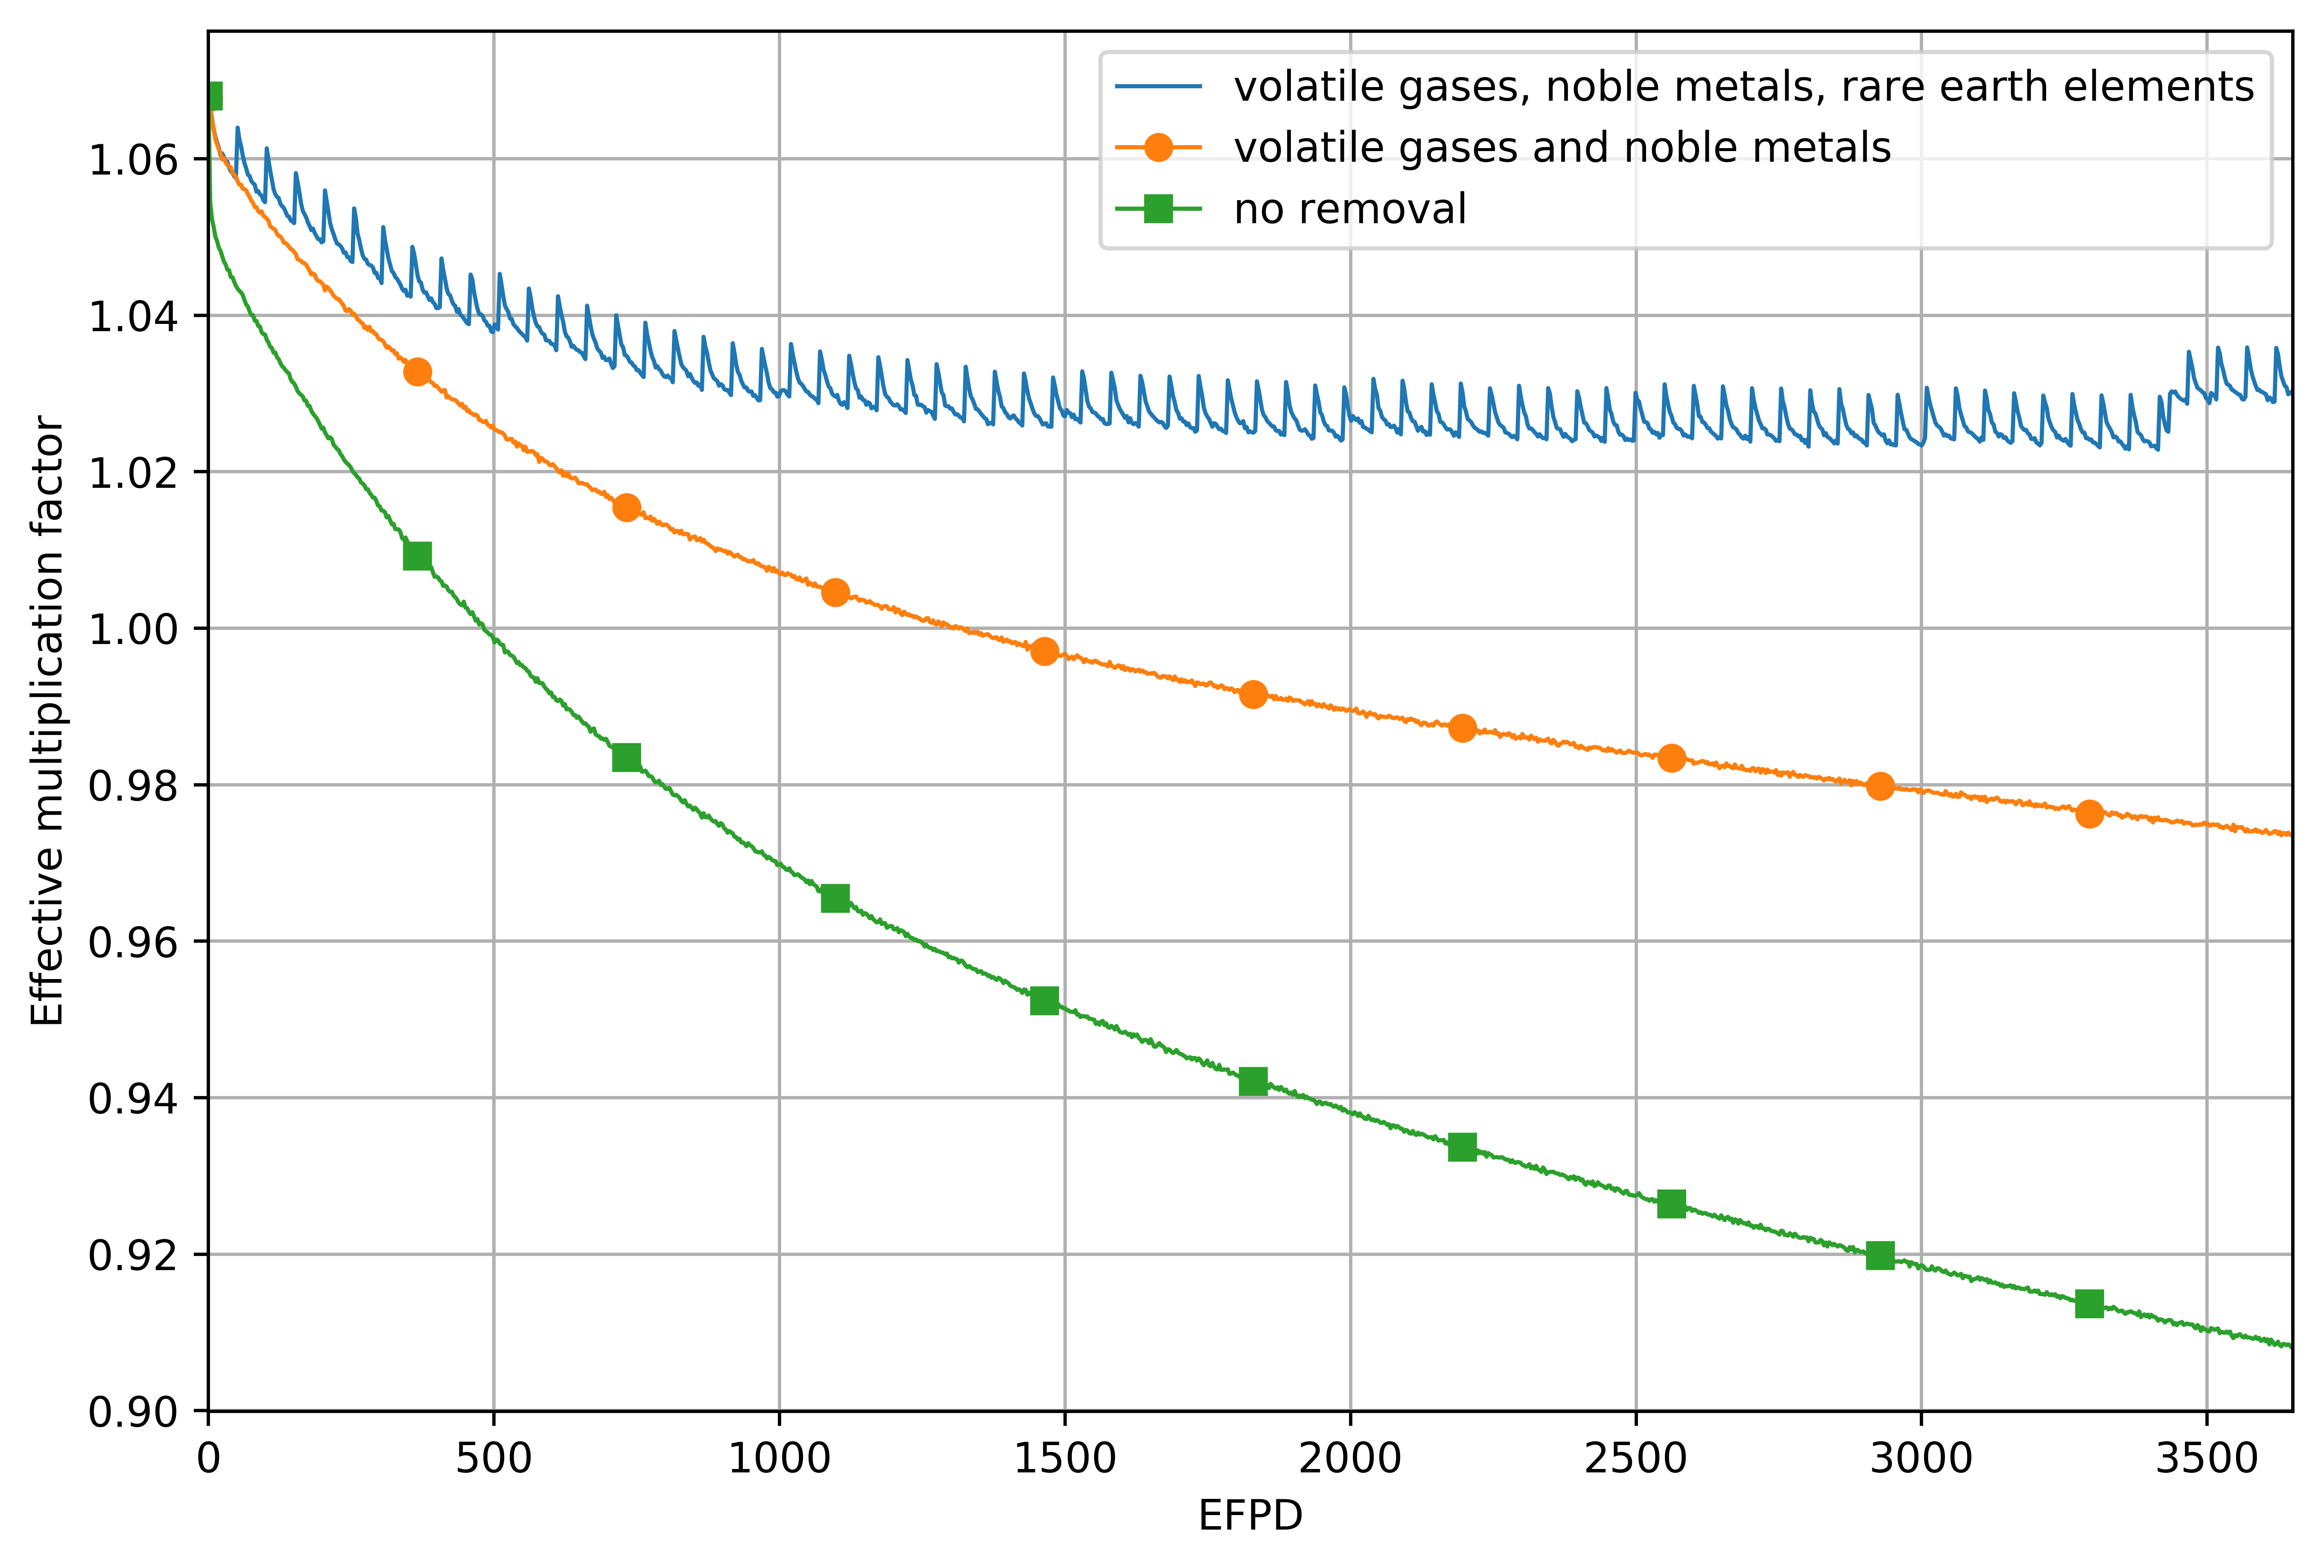
\includegraphics[width=0.9\textwidth]{../dissertation/figures/ch3/keff_rem_cases.png}
	 
		\vspace{-3mm}
	\caption{SaltProc-calculated effective multiplication factor for the 
	full-core \gls{MSBR} model with removal of various fission product groups 
	over 10	years of operation \cite{rykhlevskii_modeling_2019}.}
\end{figure}

\end{frame}



\subsection{Lifetime-long depletion: \gls{TAP} MSR}

\begin{frame}
\frametitle{TAP concept design}

\begin{textblock*}{12.7cm}(0.25cm,1.8cm) % {block width} (coords)
	
	\begin{columns}
		\column[t]{5cm}
		\vspace{+5mm}
		%%%%%%%%%%%%%%%%%%%%%%%%%%%%%%%%%%%%%%%%
		\begin{table}[h!]
			\fontsize{7}{9}\selectfont
			\caption{Summary of principal data
				\cite{transatomic_power_corporation_technical_2016}. }
			\vspace{-2mm}
			\begin{tabularx}{\textwidth}{ X  X }
				\hline
				Thermal power				           		& 1250 MW$_{th}  
				$       
				\\ 
				Electric power		                		& 520 MW$_e  
				$ 			 
				\\ 
				Gross thermal efficiency        			& 
				44\%     				 
				\\  
				Outlet temperature							& 
				620$^{\circ}$C         
				\\ 
				Fuel salt components                   & 
				LiF-UF$_4$				 \\  
				Fuel salt composition                  & 72.5-27.5 
				mole\%			 
				\\  
				Startup fissile material                     & 5\% 
				$^{235}$U          	 \\
				Moderator                              & ZrH$_{1.66}$ rods  \\
				Neutron spectrum						& 
				\textbf{thermal/epithermal}                 \\
				Moderator-to-fuel ratio						& 
				\textbf{varies in (0.1099, 1.0)}                 \\
				\hline
			\end{tabularx}
			\label{tab:tap_tab}
		\end{table}
		%%%%%%%%%%%%%%%%%%%%%%%%%%%%%%%%%%%%%%%%%%%%%%%%
		
		\column[t]{6.5cm}
		\hspace{-9mm}
		\begin{figure}      
			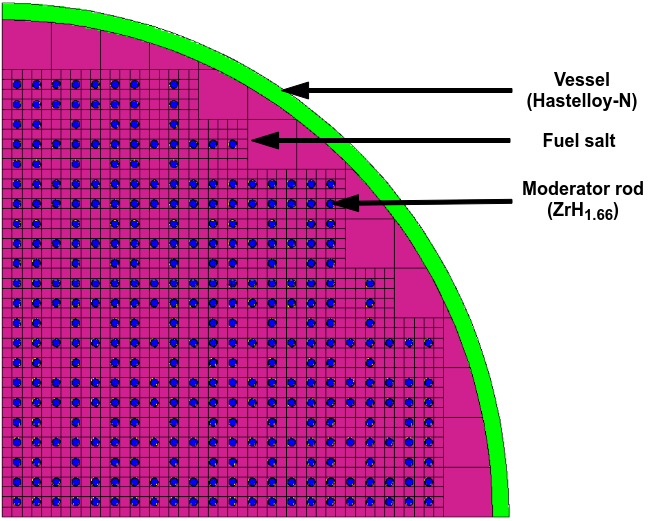
\includegraphics[height=0.79\textwidth]{../dissertation/figures/ch4/tap_core_ornl.png}
			\caption{The \gls{TAP} \gls{MSR} schematic core view showing 
				moderator rods configuration at \gls{BOL} 
				\cite{betzler_assessment_2017-1}.}
		\end{figure}
	\end{columns}
	
\end{textblock*}

\end{frame}

\begin{frame}
\frametitle{\gls{TAP} concept full-core high-fidelity Serpent model}
\begin{textblock*}{12.6cm}(0.1cm,1.8cm) % {block width} (coords)
\begin{figure}[htp!] % replace 't' with 'b' to 
	\begin{overprint}
		\onslide<1>\centerline{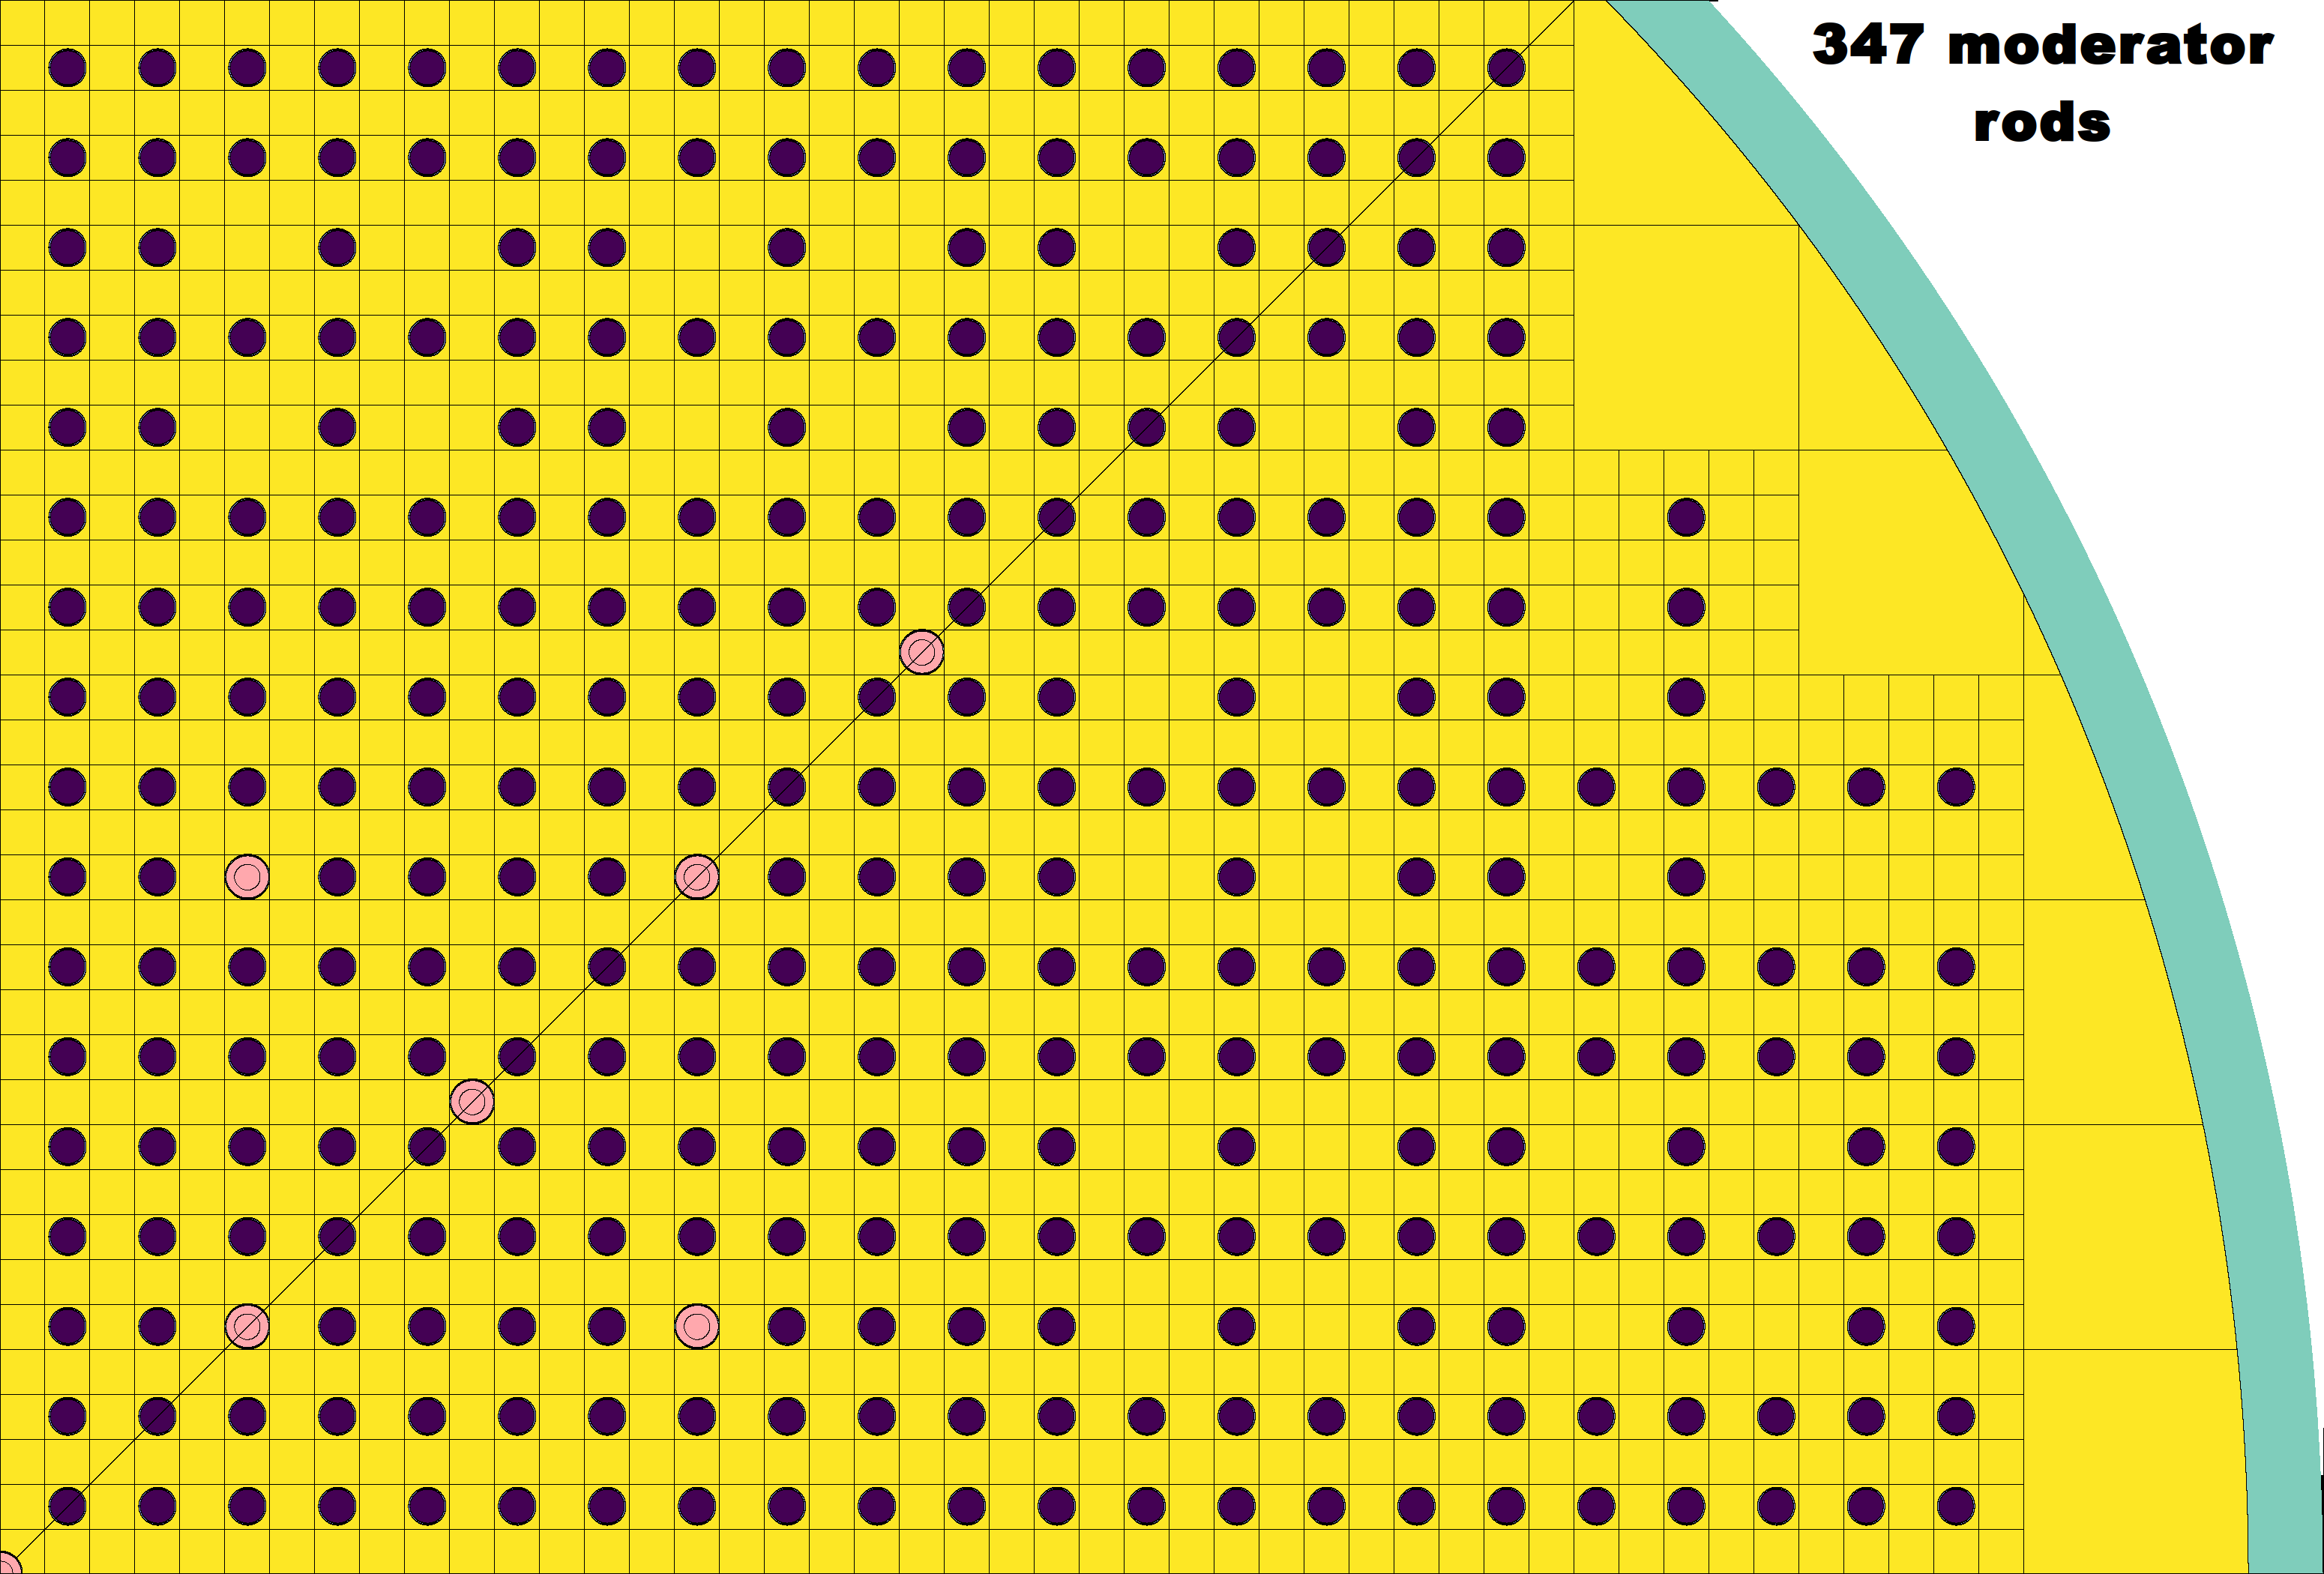
\includegraphics[height=0.75\textheight]{./images/347_base.png}}
		\onslide<2>\centerline{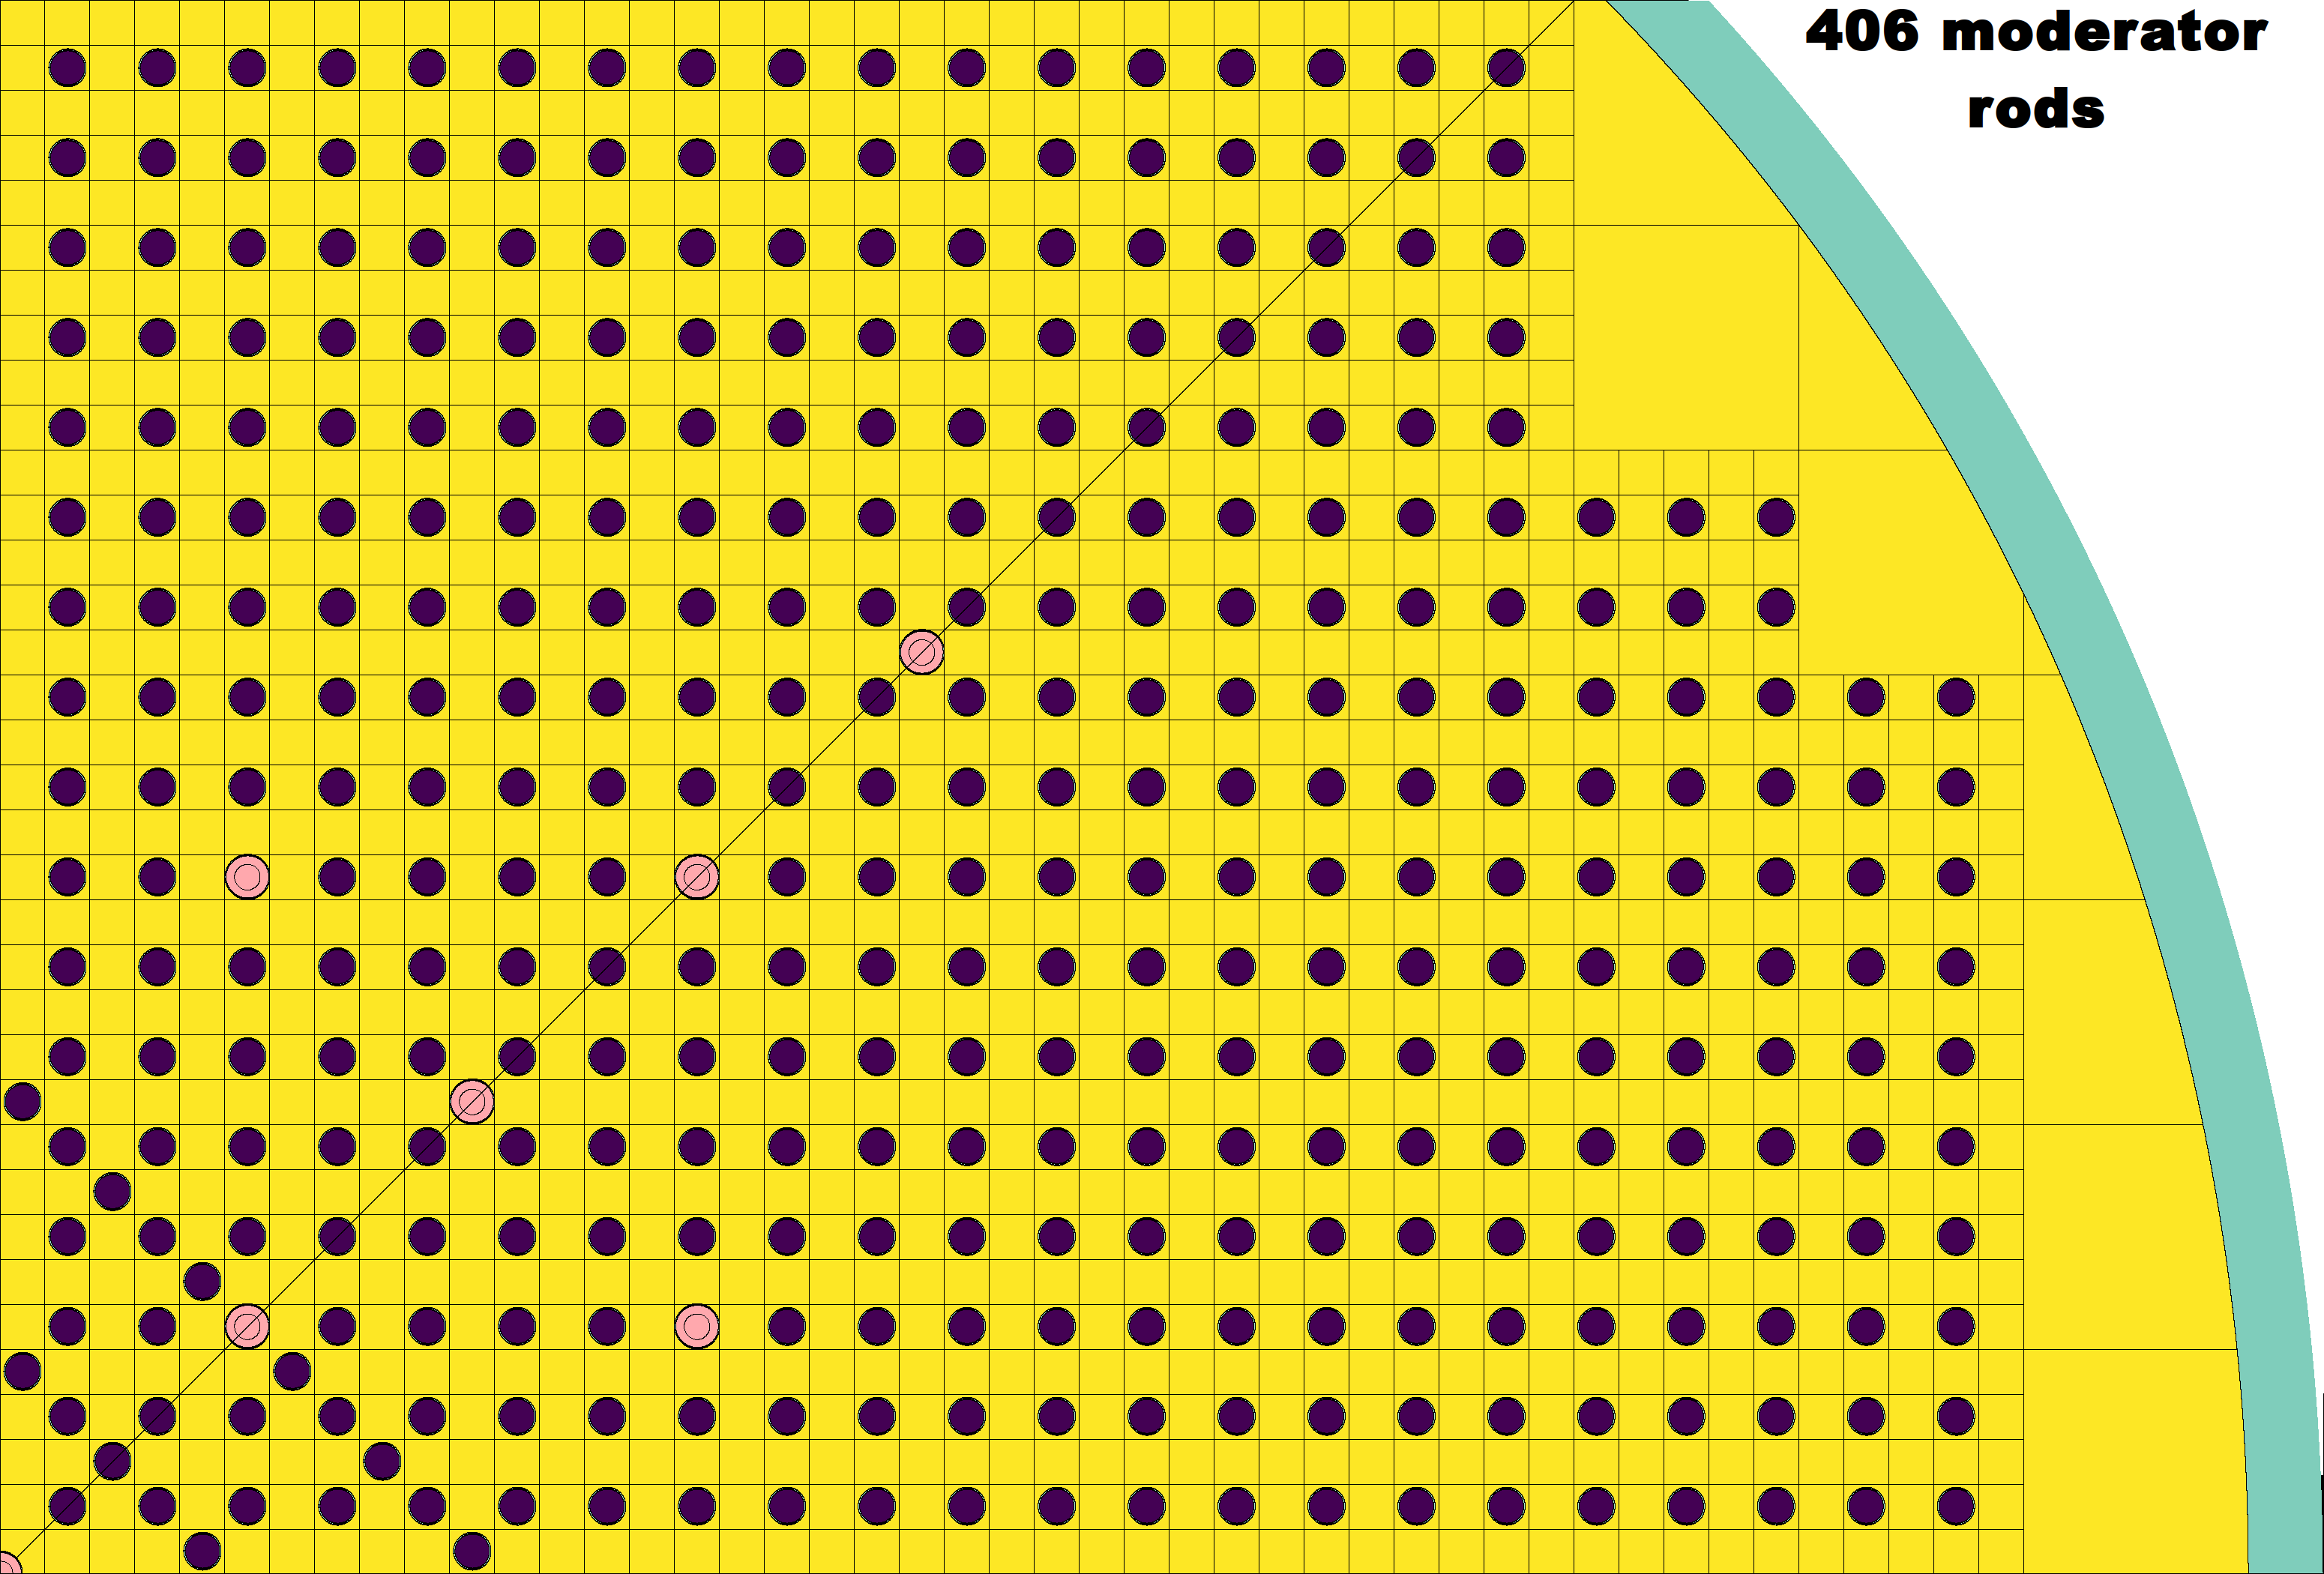
\includegraphics[height=0.75\textheight]{./images/406.png}}
		\onslide<3>\centerline{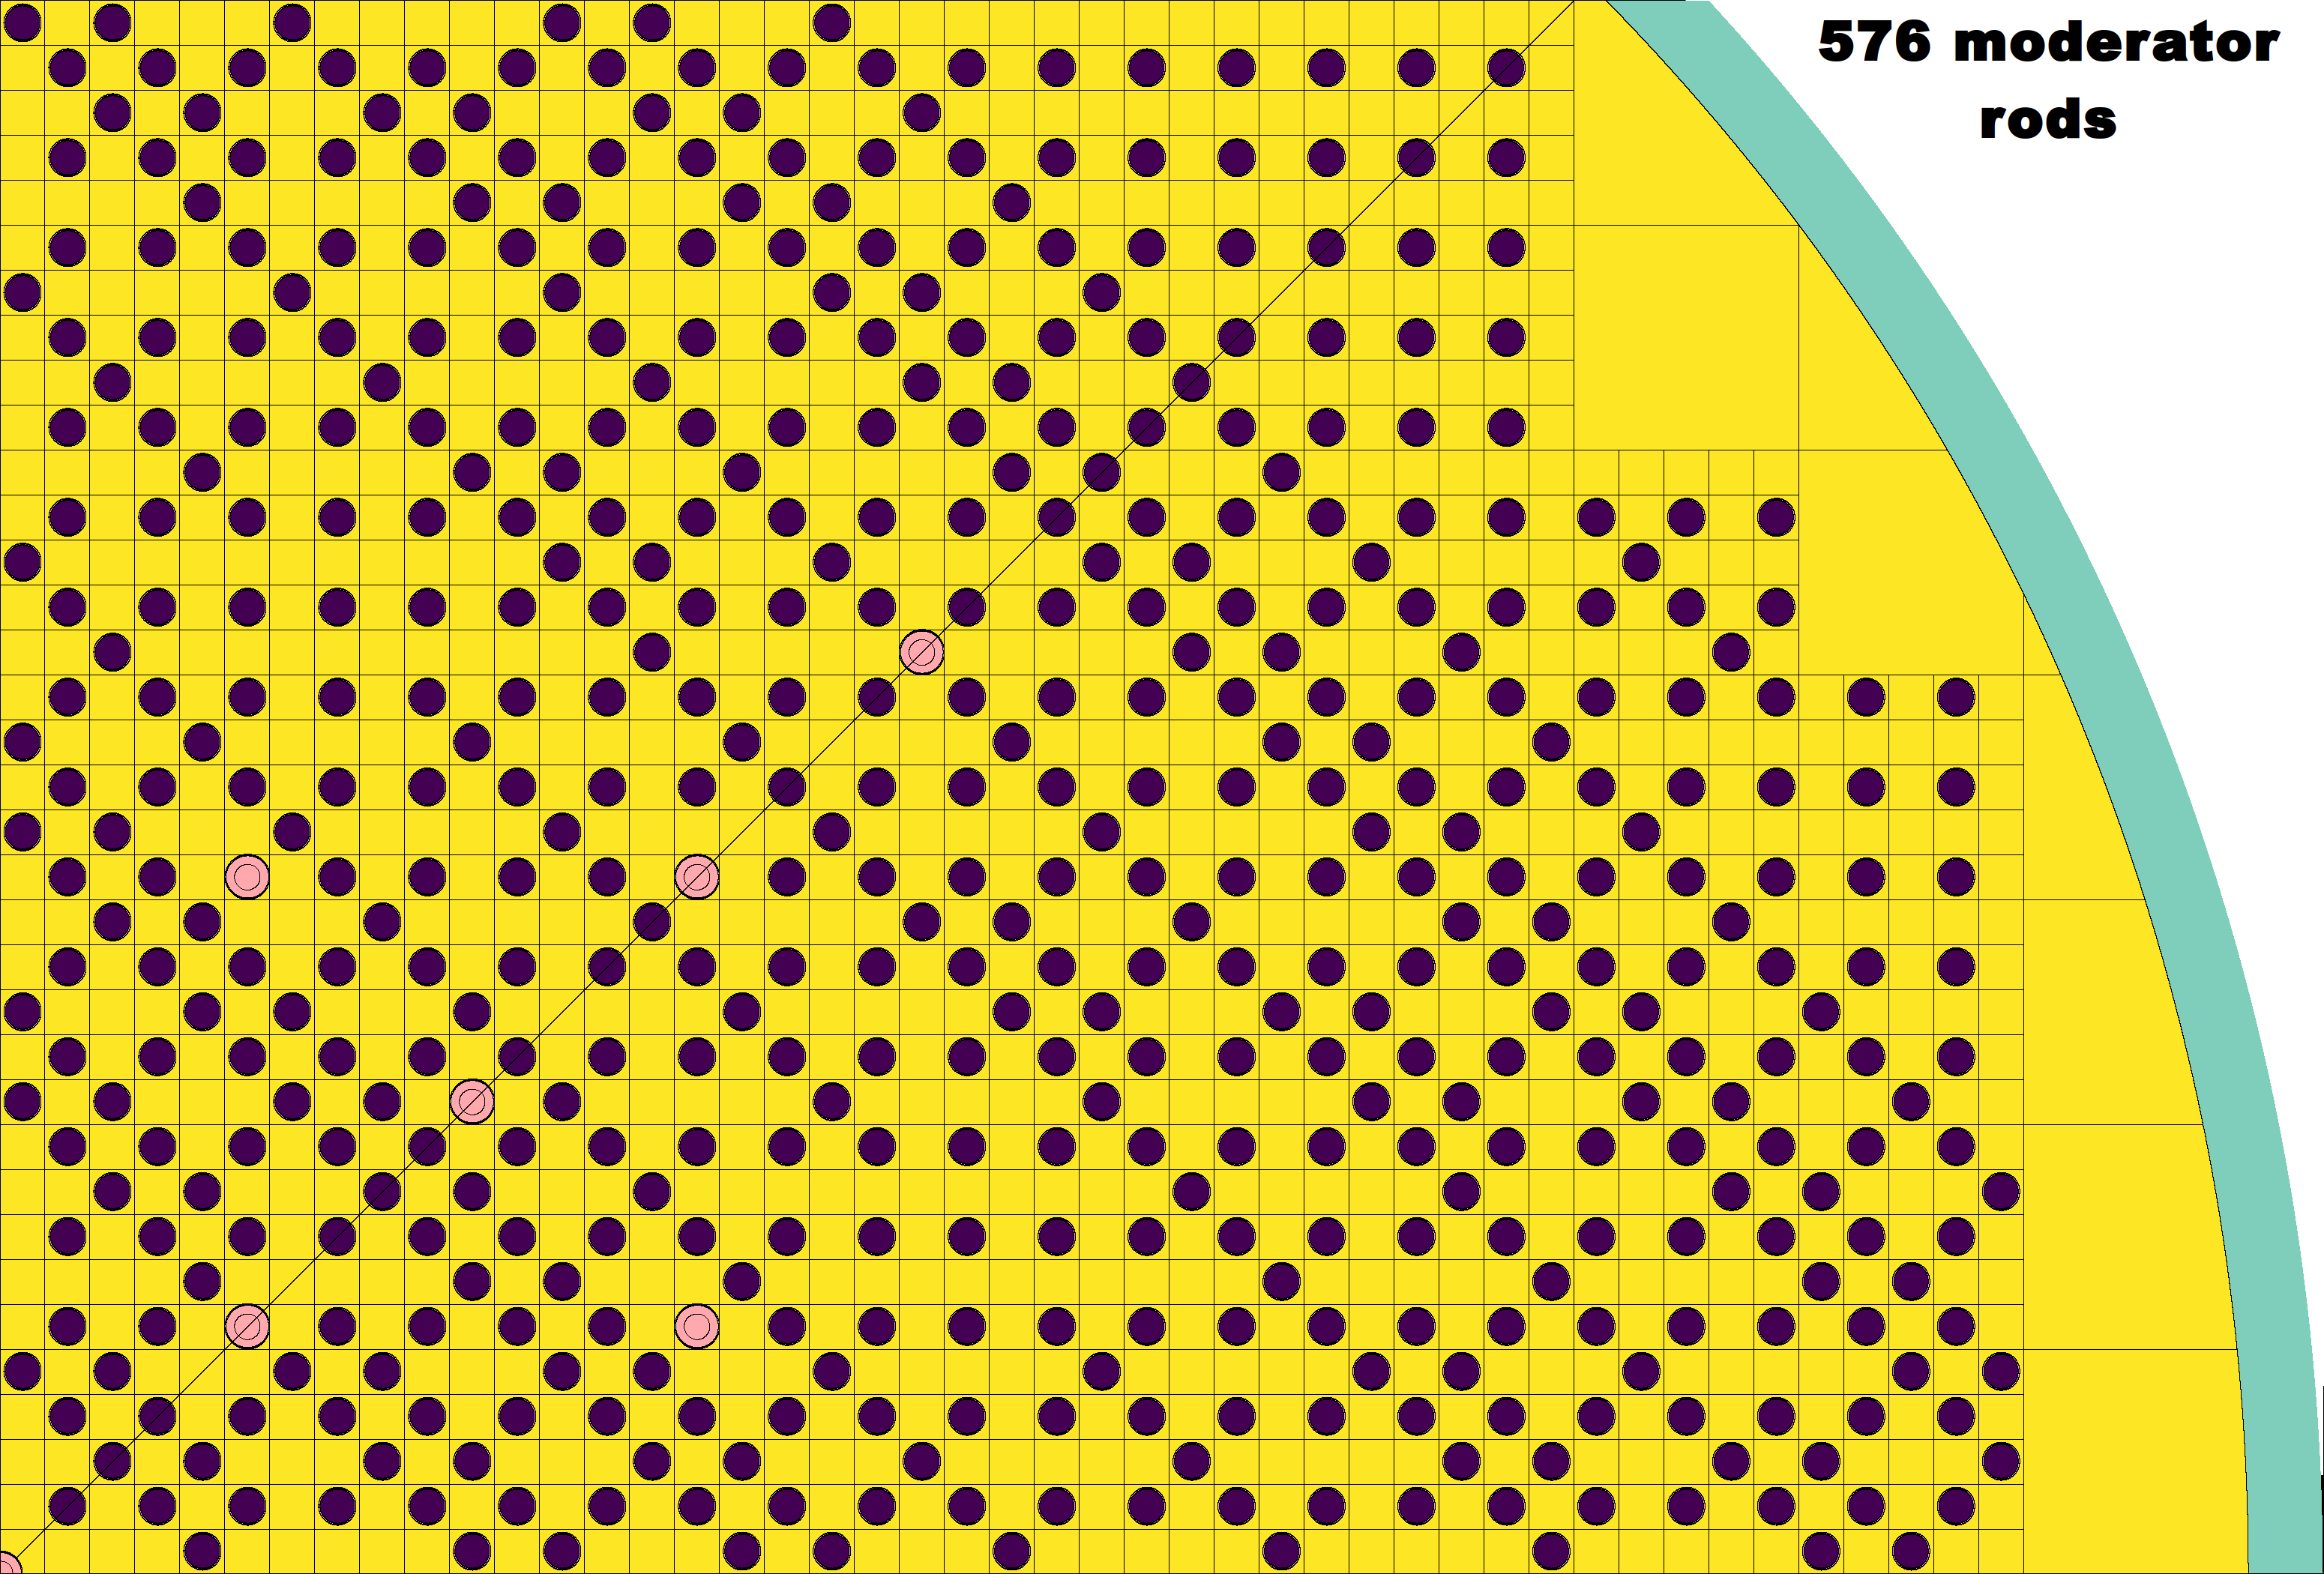
\includegraphics[height=0.75\textheight]{./images/576.png}}
		\onslide<4>\centerline{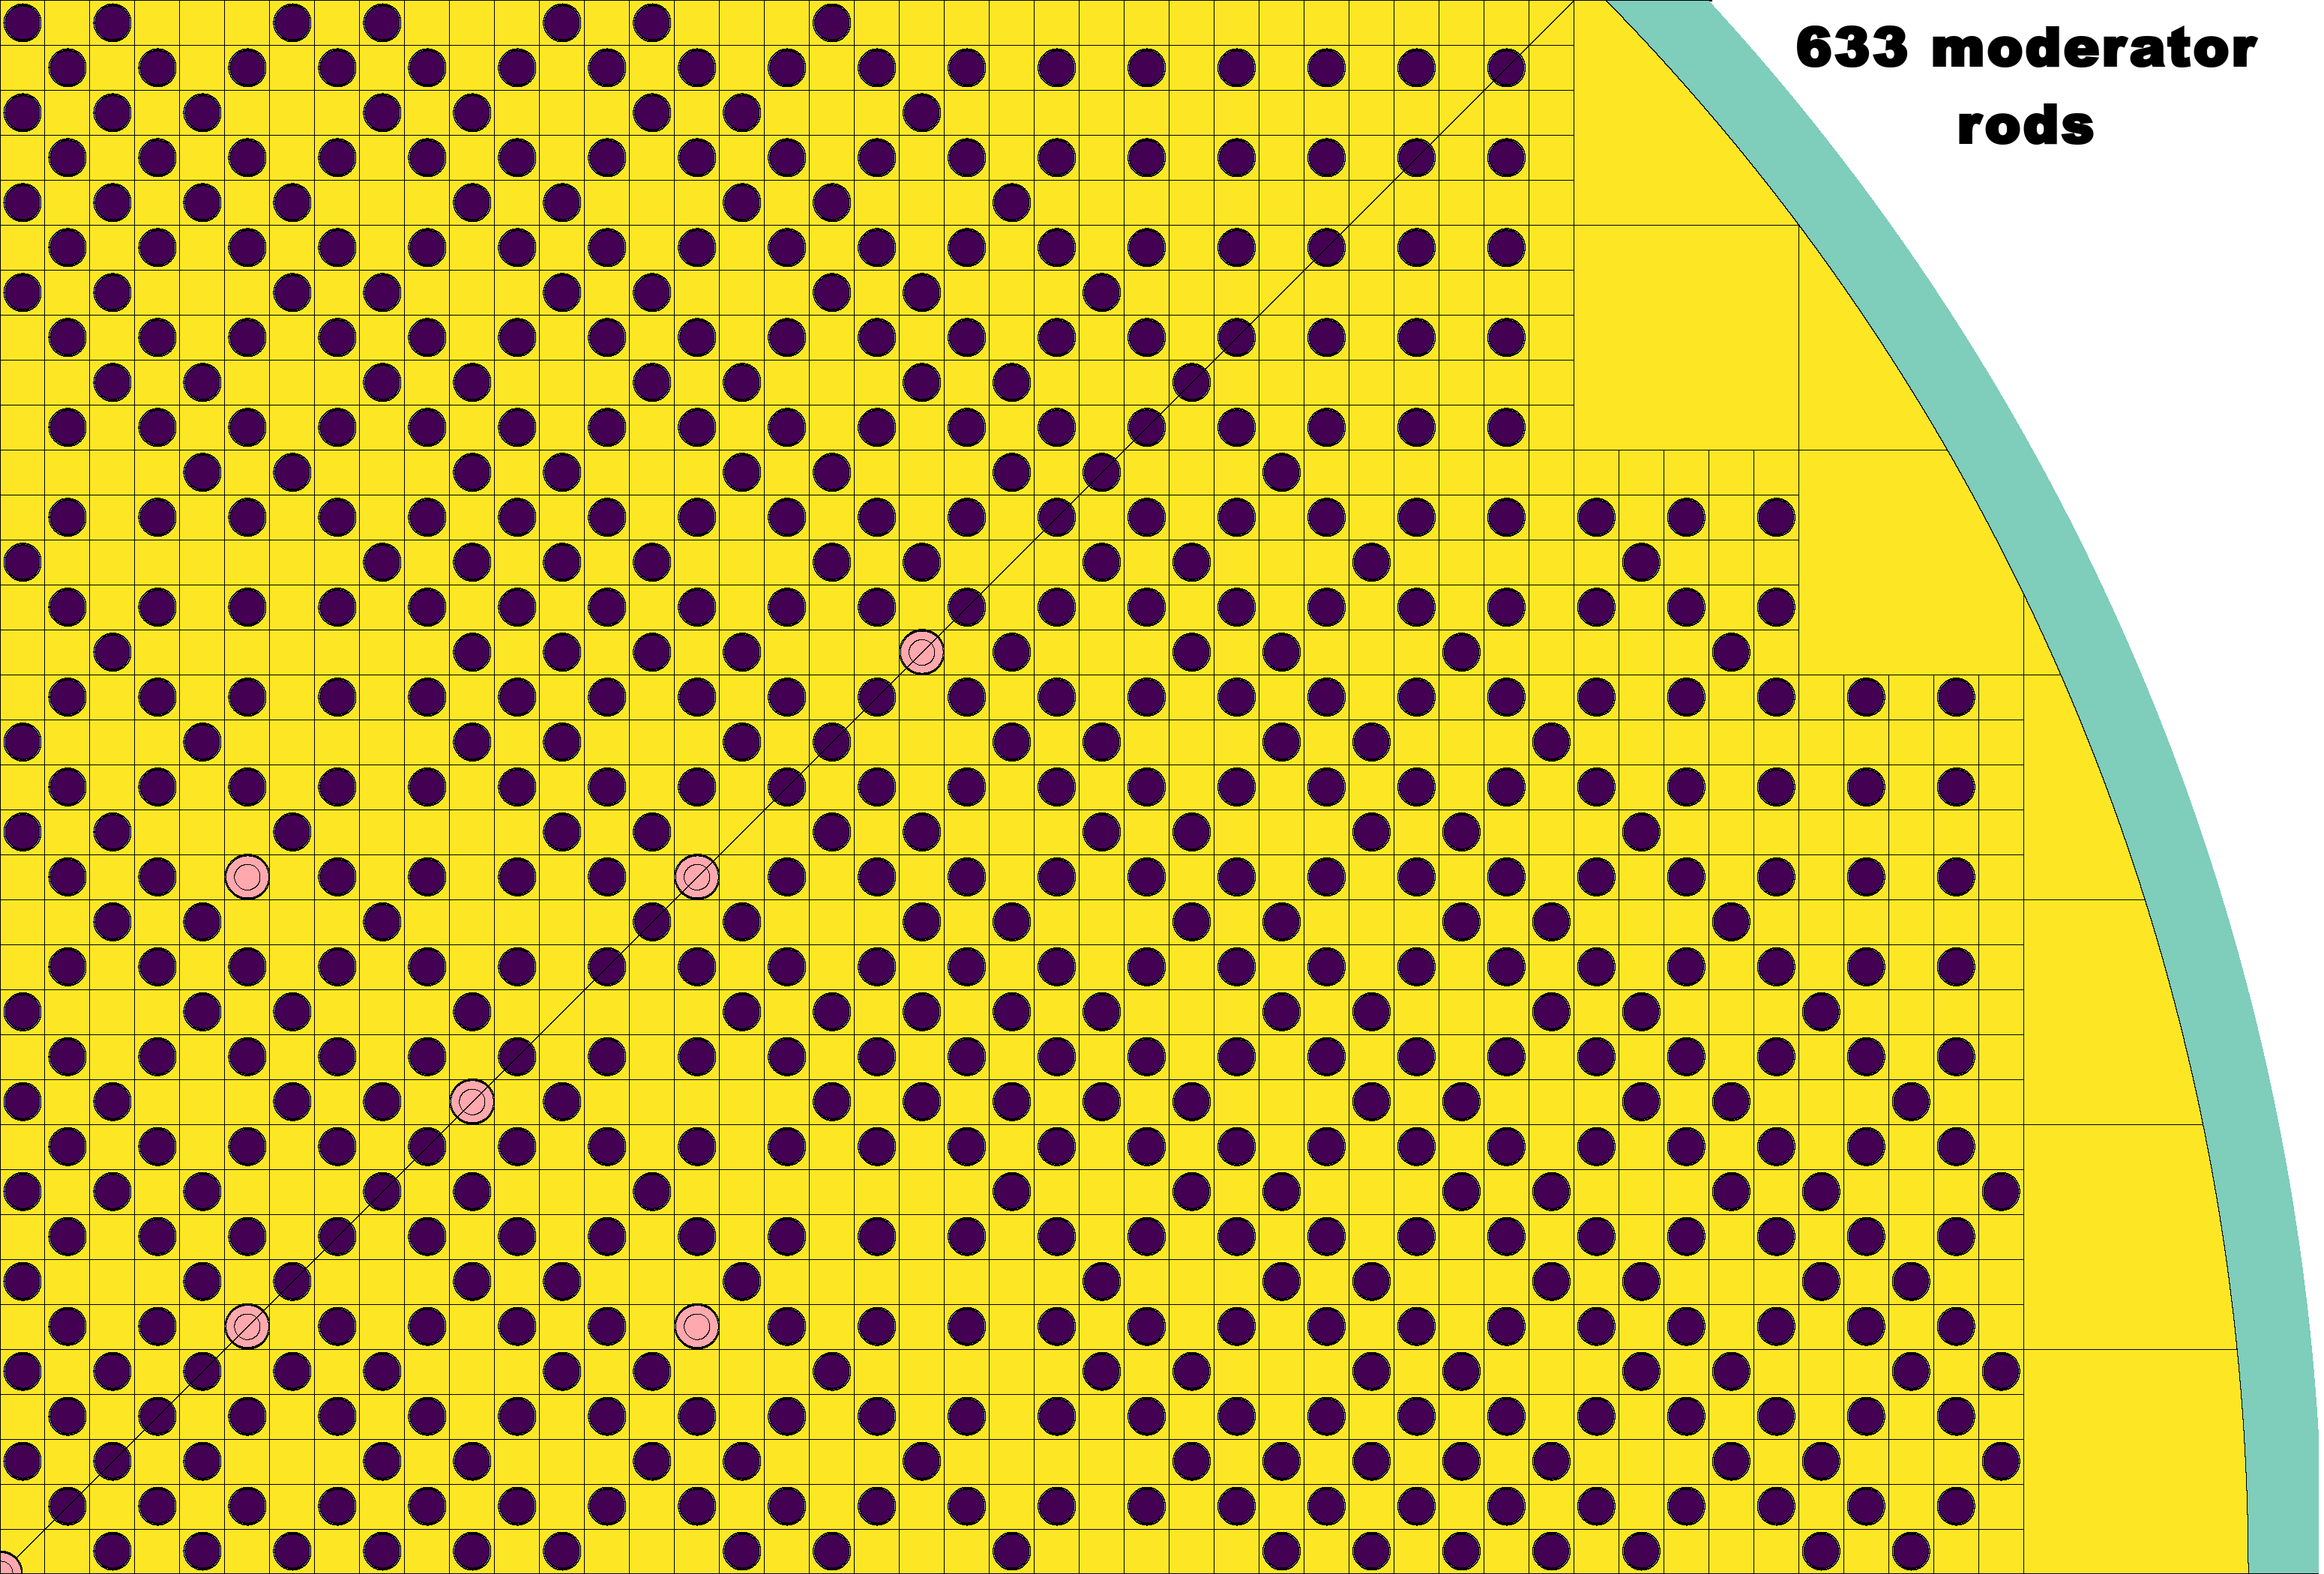
\includegraphics[height=0.75\textheight]{./images/633.png}}
		\onslide<5>\centerline{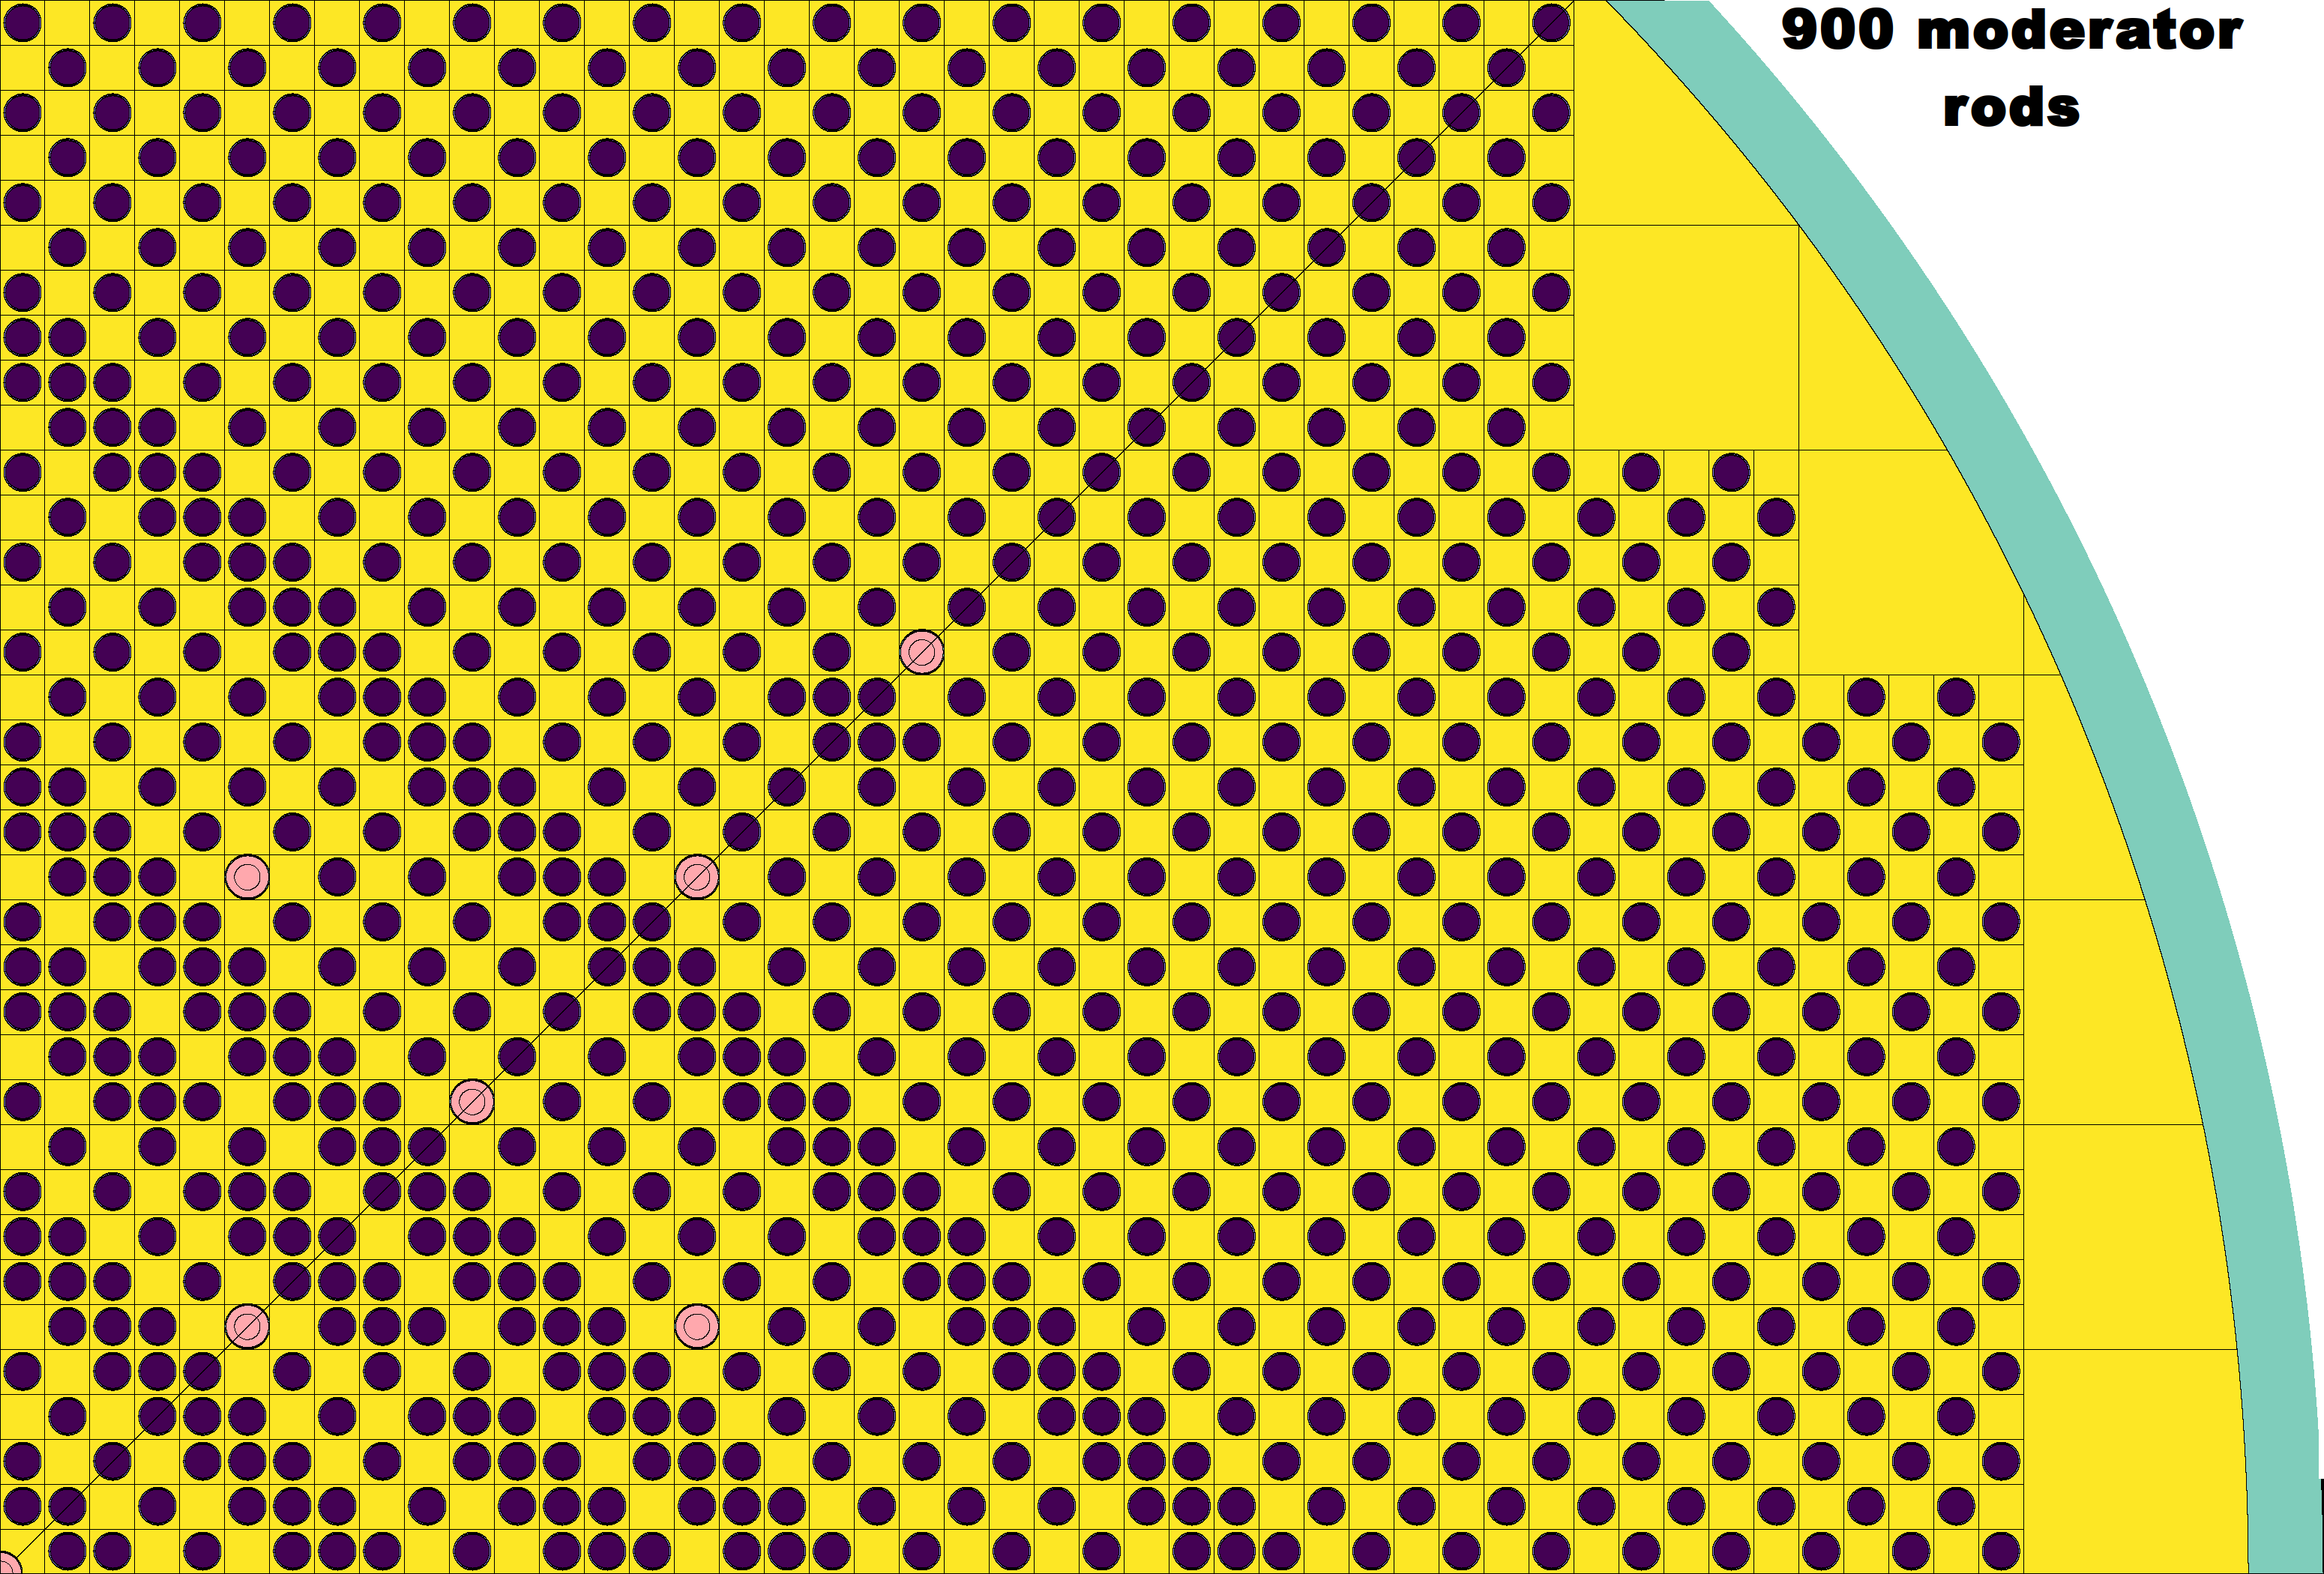
\includegraphics[height=0.75\textheight]{./images/900.png}}
		\onslide<6>\centerline{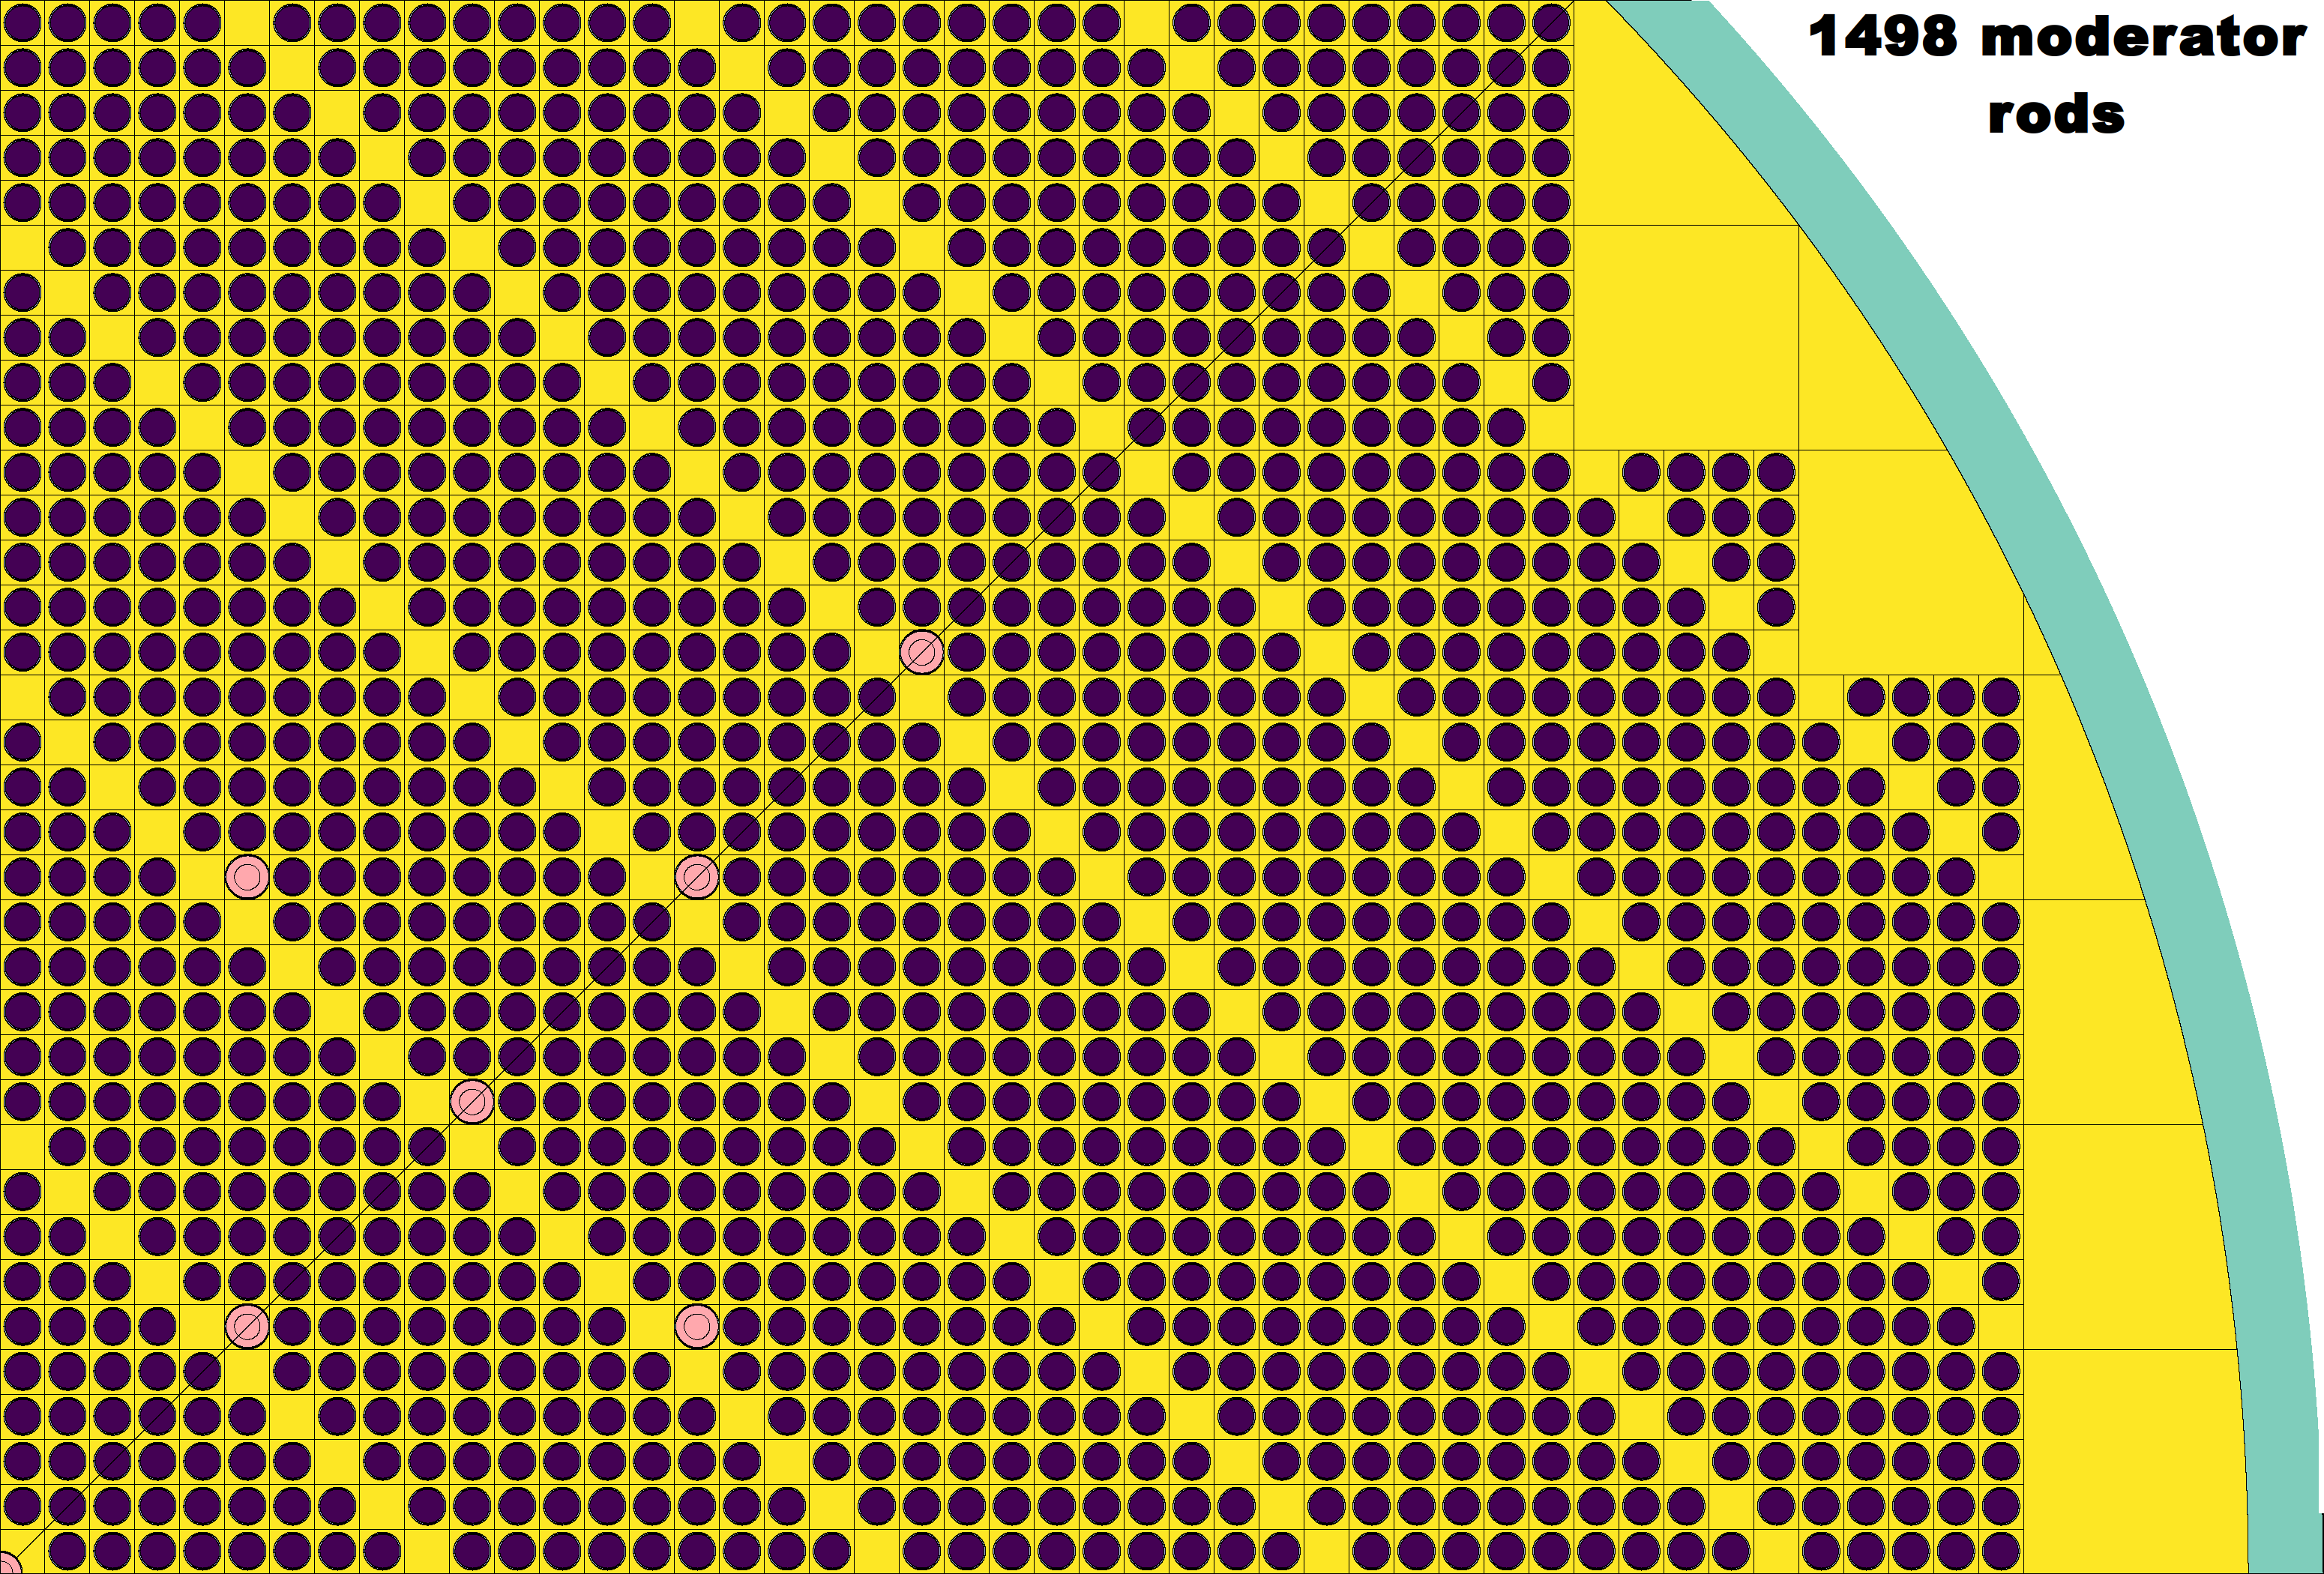
\includegraphics[height=0.75\textheight]{./images/1498.png}}
		\onslide<7>\centerline{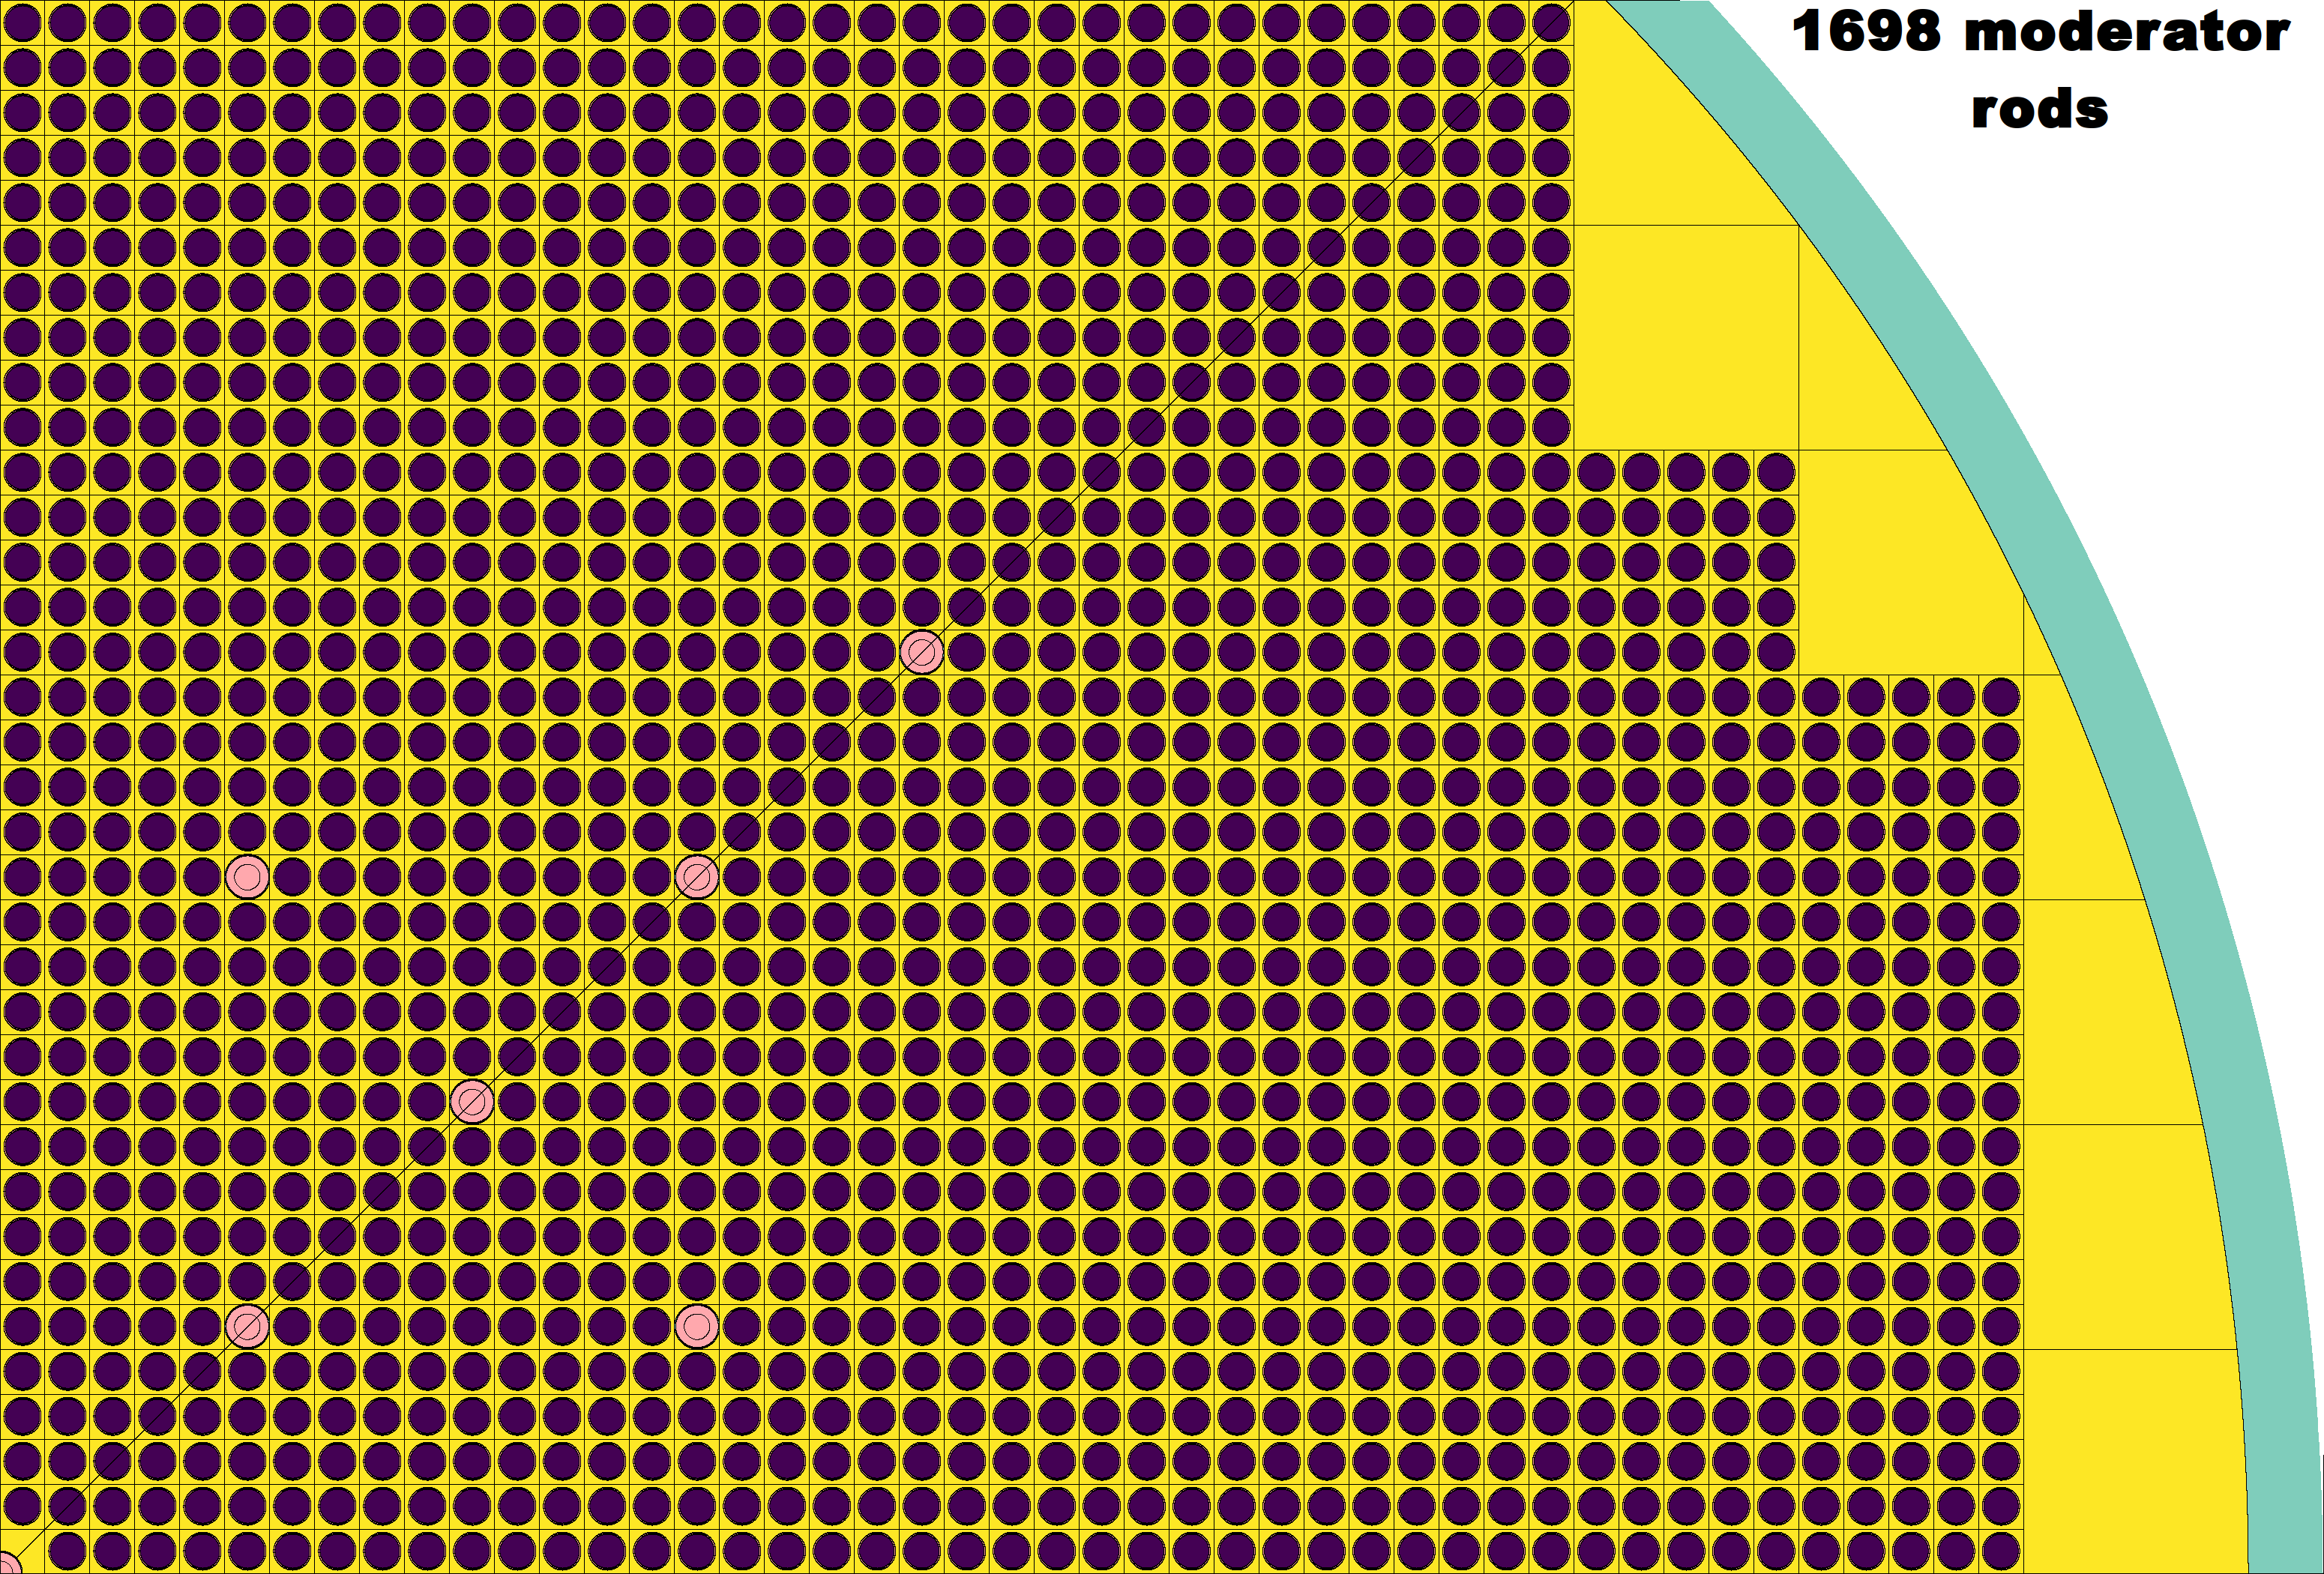
\includegraphics[height=0.75\textheight]{./images/1668.png}}
	\end{overprint}
	\caption{An $XY$ section of the \gls{TAP} model with various 
	moderator-to-fuel ratio. The violet color represents zirconium hydride, 
	the yellow represents fuel salt \cite{chaube_tap_2019, 
	rykhlevskii_milestone_2019}.}
\end{figure}
\end{textblock*}
\end{frame}



\begin{frame}
\frametitle{$k_{eff}$ dynamics during 23.5 years of TAP operation}
\vspace{-3mm}
\begin{columns}
	\column{4.3cm}
	\begin{block}{Analysis assumptions}
		\fontsize{7}{9}\selectfont
		\begin{itemize}
			\item Quarter-core Serpent model
			\item Fine depletion resolution (\textbf{3-day})
			\item 5\% LEU feed (UF$_4$) to maintain salt inventory
			\item Xe removal efficiency $\epsilon_{Xe}=$\textcolor{green}{
			0.03}, \textcolor{orange}{0.54}, and \textcolor{blue}{0.92} for 
			mass transfer coefficient $K_L=$\textcolor{green}{0.085}, 
			\textcolor{orange}{2.117}, and \textcolor{blue}{8.467}$mm/s$
		\end{itemize}
	\end{block}
	\vspace{-2mm}
	\begin{block}{Main findings}
		\fontsize{7}{9}\selectfont
		\begin{itemize}
			\item $^{235}$U is substituted with $^{239}$Pu
			\item Poisonous $^{234}$U is built-up ($>$1t at EOL)
			\item Total U inventory decreased from 137 to 129t
		\end{itemize}  
	\end{block}  	
	
	\column{8cm}
	\begin{figure}[ht!] 
		\begin{overprint}
			\onslide<1>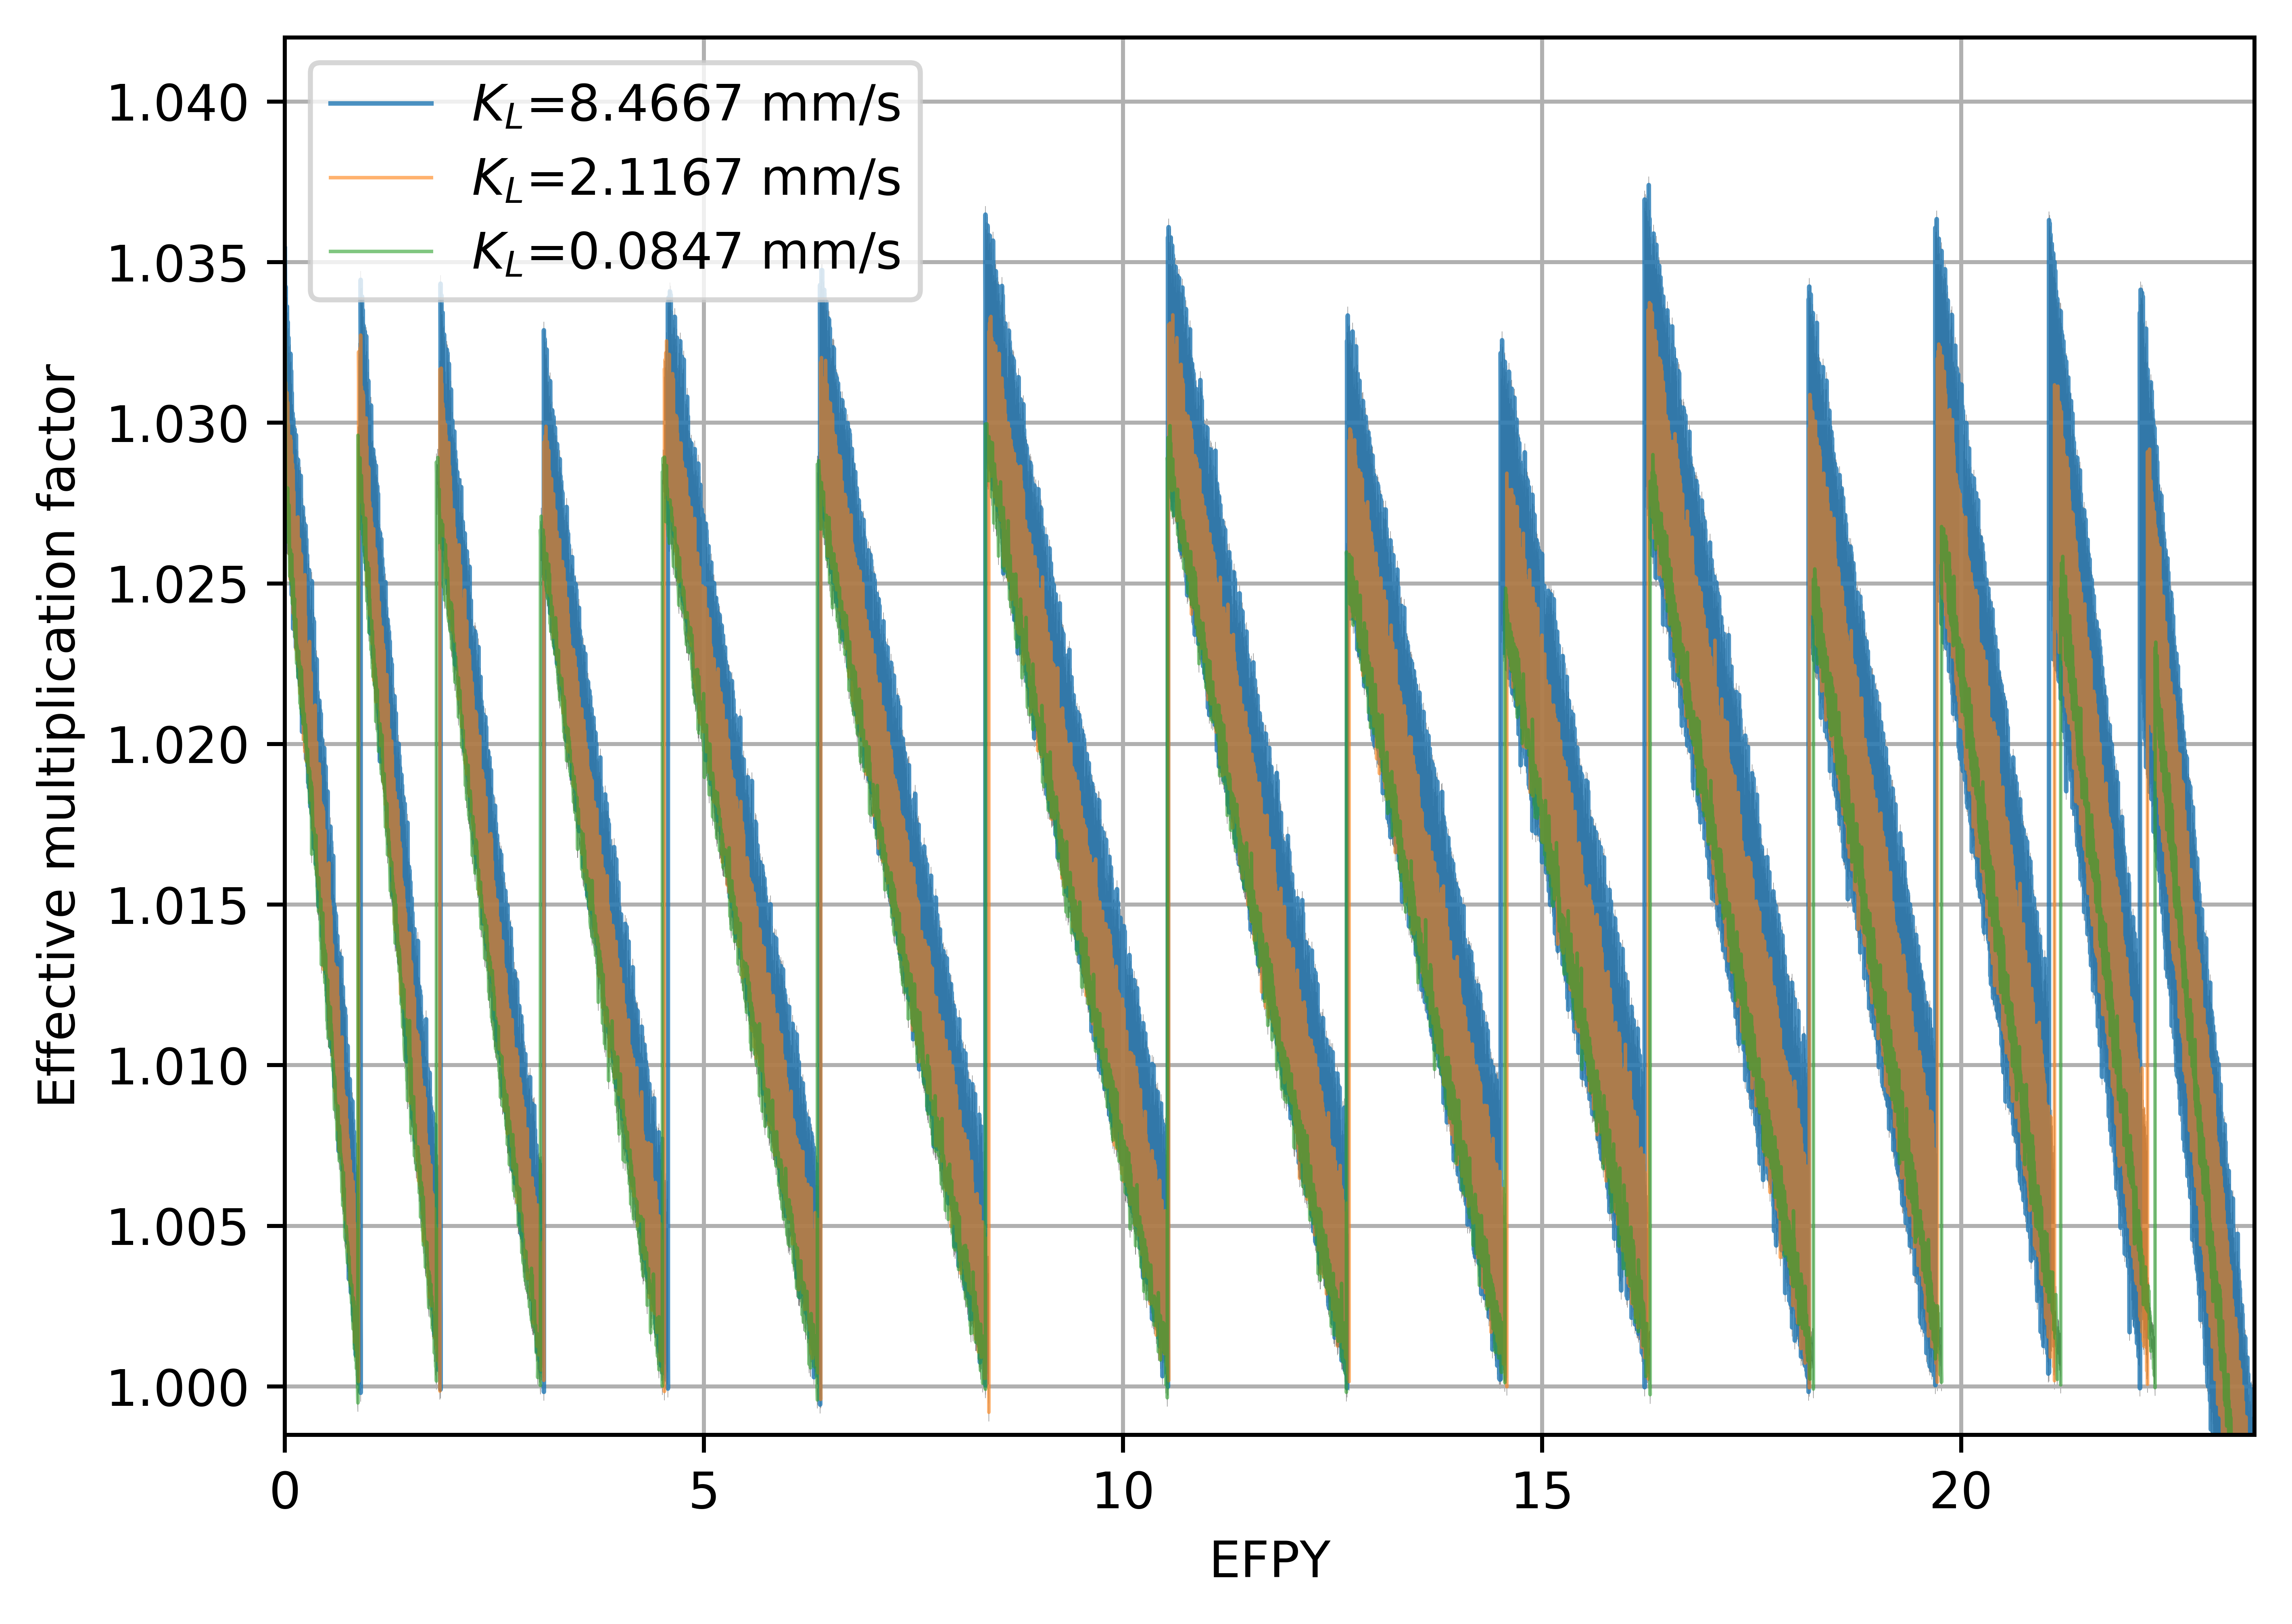
\includegraphics[width=\textwidth]{../dissertation/figures/ch4/eps/keff.png}
			\onslide<2>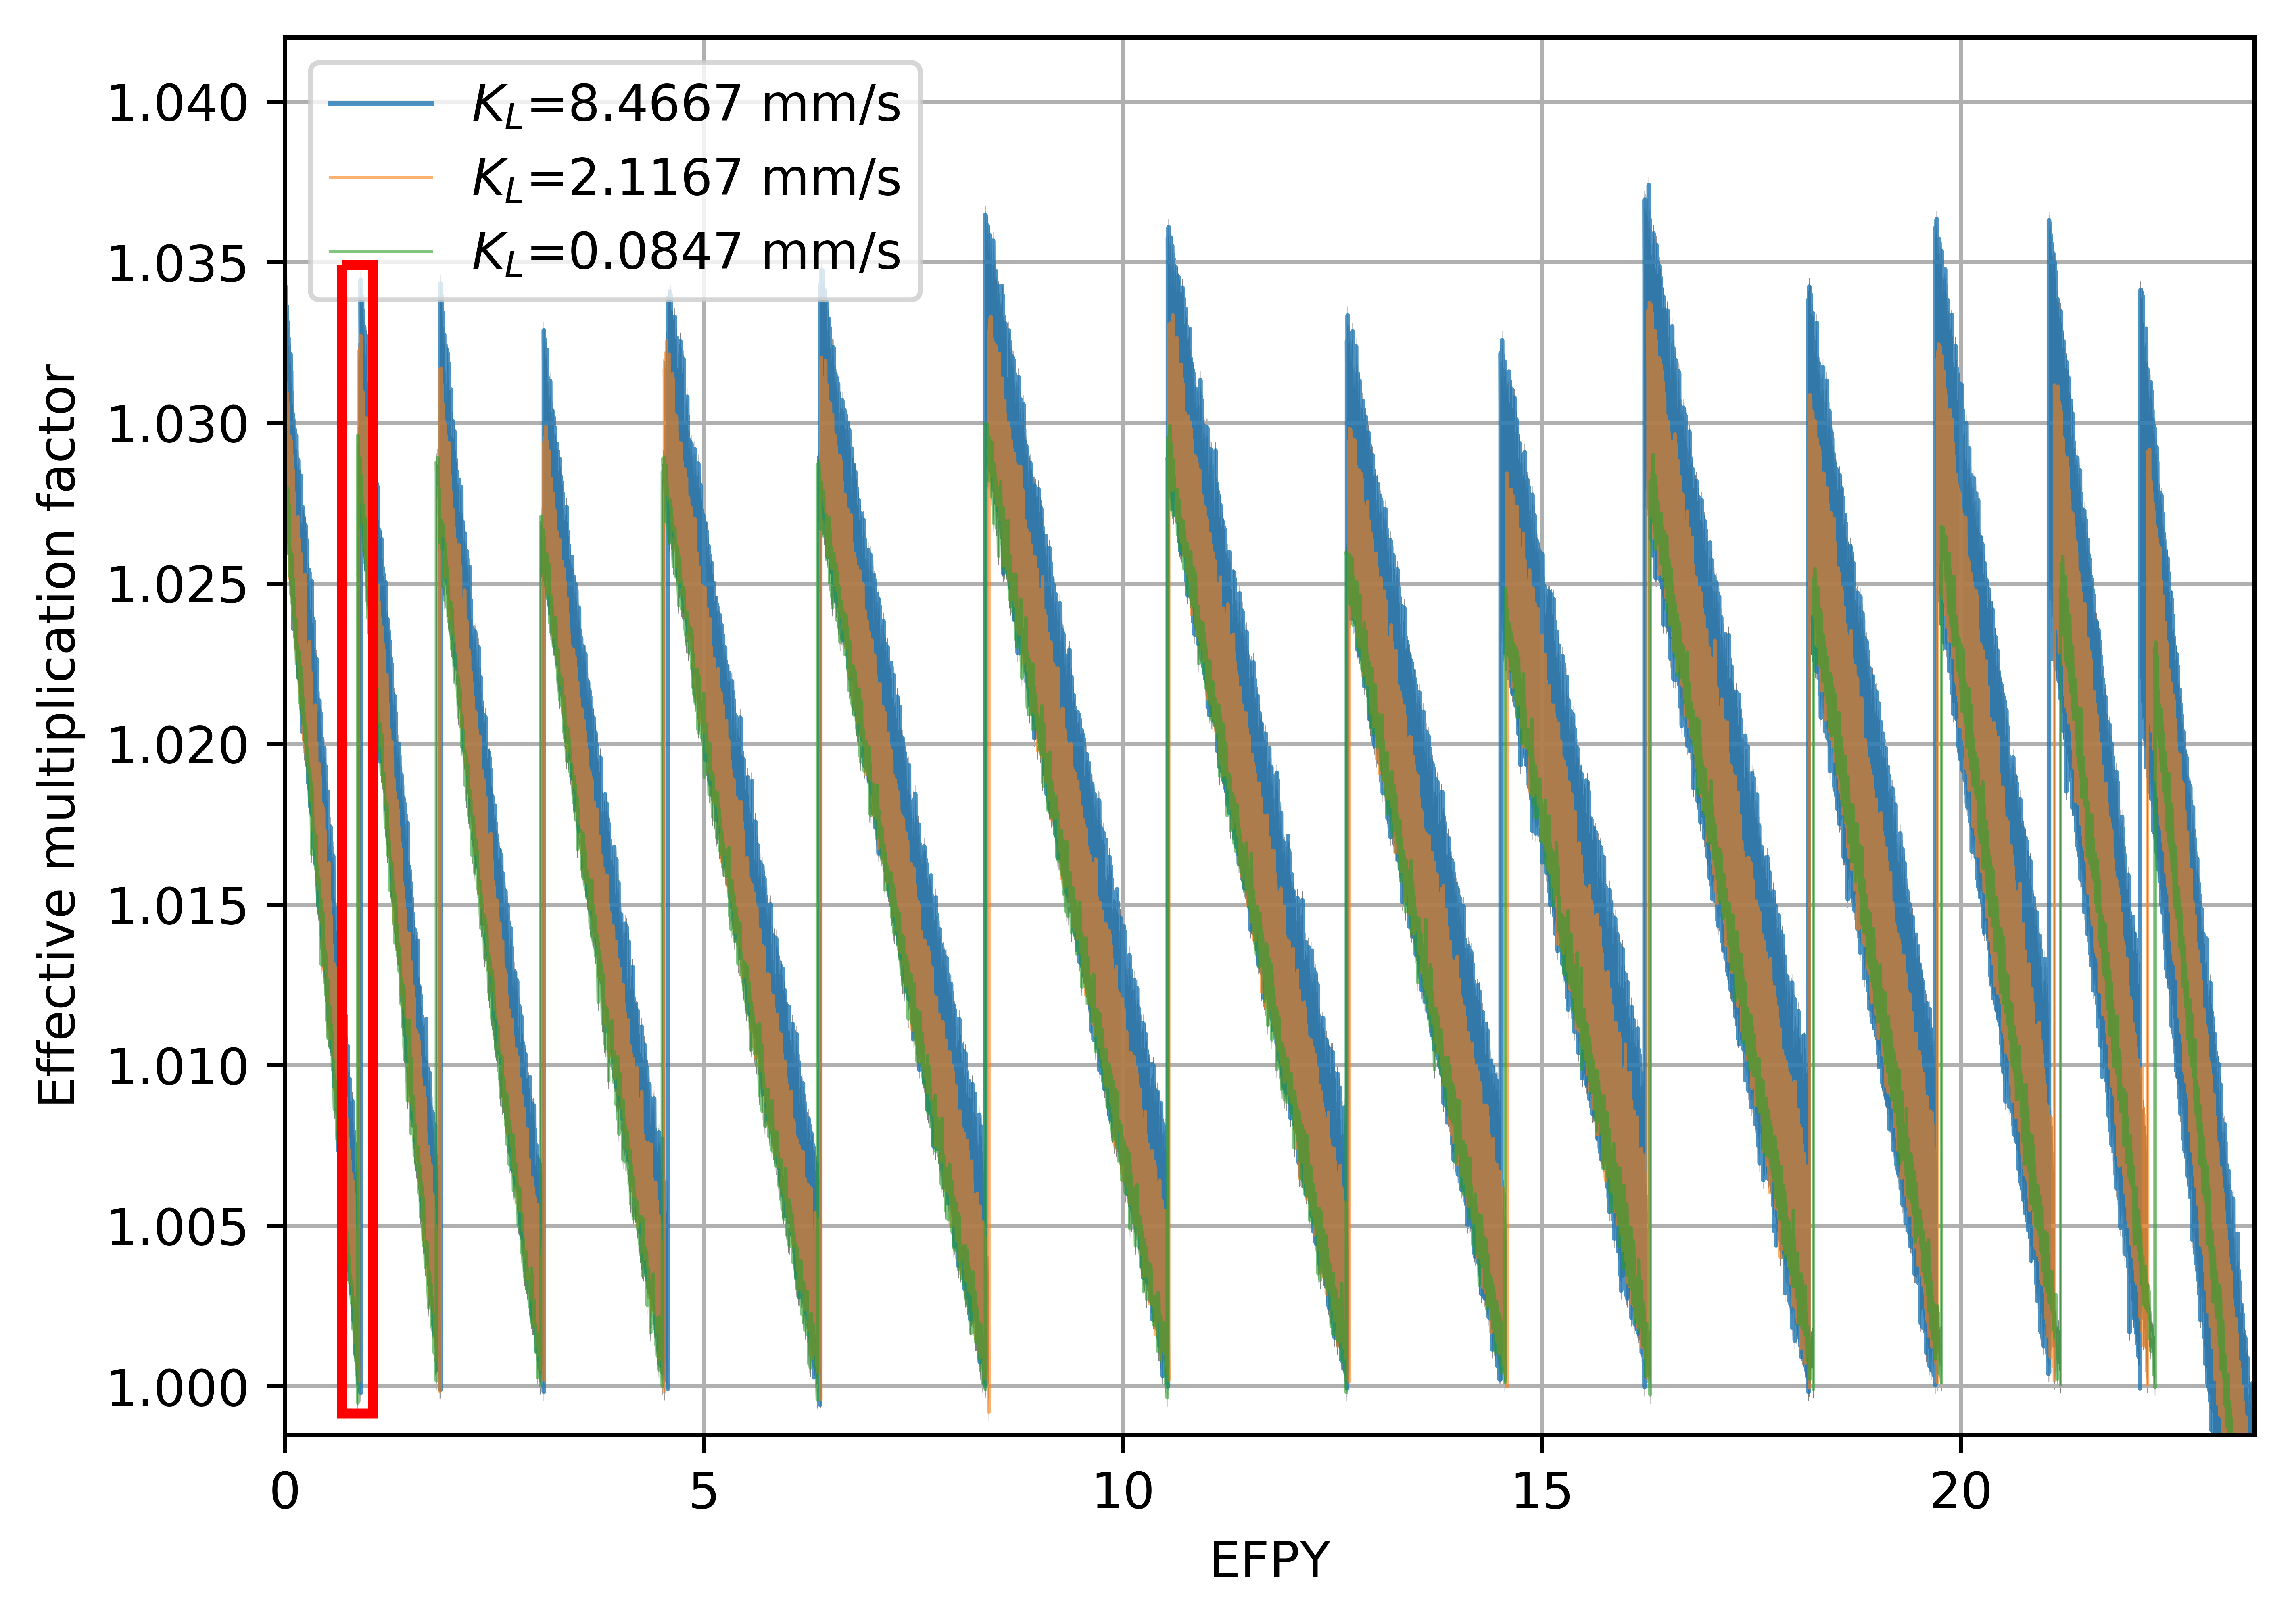
\includegraphics[width=\textwidth]{./images/keff_z_1.png}
			\onslide<3>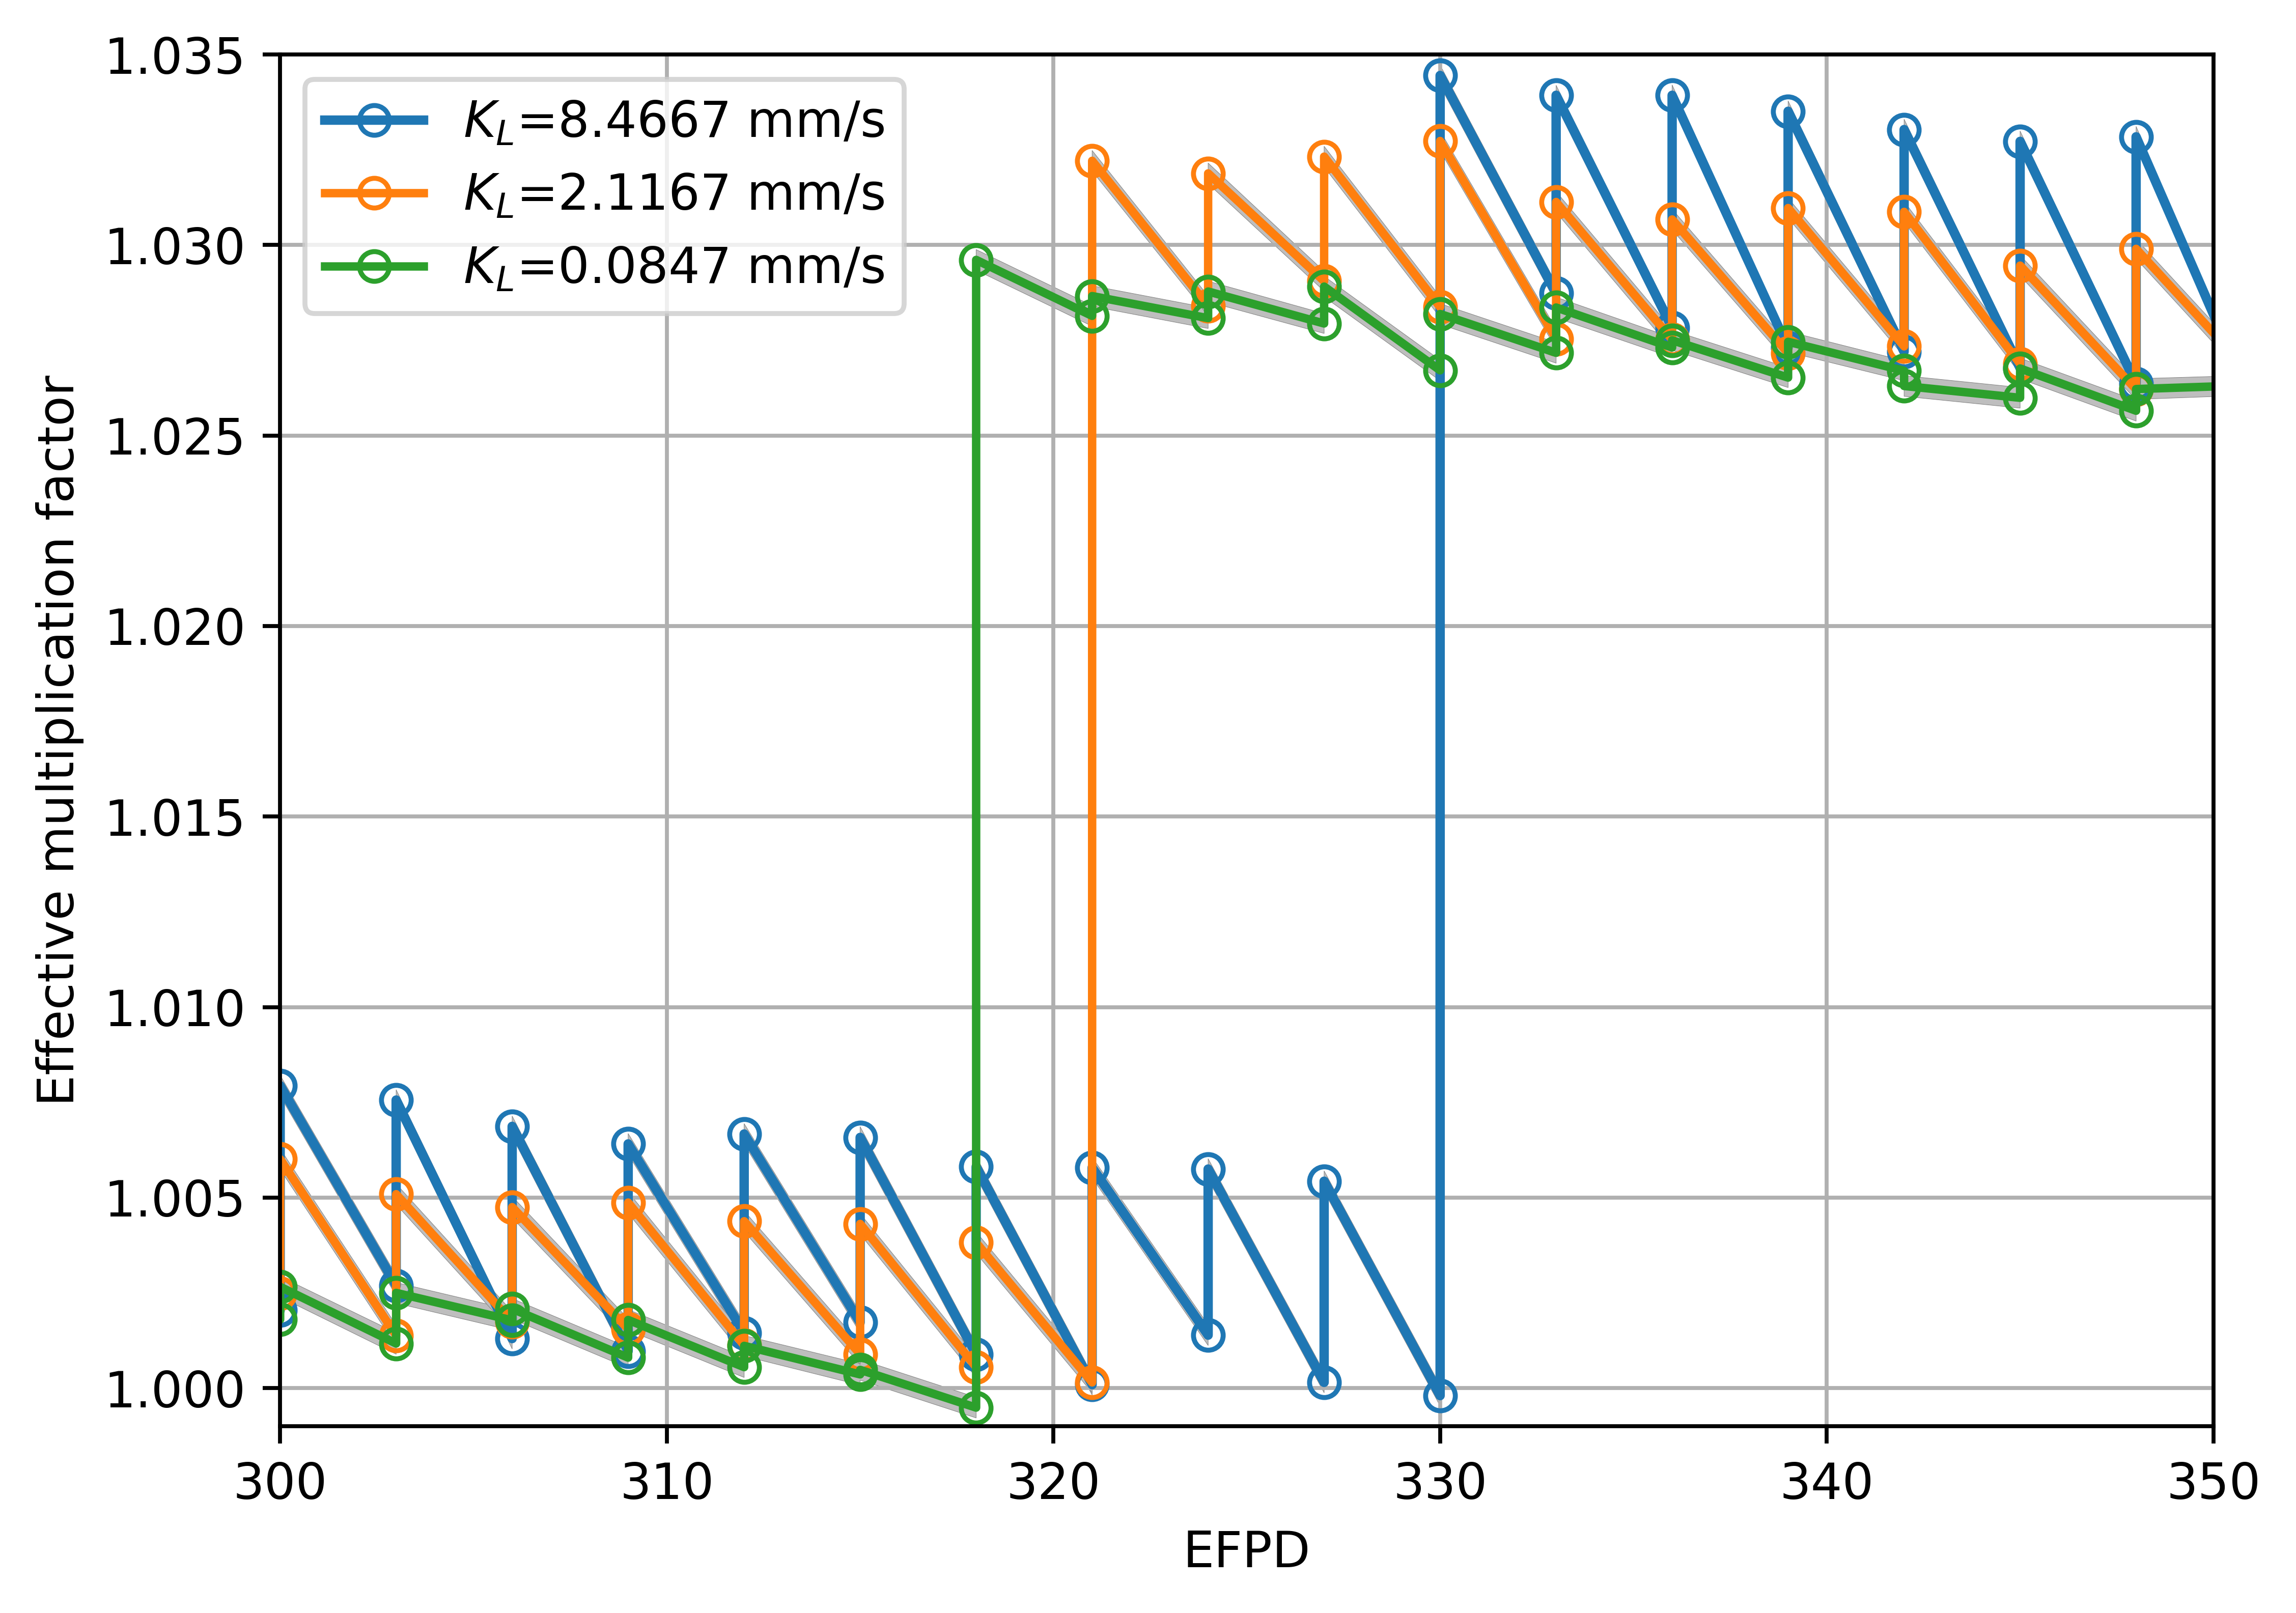
\includegraphics[width=\textwidth]{../dissertation/figures/ch4/eps/keff_zoomed_1.png}
			\vspace{-4mm}
		\end{overprint}
	\caption{SaltProc-calculated effective multiplication factor 
	for the full-core \gls{TAP} concept.}			
	\end{figure}
	
\end{columns}
\end{frame}


\begin{frame}
\frametitle{Neutron energy spectrum}
\begin{textblock*}{12.6cm}(0.1cm,1.7cm) % {block width} (coords)
	\begin{figure}[htp!] % replace 't' with 'b' to 
		\begin{overprint}
\onslide<1>\centerline{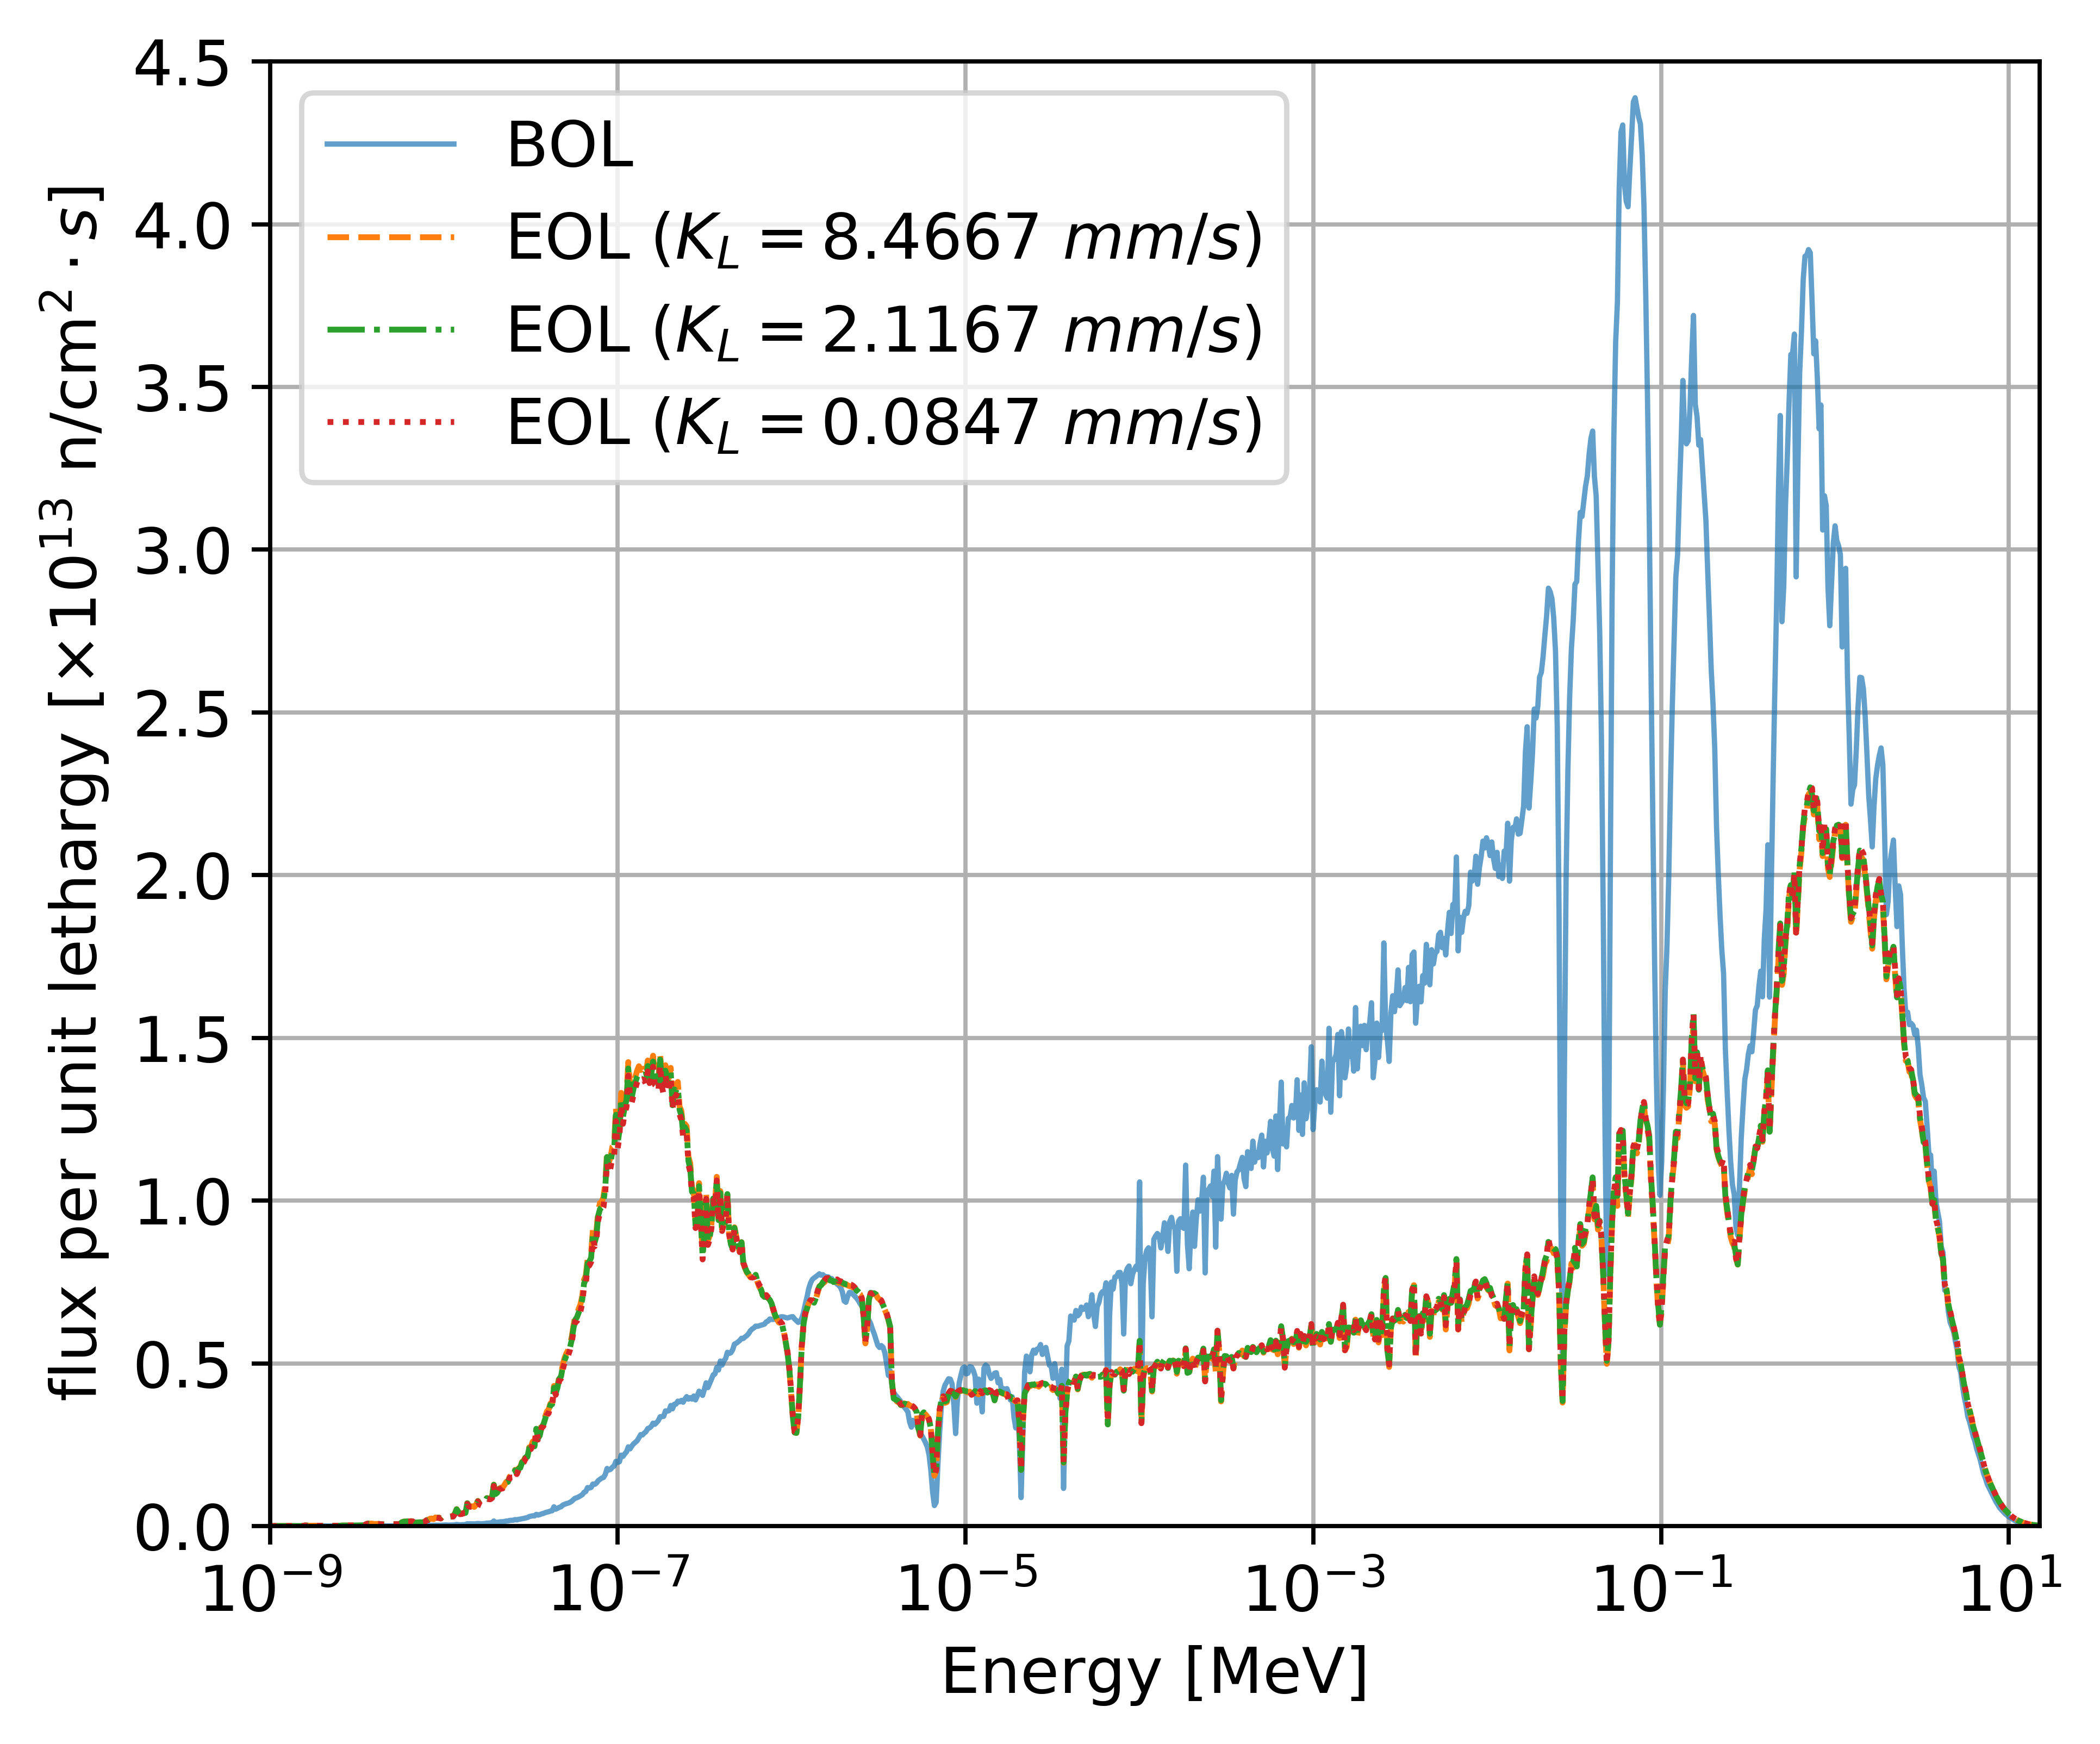
\includegraphics[width=0.65\textwidth]{../dissertation/figures/ch4/eps/spectrum.png}}
\onslide<2>\centerline{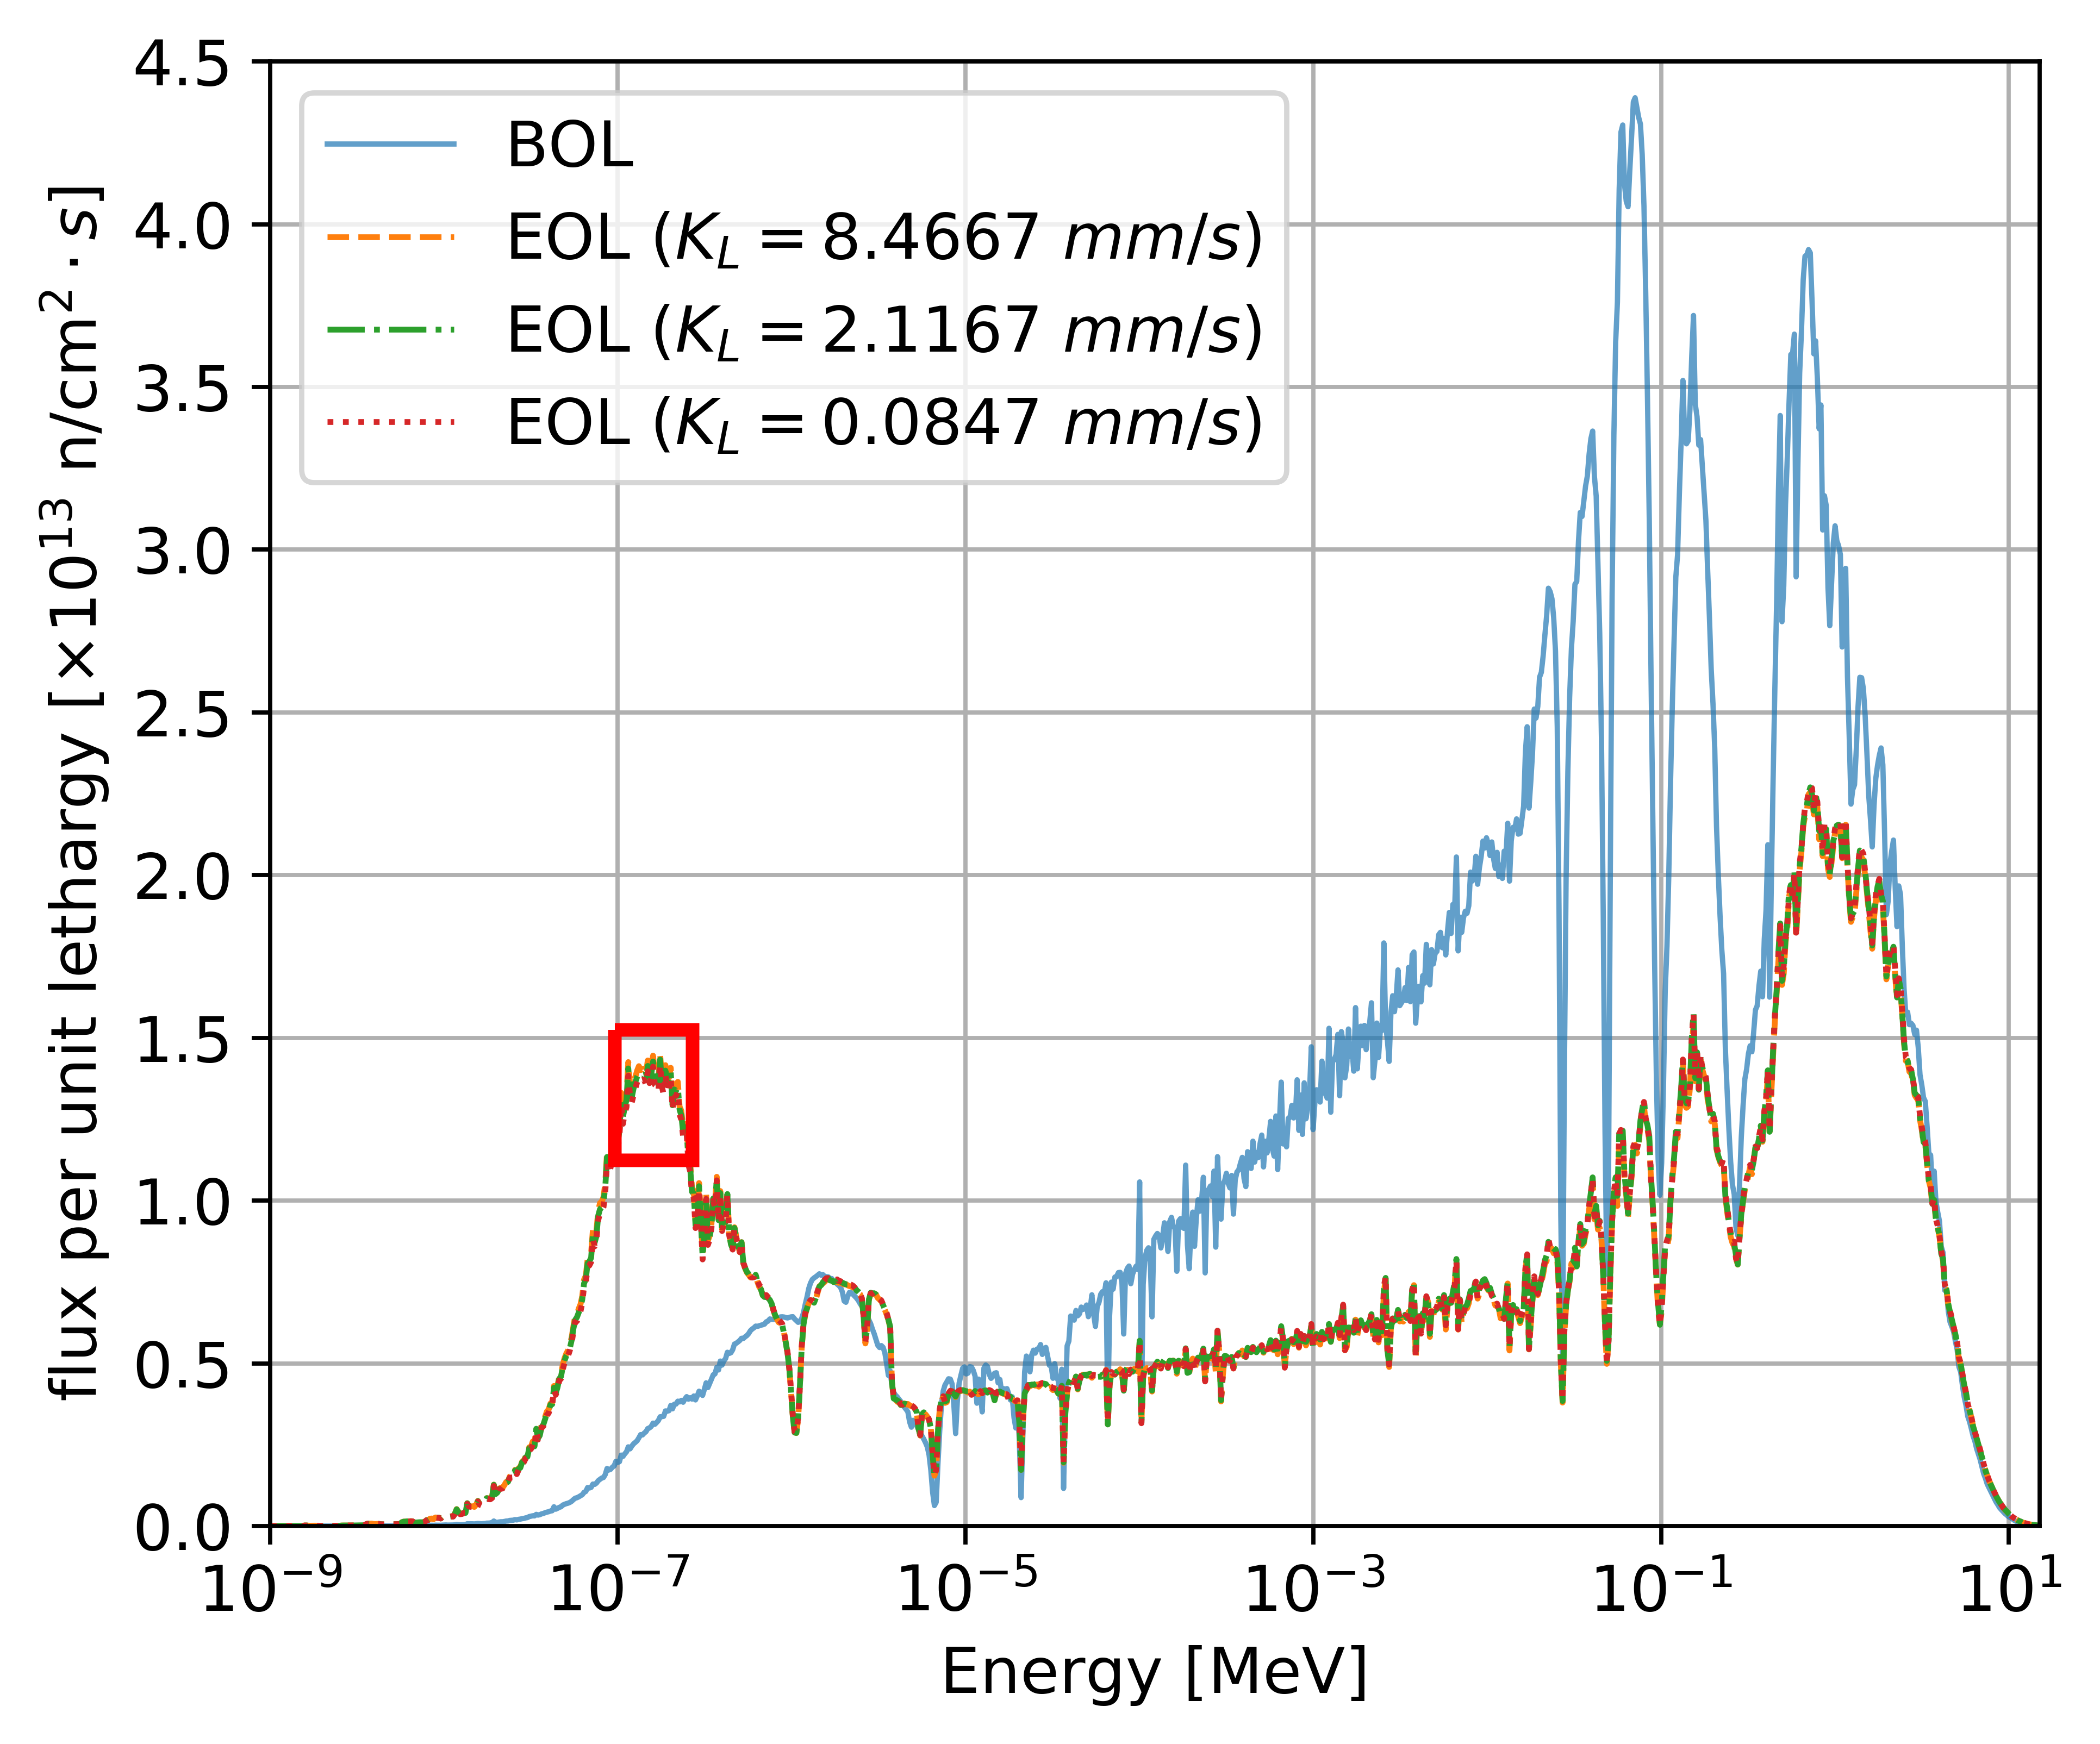
\includegraphics[width=0.65\textwidth]{./images/tap_sp_z_1.png}}
\onslide<3>\centerline{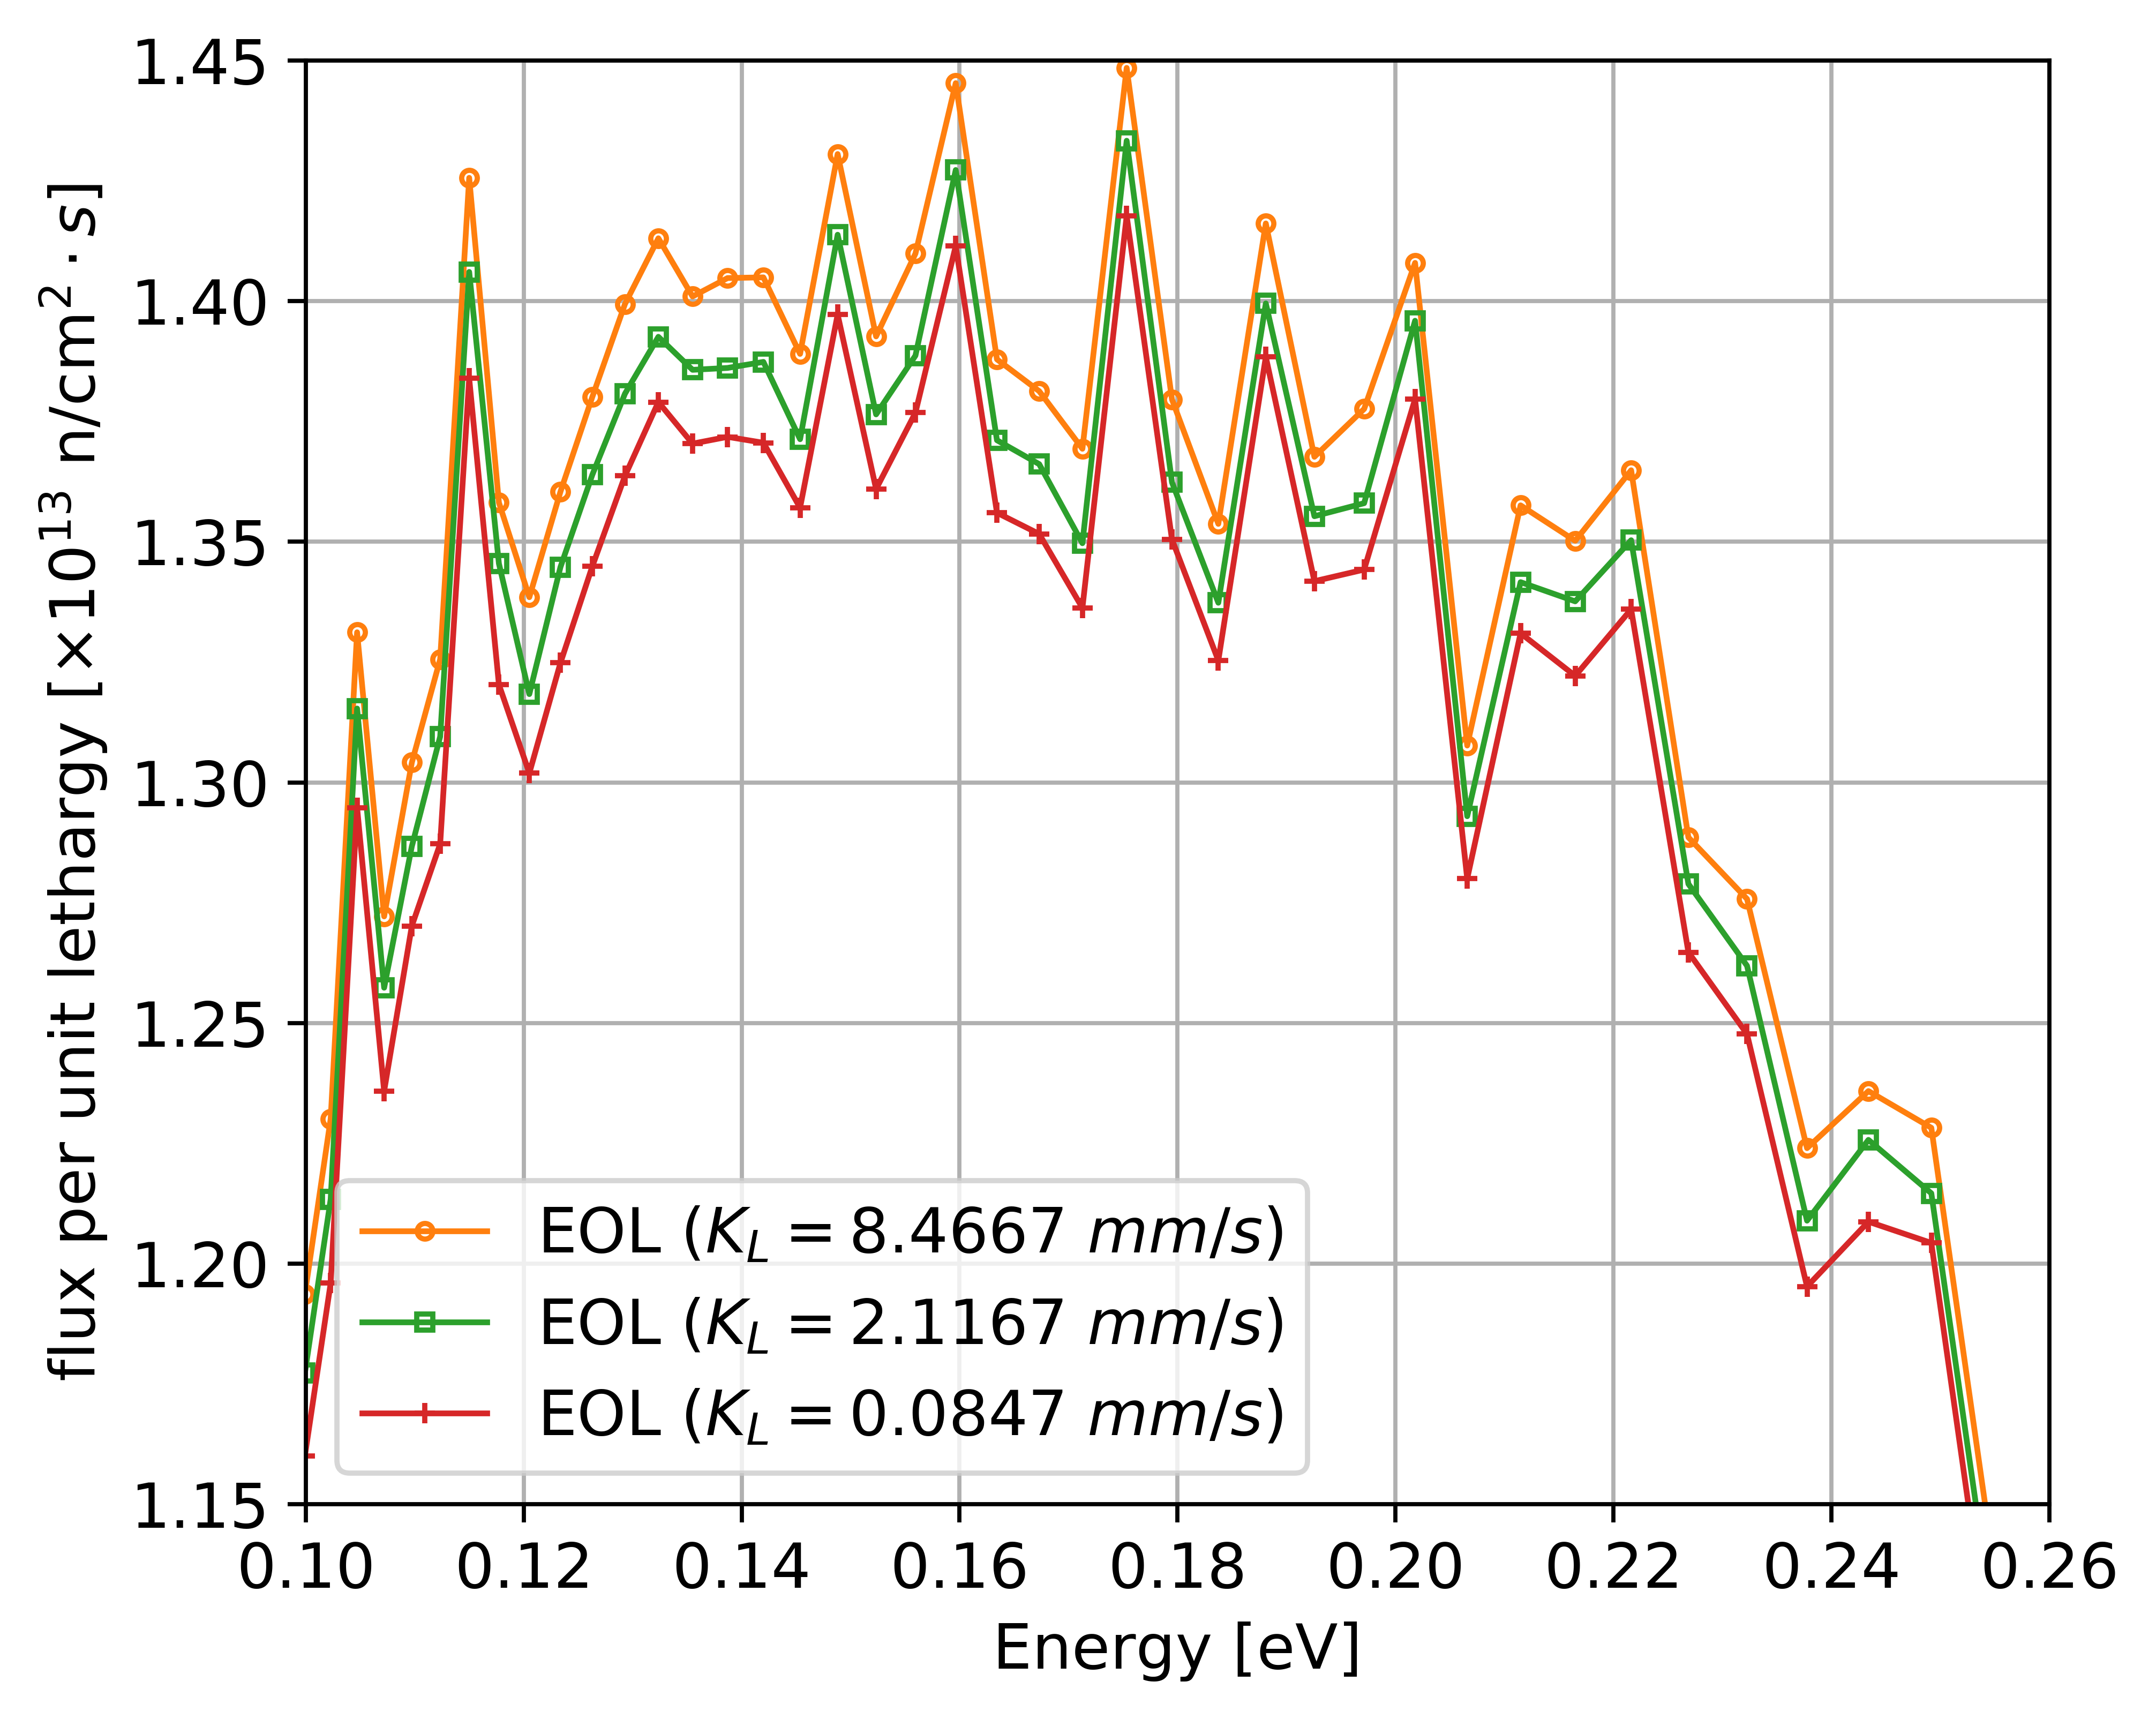
\includegraphics[width=0.67\textwidth]{../dissertation/figures/ch4/eps/spectrum_th_zoomed.png}}
		\end{overprint}
			\vspace{-3mm}
		\caption{The neutron flux energy spectrum normalized by unit lethargy 
		at the BOL and EOL. The neutron flux uncertainties $\sigma_{\Phi}$ are 
		0.6\% and 0.18\% for the \gls{TAP} reactor and \gls{MSBR}, 
		respectively.}
	\end{figure}
\end{textblock*}
\end{frame}


\begin{frame}
\frametitle{Fuel salt composition evolution during the TAP operation (1/2)}
\begin{textblock*}{12.25cm}(0.25cm,1.8cm) % {block width} (coords)
	\begin{figure}[htp!] % replace 't' with 'b' to 
		\centering
		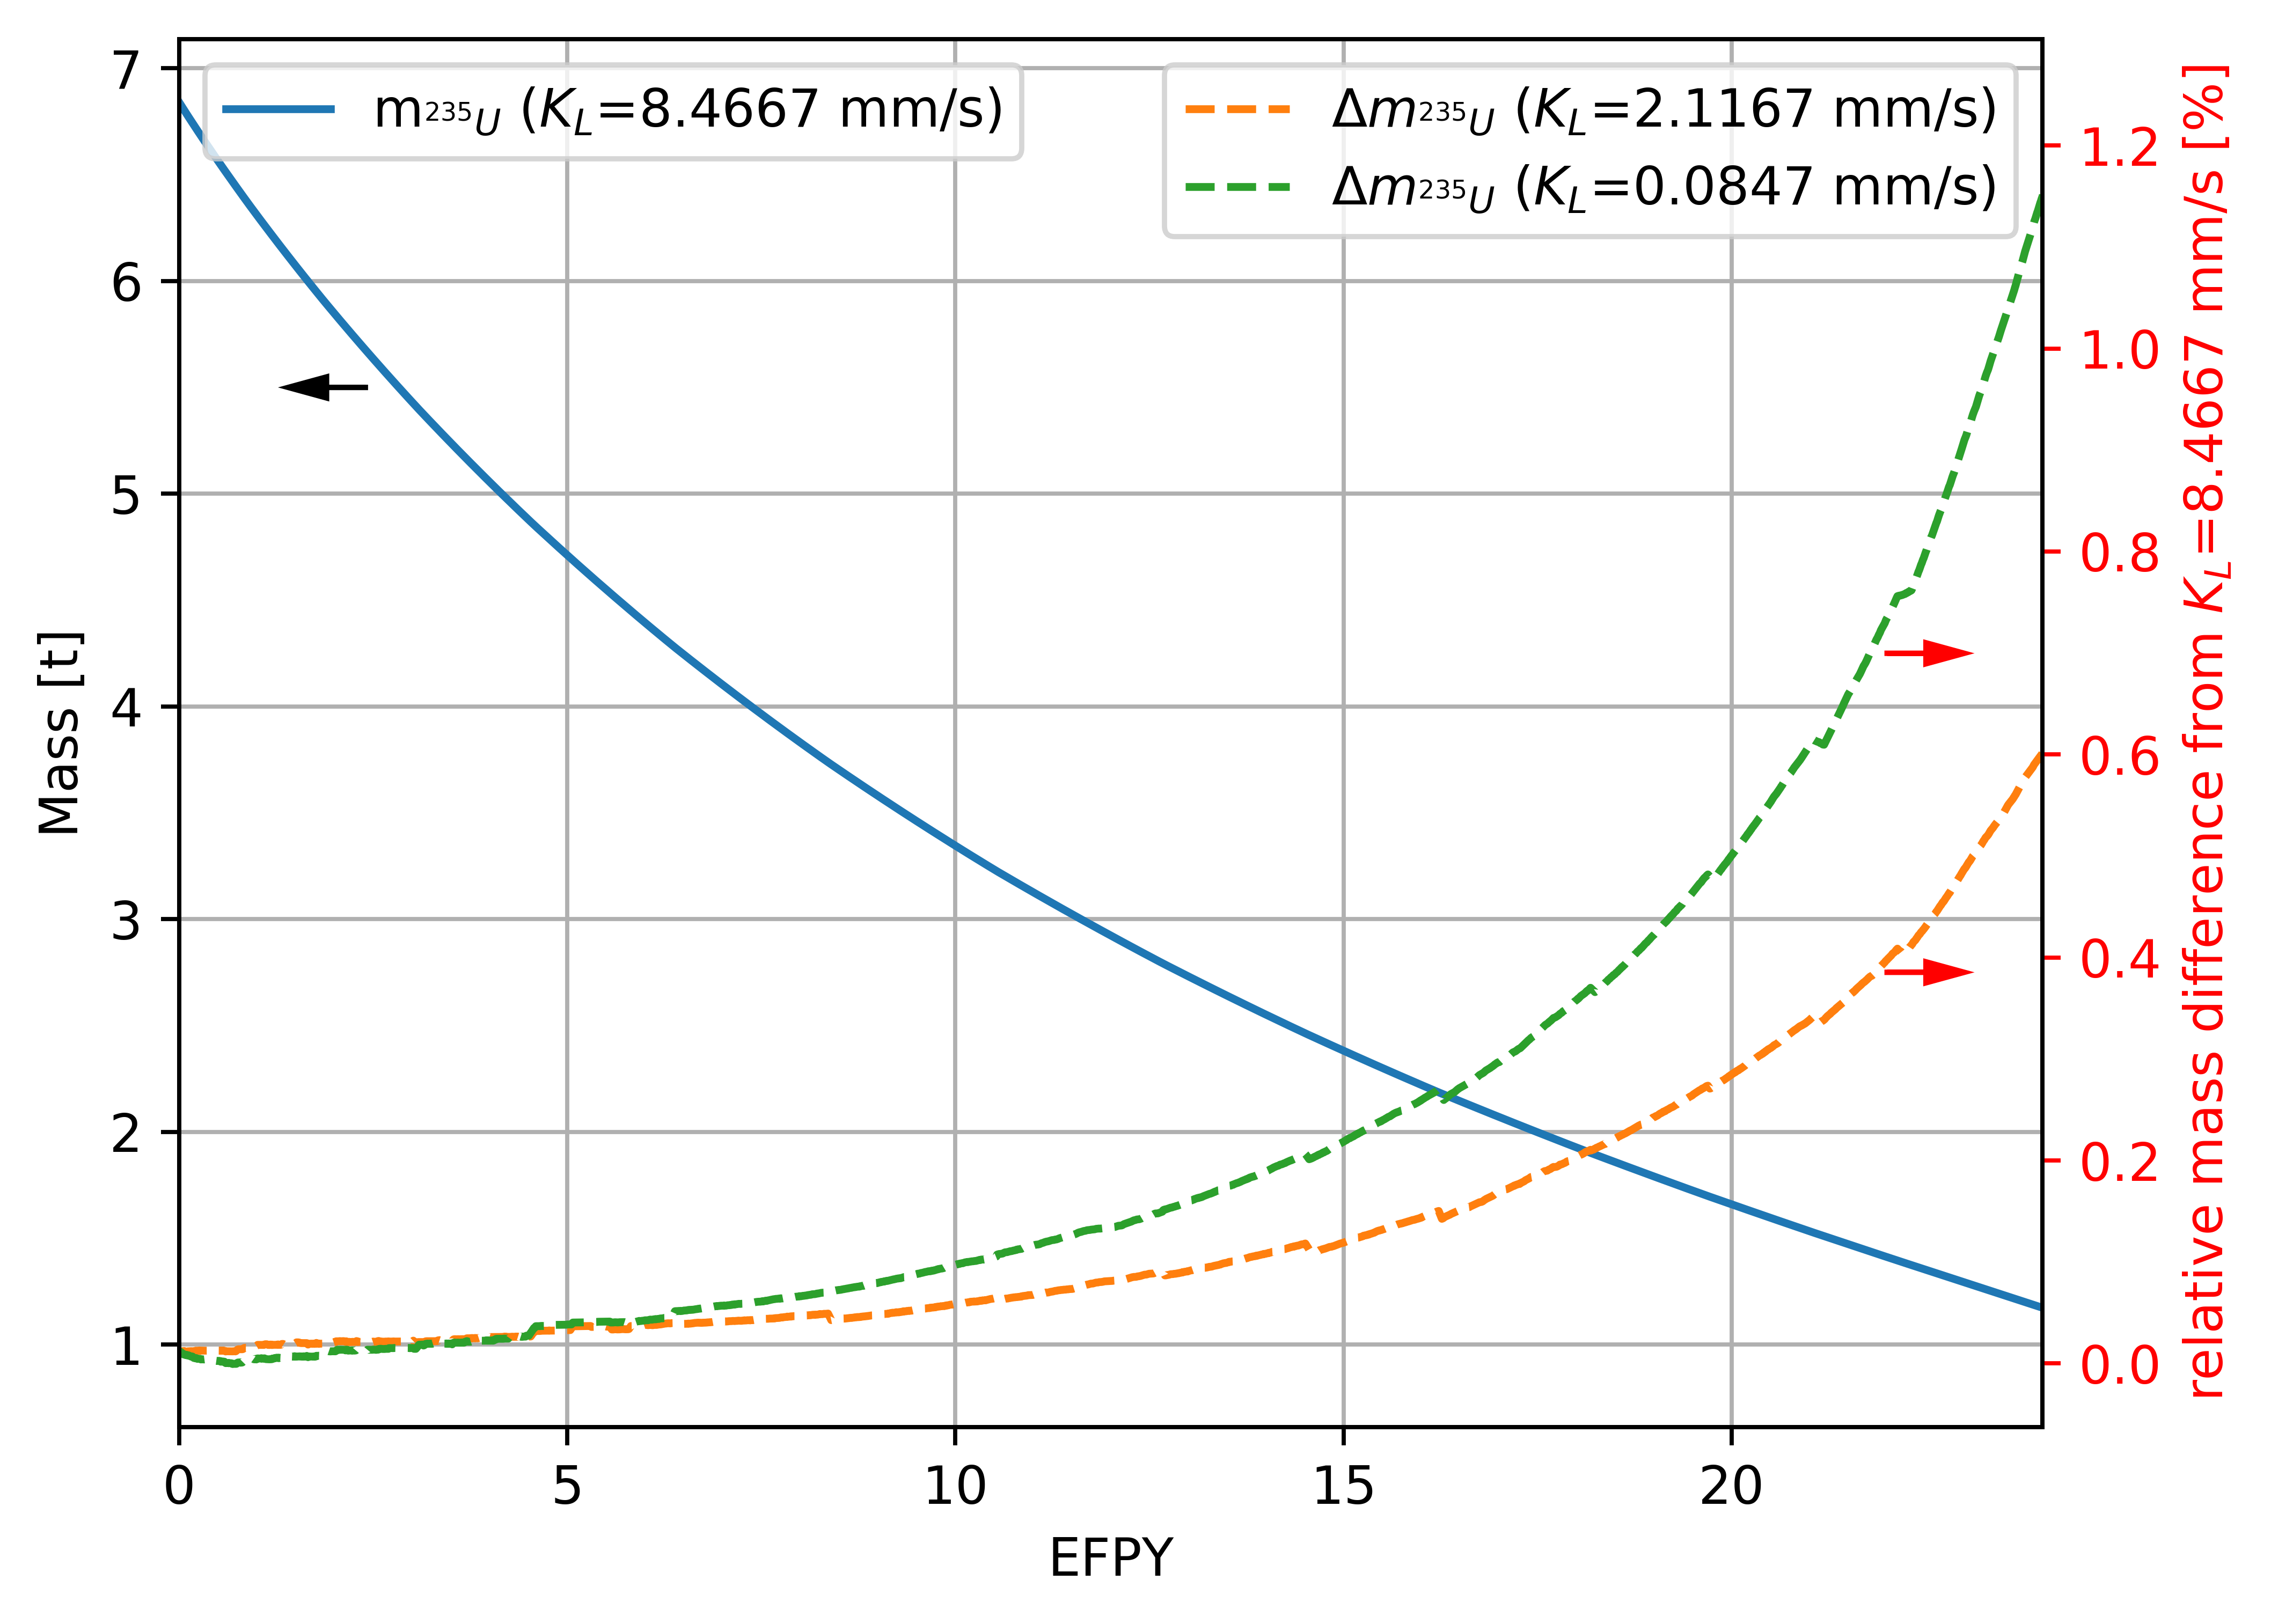
\includegraphics[width=0.75\textwidth]{../dissertation/figures/ch4/eps/u235.png}
			\vspace{-2mm}
		\caption{SaltProc-calculated mass of $^{235}$U in the fuel salt during 
		25 years of operation
for K$_L$ = 8.4667 mm/s compared with less 
		effective noble gas removal.}
	\end{figure}
\end{textblock*}
\end{frame}

\begin{frame}
\frametitle{Fuel salt composition evolution during the TAP operation (2/2)}
\begin{textblock*}{12.25cm}(0.25cm,1.8cm) % {block width} (coords)
	\begin{figure}[htp!] % replace 't' with 'b' to 
		\centering
		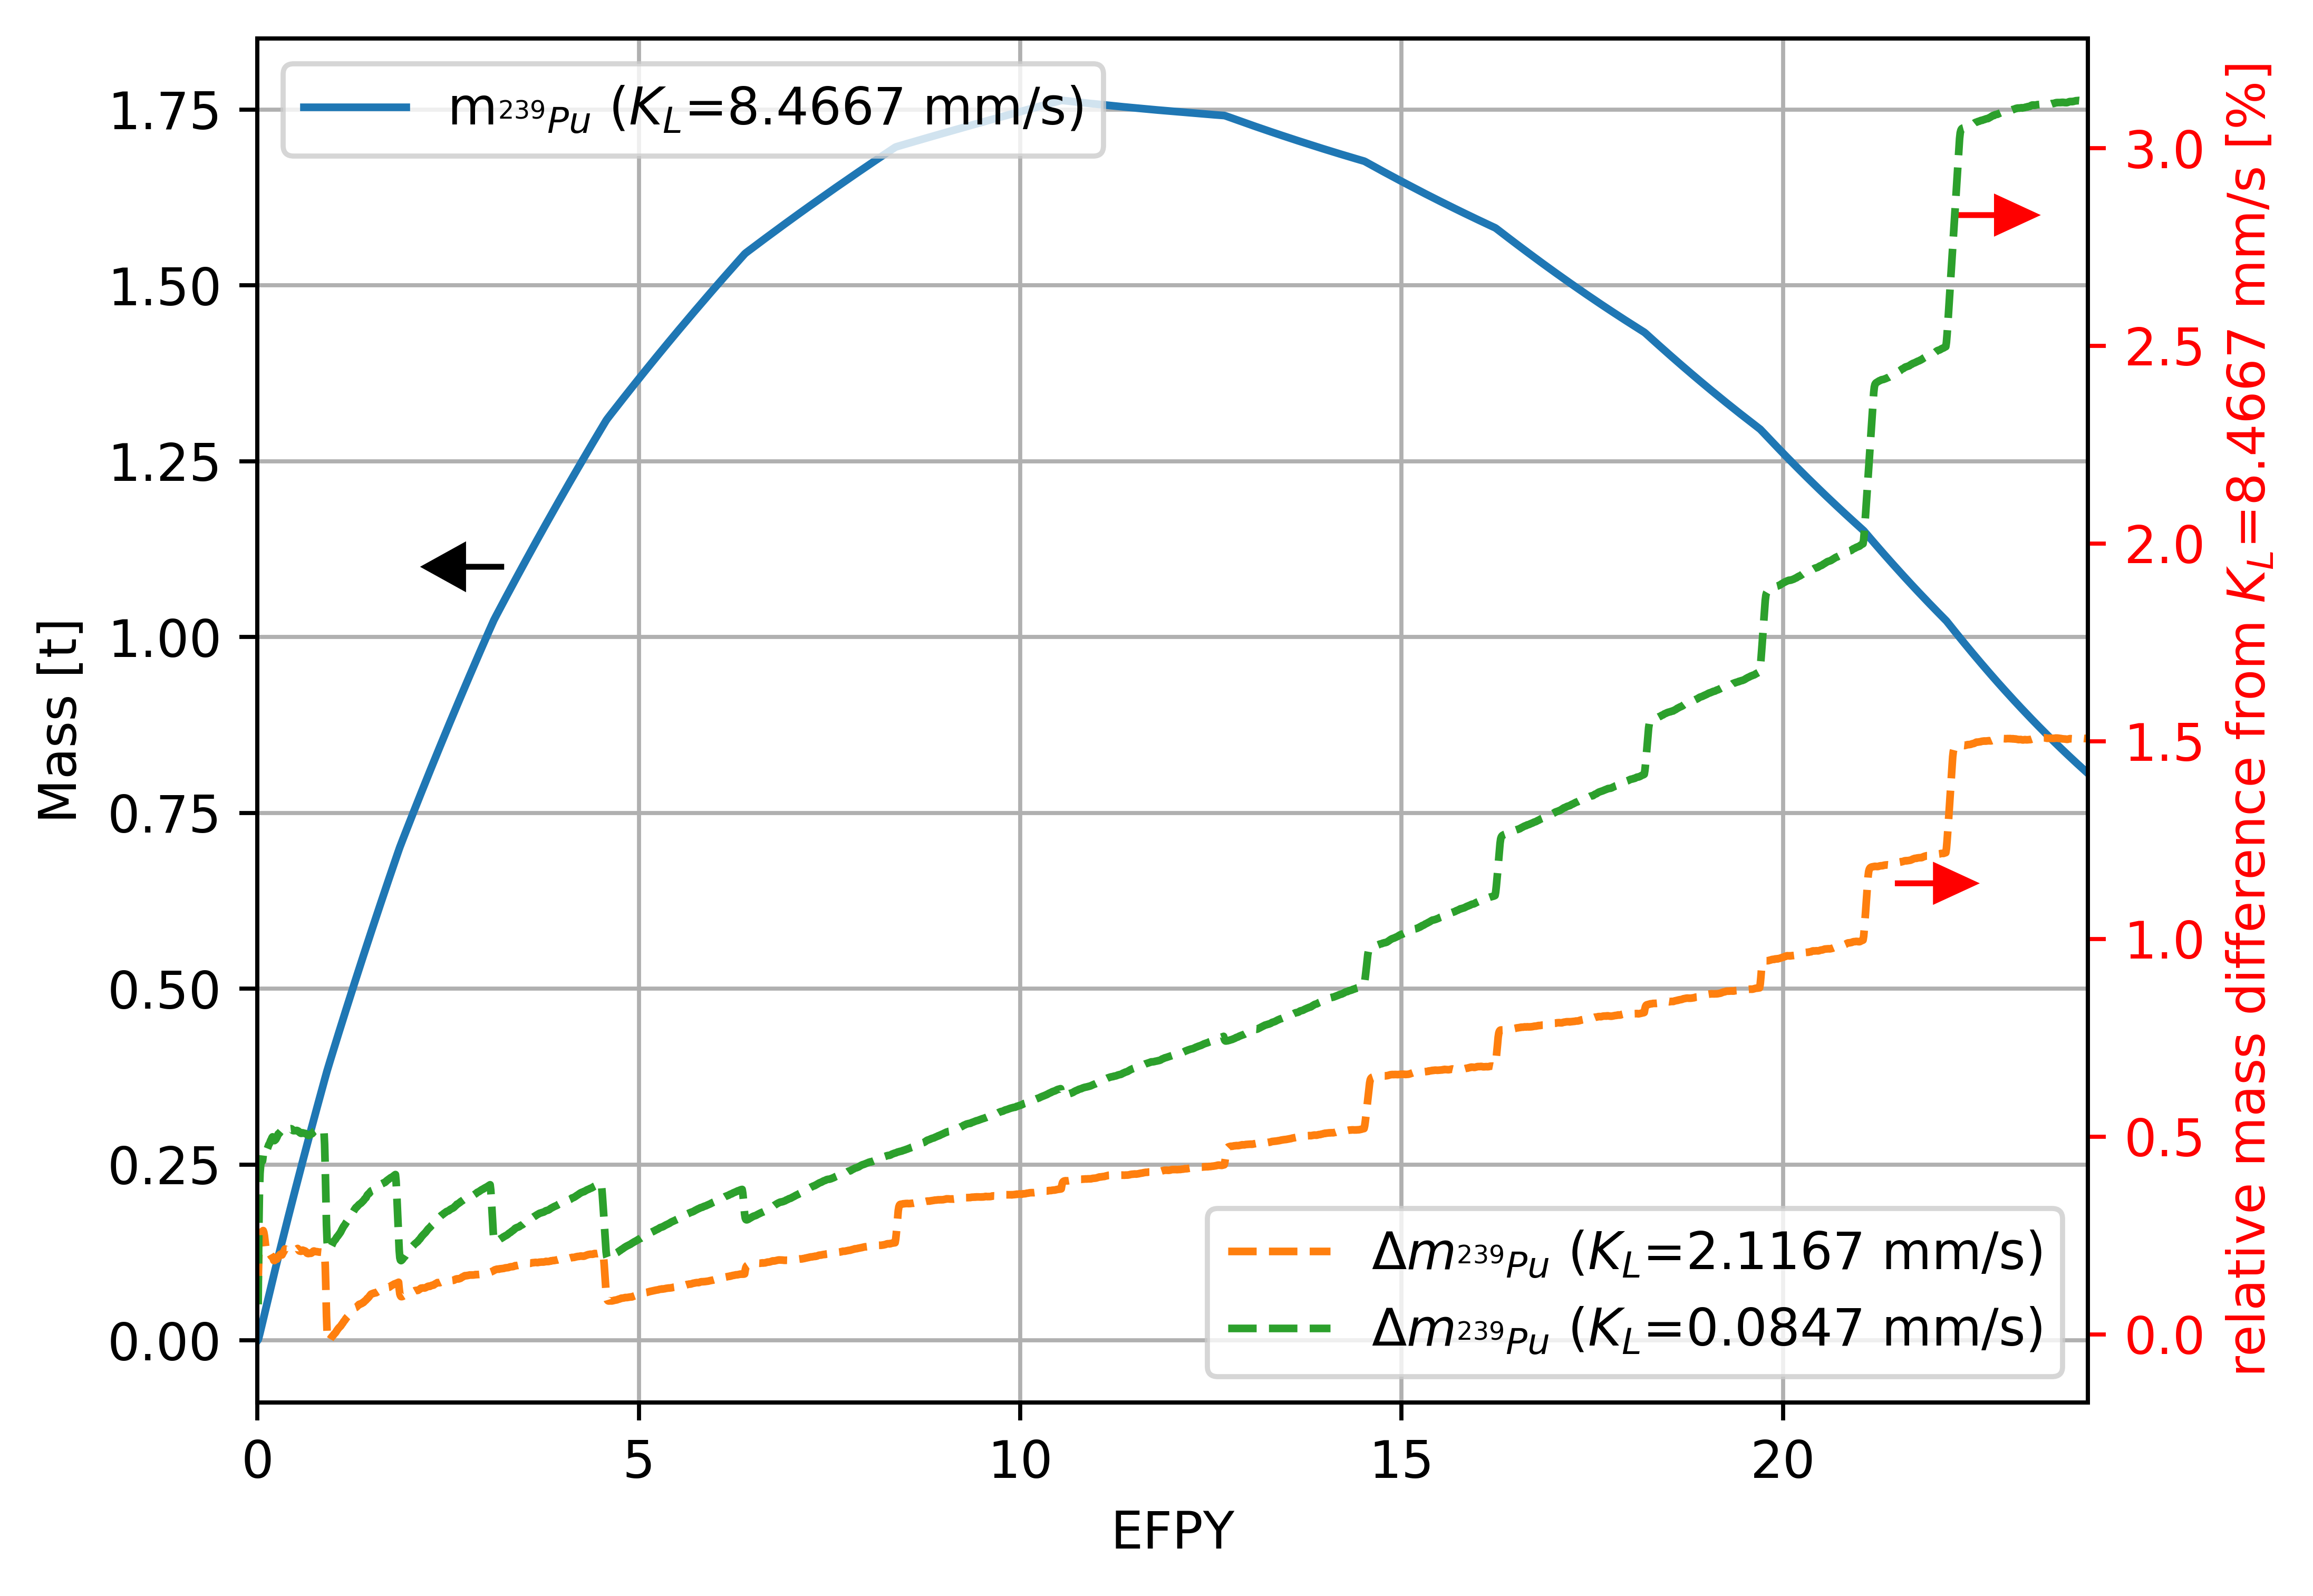
\includegraphics[width=0.77\textwidth]{../dissertation/figures/ch4/eps/pu239.png}
		\vspace{-1mm}
		\caption{SaltProc-calculated mass of $^{239}$Pu in the fuel salt 
		during 25 years of operation for K$_L$ = 8.4667 mm/s compared with 
		less effective noble gas removal.}
	\end{figure}
\end{textblock*}
\end{frame}


\begin{frame}
\frametitle{Impact of xenon poisoning on fuel cycle performance}
\begin{textblock*}{12.4cm}(0.07cm,2.1cm) % {block width} (coords)
	\begin{columns}
		\column[t]{5.5cm}
		\vspace{-5mm}
		\visible<2->
		{\begin{figure}[hbp!] % replace 't' with 'b' to 
			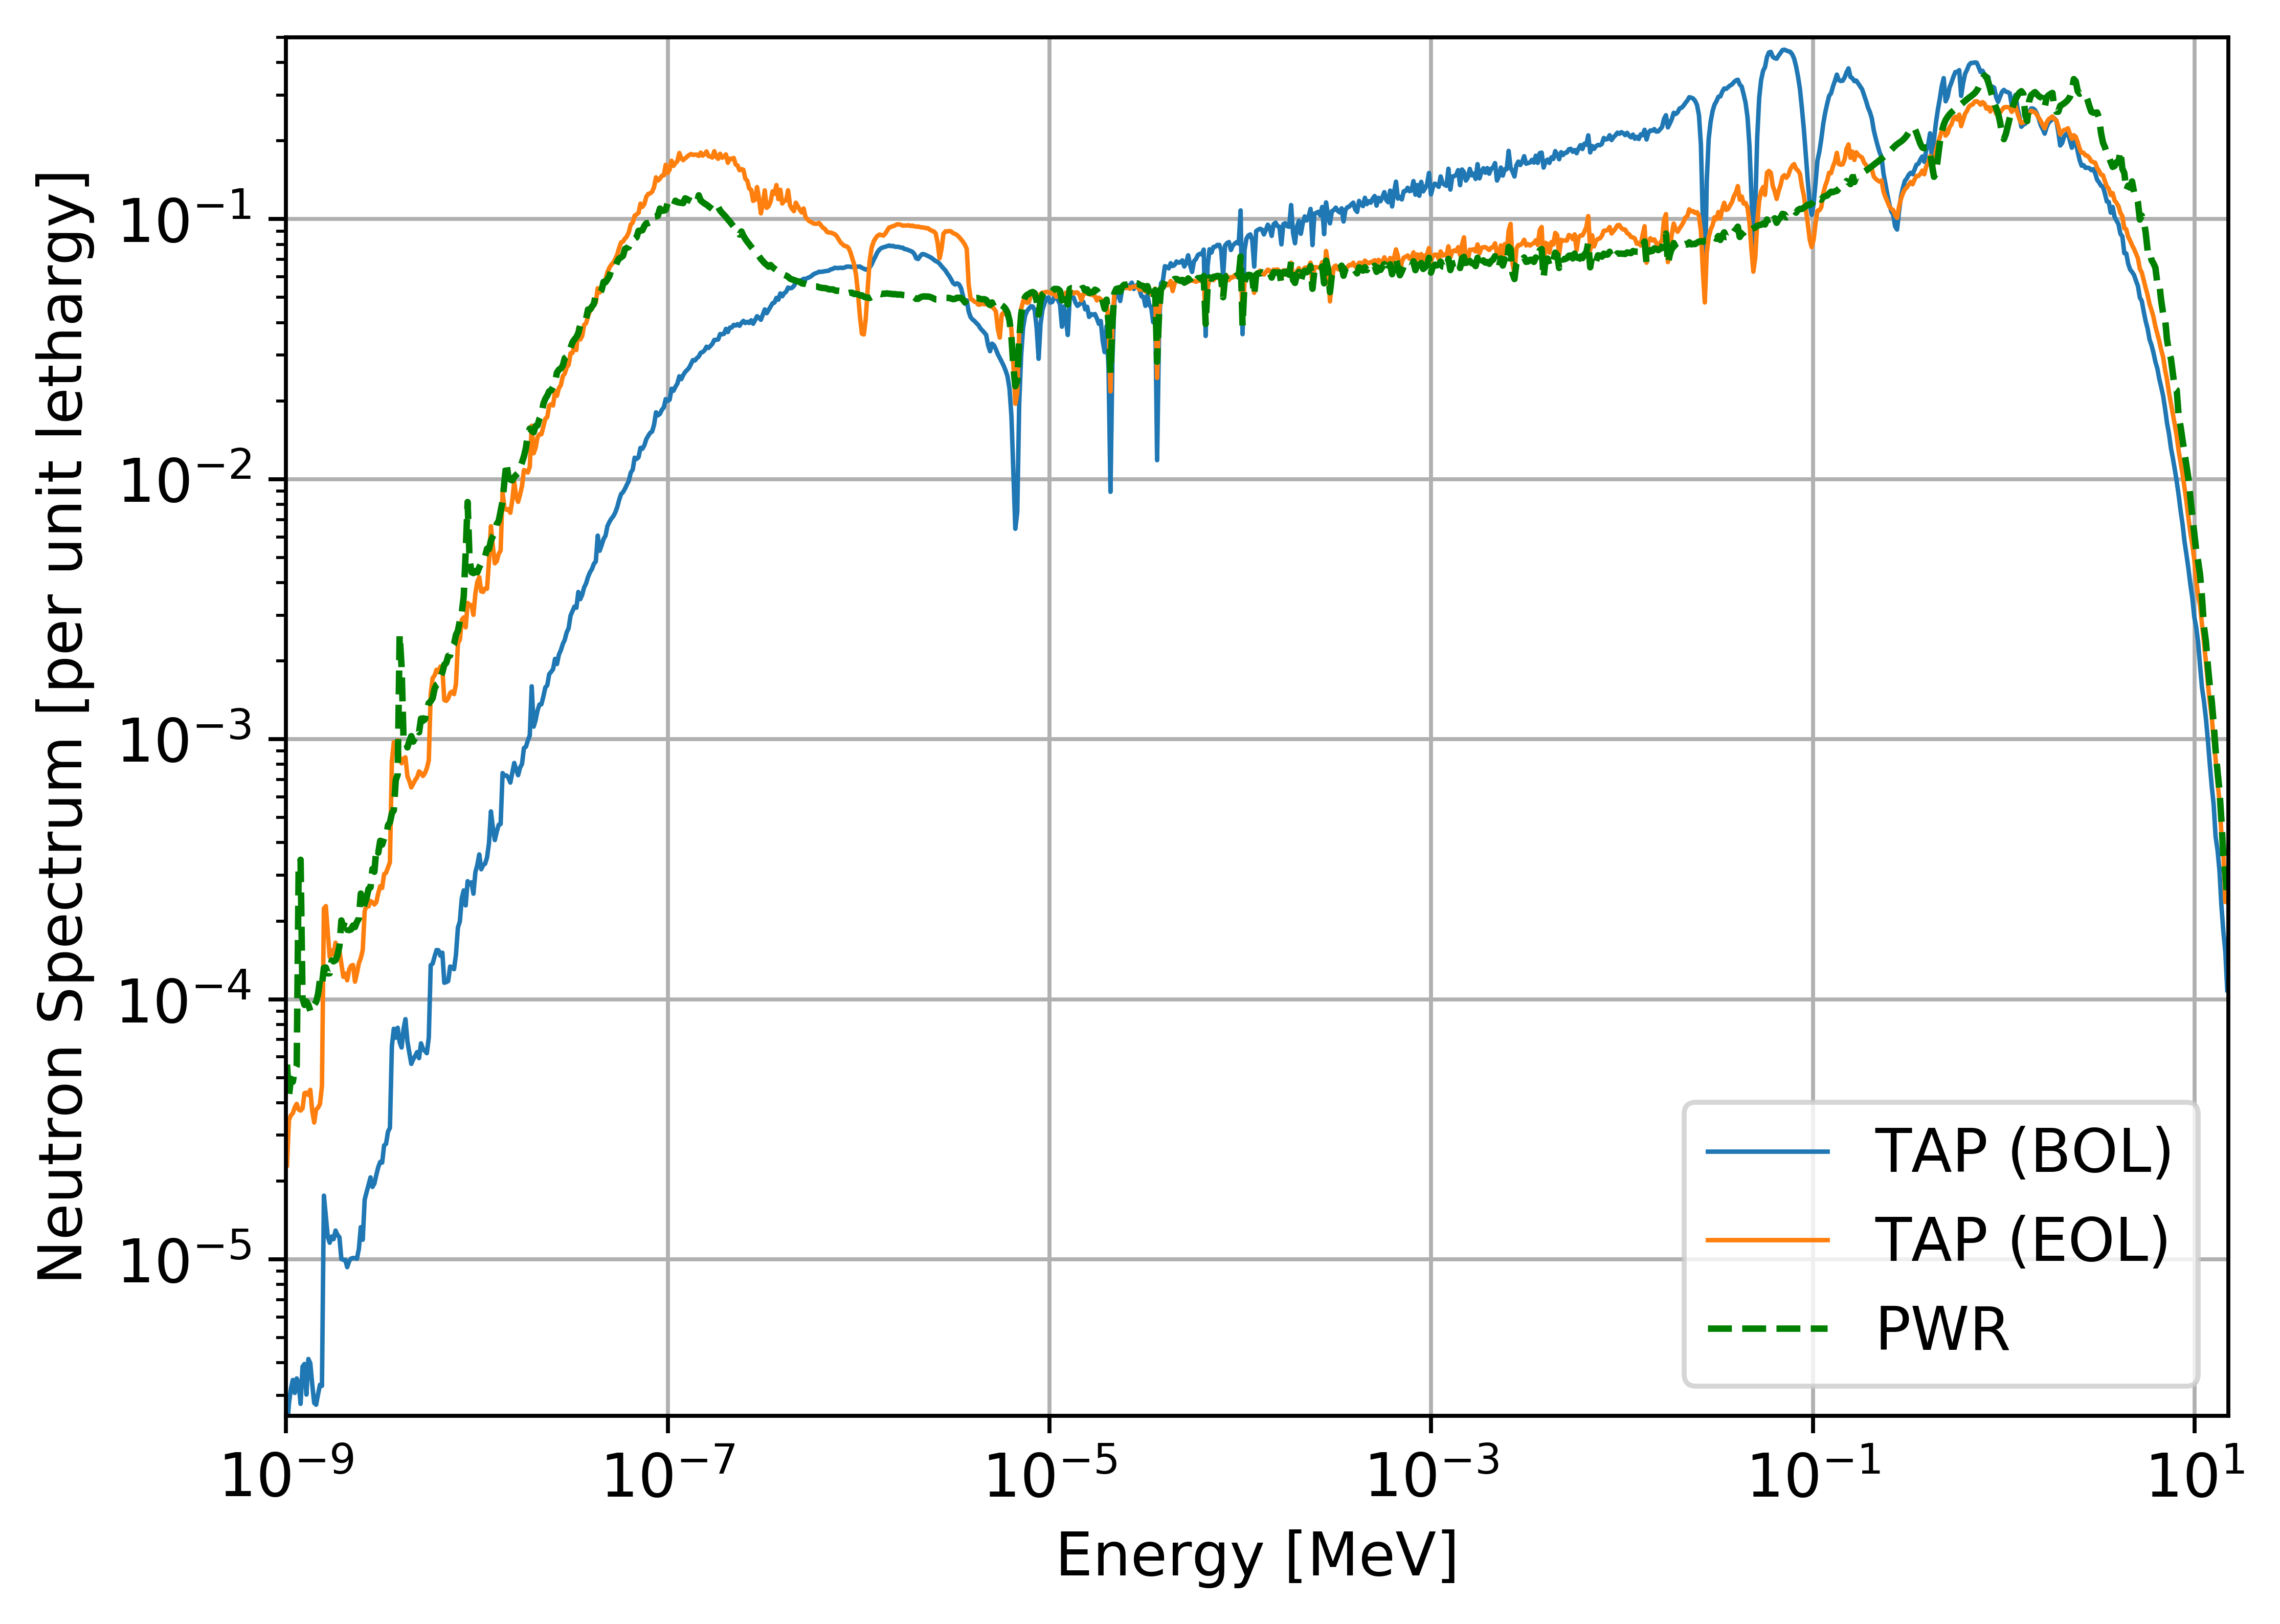
\includegraphics[width=0.94\textwidth]{../dissertation/figures/ch5/tap_vs_pwr_spectrum_2.png}\\
			\vspace{-5mm}
			\hspace{+0.05mm}
			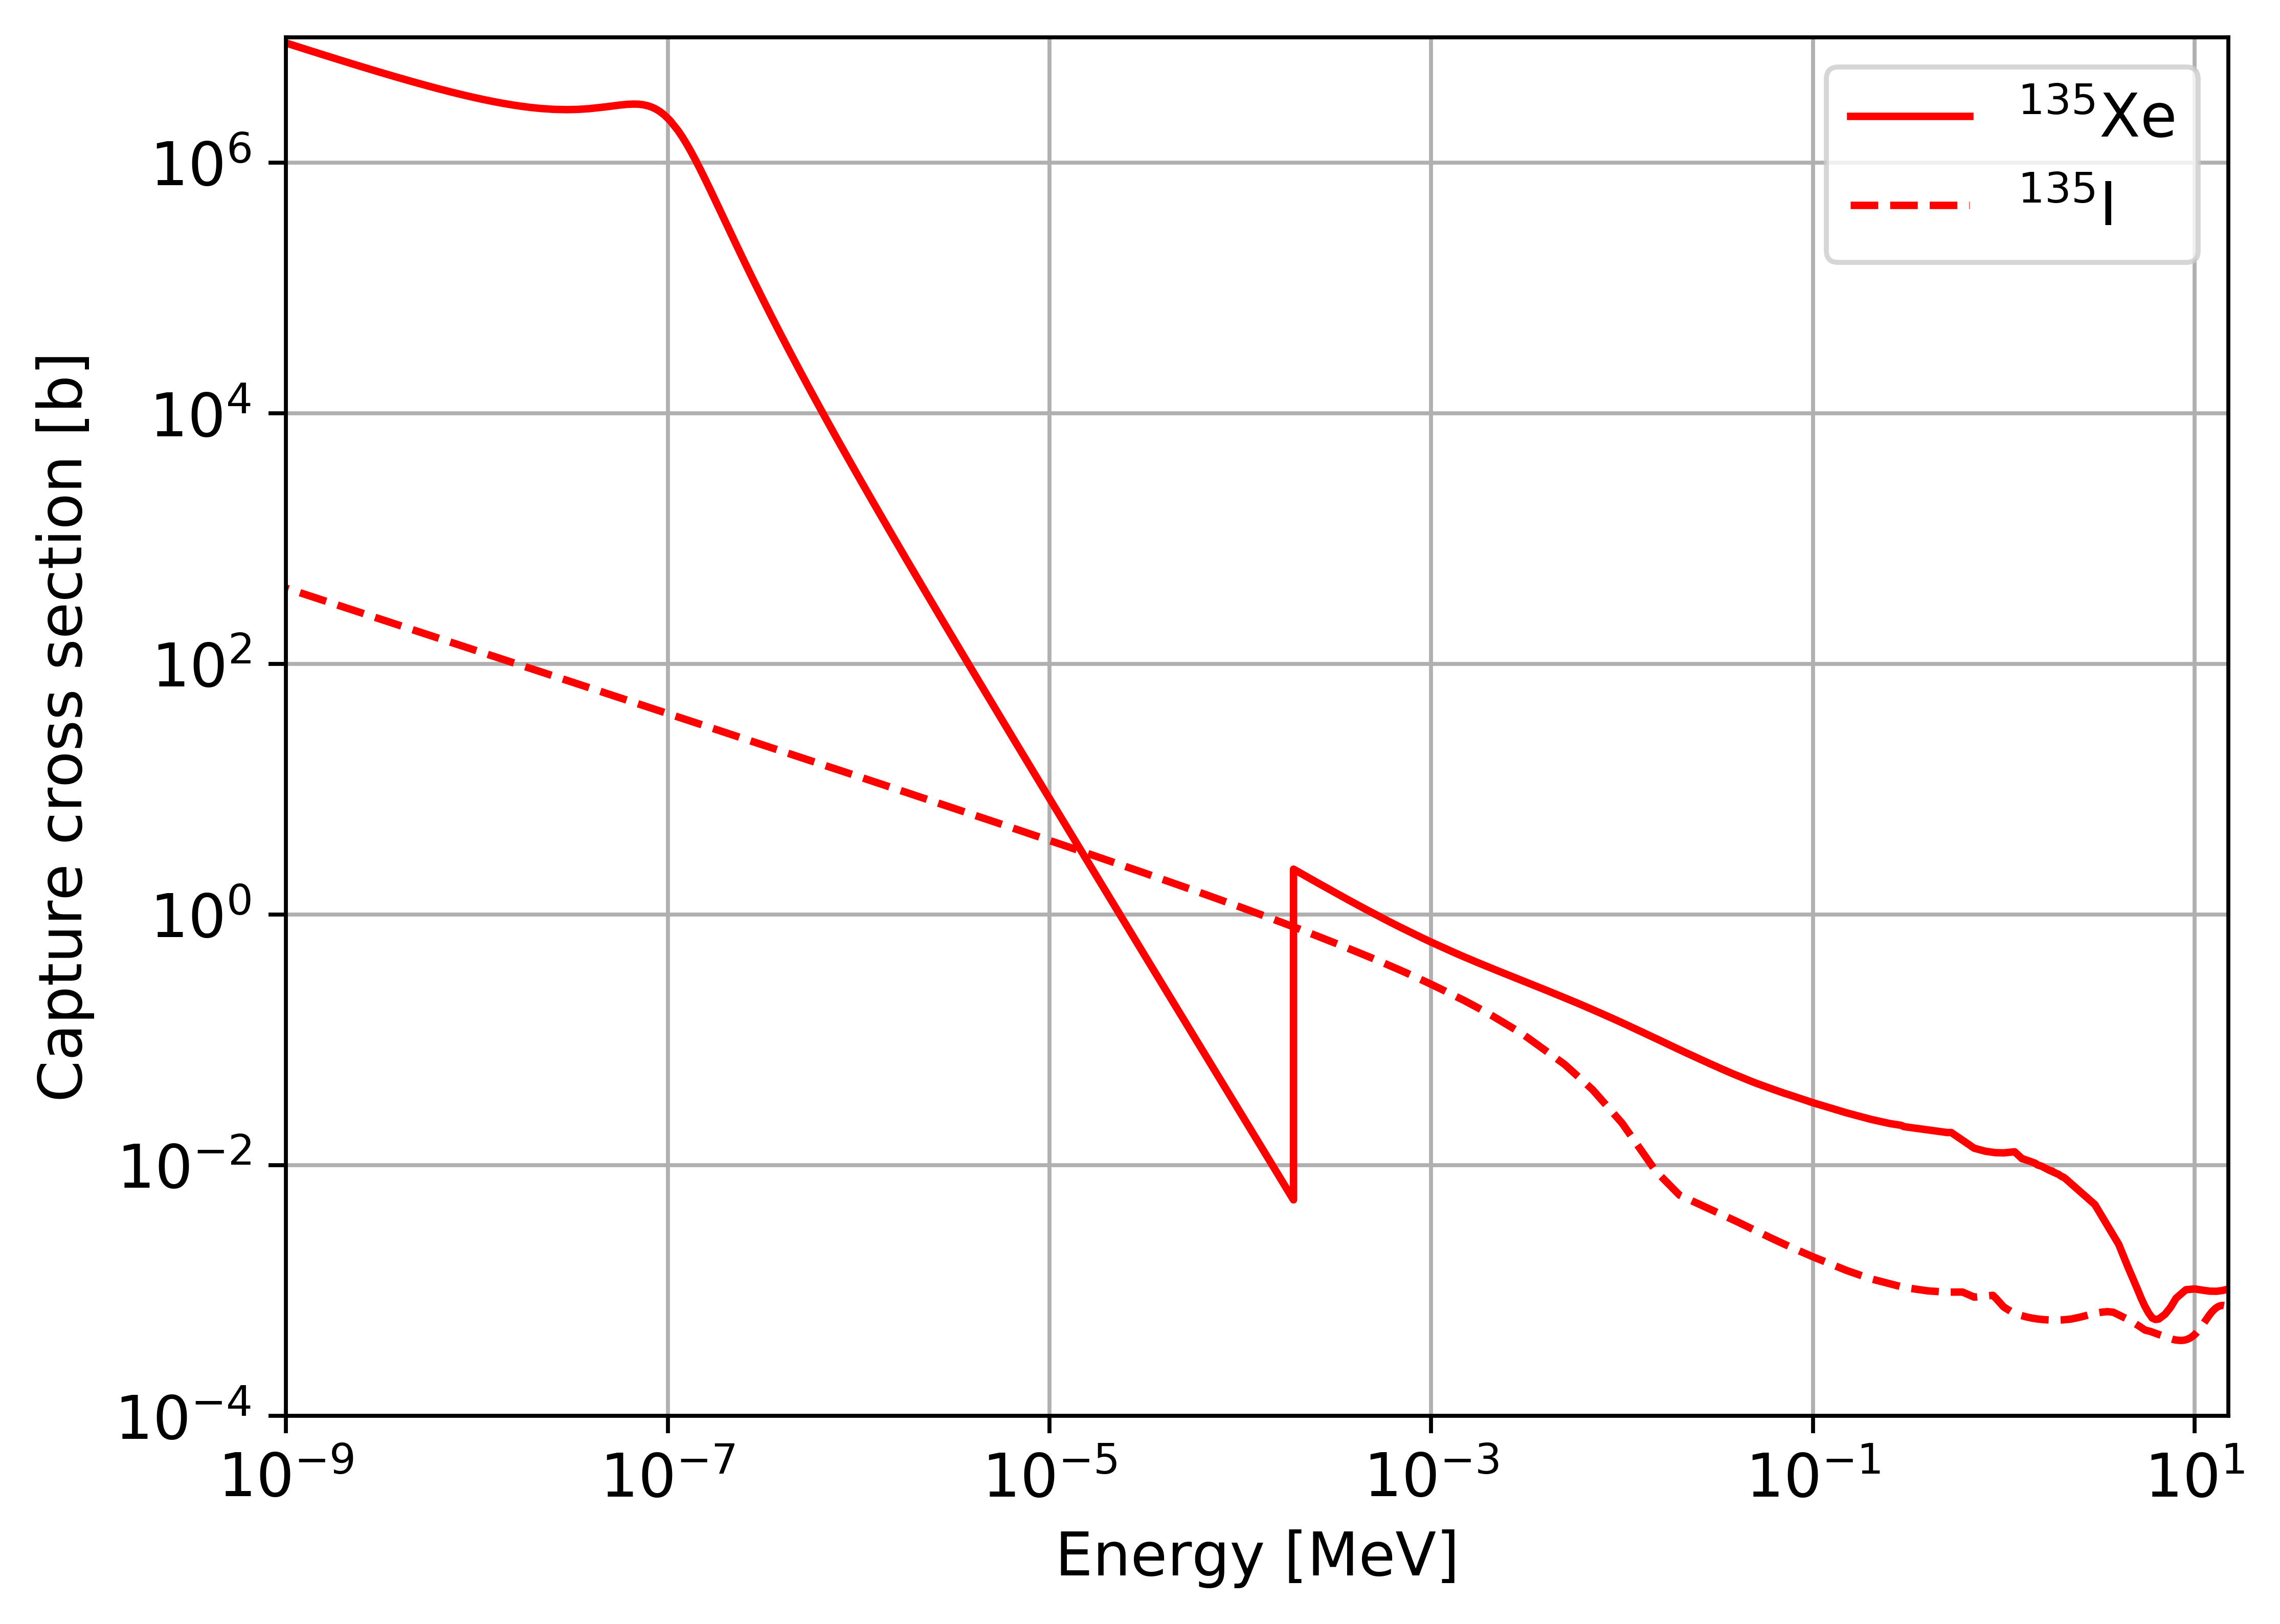
\includegraphics[width=0.94\textwidth]{../dissertation/figures/ch5/i_xe_xs.png}
			\vspace{-3mm}
			\caption{Neutron spectra (upper) and $^{135}$I, $^{135}$Xe caption 
			cross section (lower) \cite{rykhlevskii_impact_2019}.}
		\end{figure}}
		
		\column[t]{6cm}
		\begin{textblock*}{7.3cm}(5.6cm,2.1cm) % {block width} (coords)
		\begin{itemize}
			\itemsep=1em
			\item<1-> \textbf{Less effective} gas removal leads to 
			\textbf{harder} 
			spectrum
			\begin{itemize}
				\itemsep=0.5em
				\item Shorter lifetime due to parasitic absorption
				\item Lower $^{235}$U fission rate
				\item Faster rate of $^{238}$U destruction (-50kg)
				\item Increased breeding of fissile Pu
			\end{itemize}
			
			\item<2-> TAP spectrum \textbf{softens toward EOL}
			\begin{itemize}
				\itemsep=0.5em
				\item Reduced fissile Pu breeding after 11yrs
				\item $\alpha_T$ weakened 
				from $-1.57$ to $-0.26pcm/K$
				\item 12\% CRW degradation
				\item 39\% void coefficient of reactivity ($\alpha_V$) 
				degradation
				\item Lower reactor kinetic parameters ($\beta_{eff}$, 
				$\lambda_{eff}$)
			\end{itemize} 
		\end{itemize}
	
	\visible<3->{\par\small	These observations must be considered during the 
	reactor 
	designing, accident analysis, and safety justification.}
		\end{textblock*}
	
	
	\end{columns}
\end{textblock*}
\end{frame}


\begin{frame}
\frametitle{Uncertainty propagation in depletion calculations (1/2)}
\begin{textblock*}{12.4cm}(0.07cm,1.9cm) % {block width} (coords)
	\begin{columns}
		\column[t]{5.5cm}
		\vspace{-3mm}
		\visible<3->
		{\begin{figure}[hbp!] % replace 't' with 'b' to 
				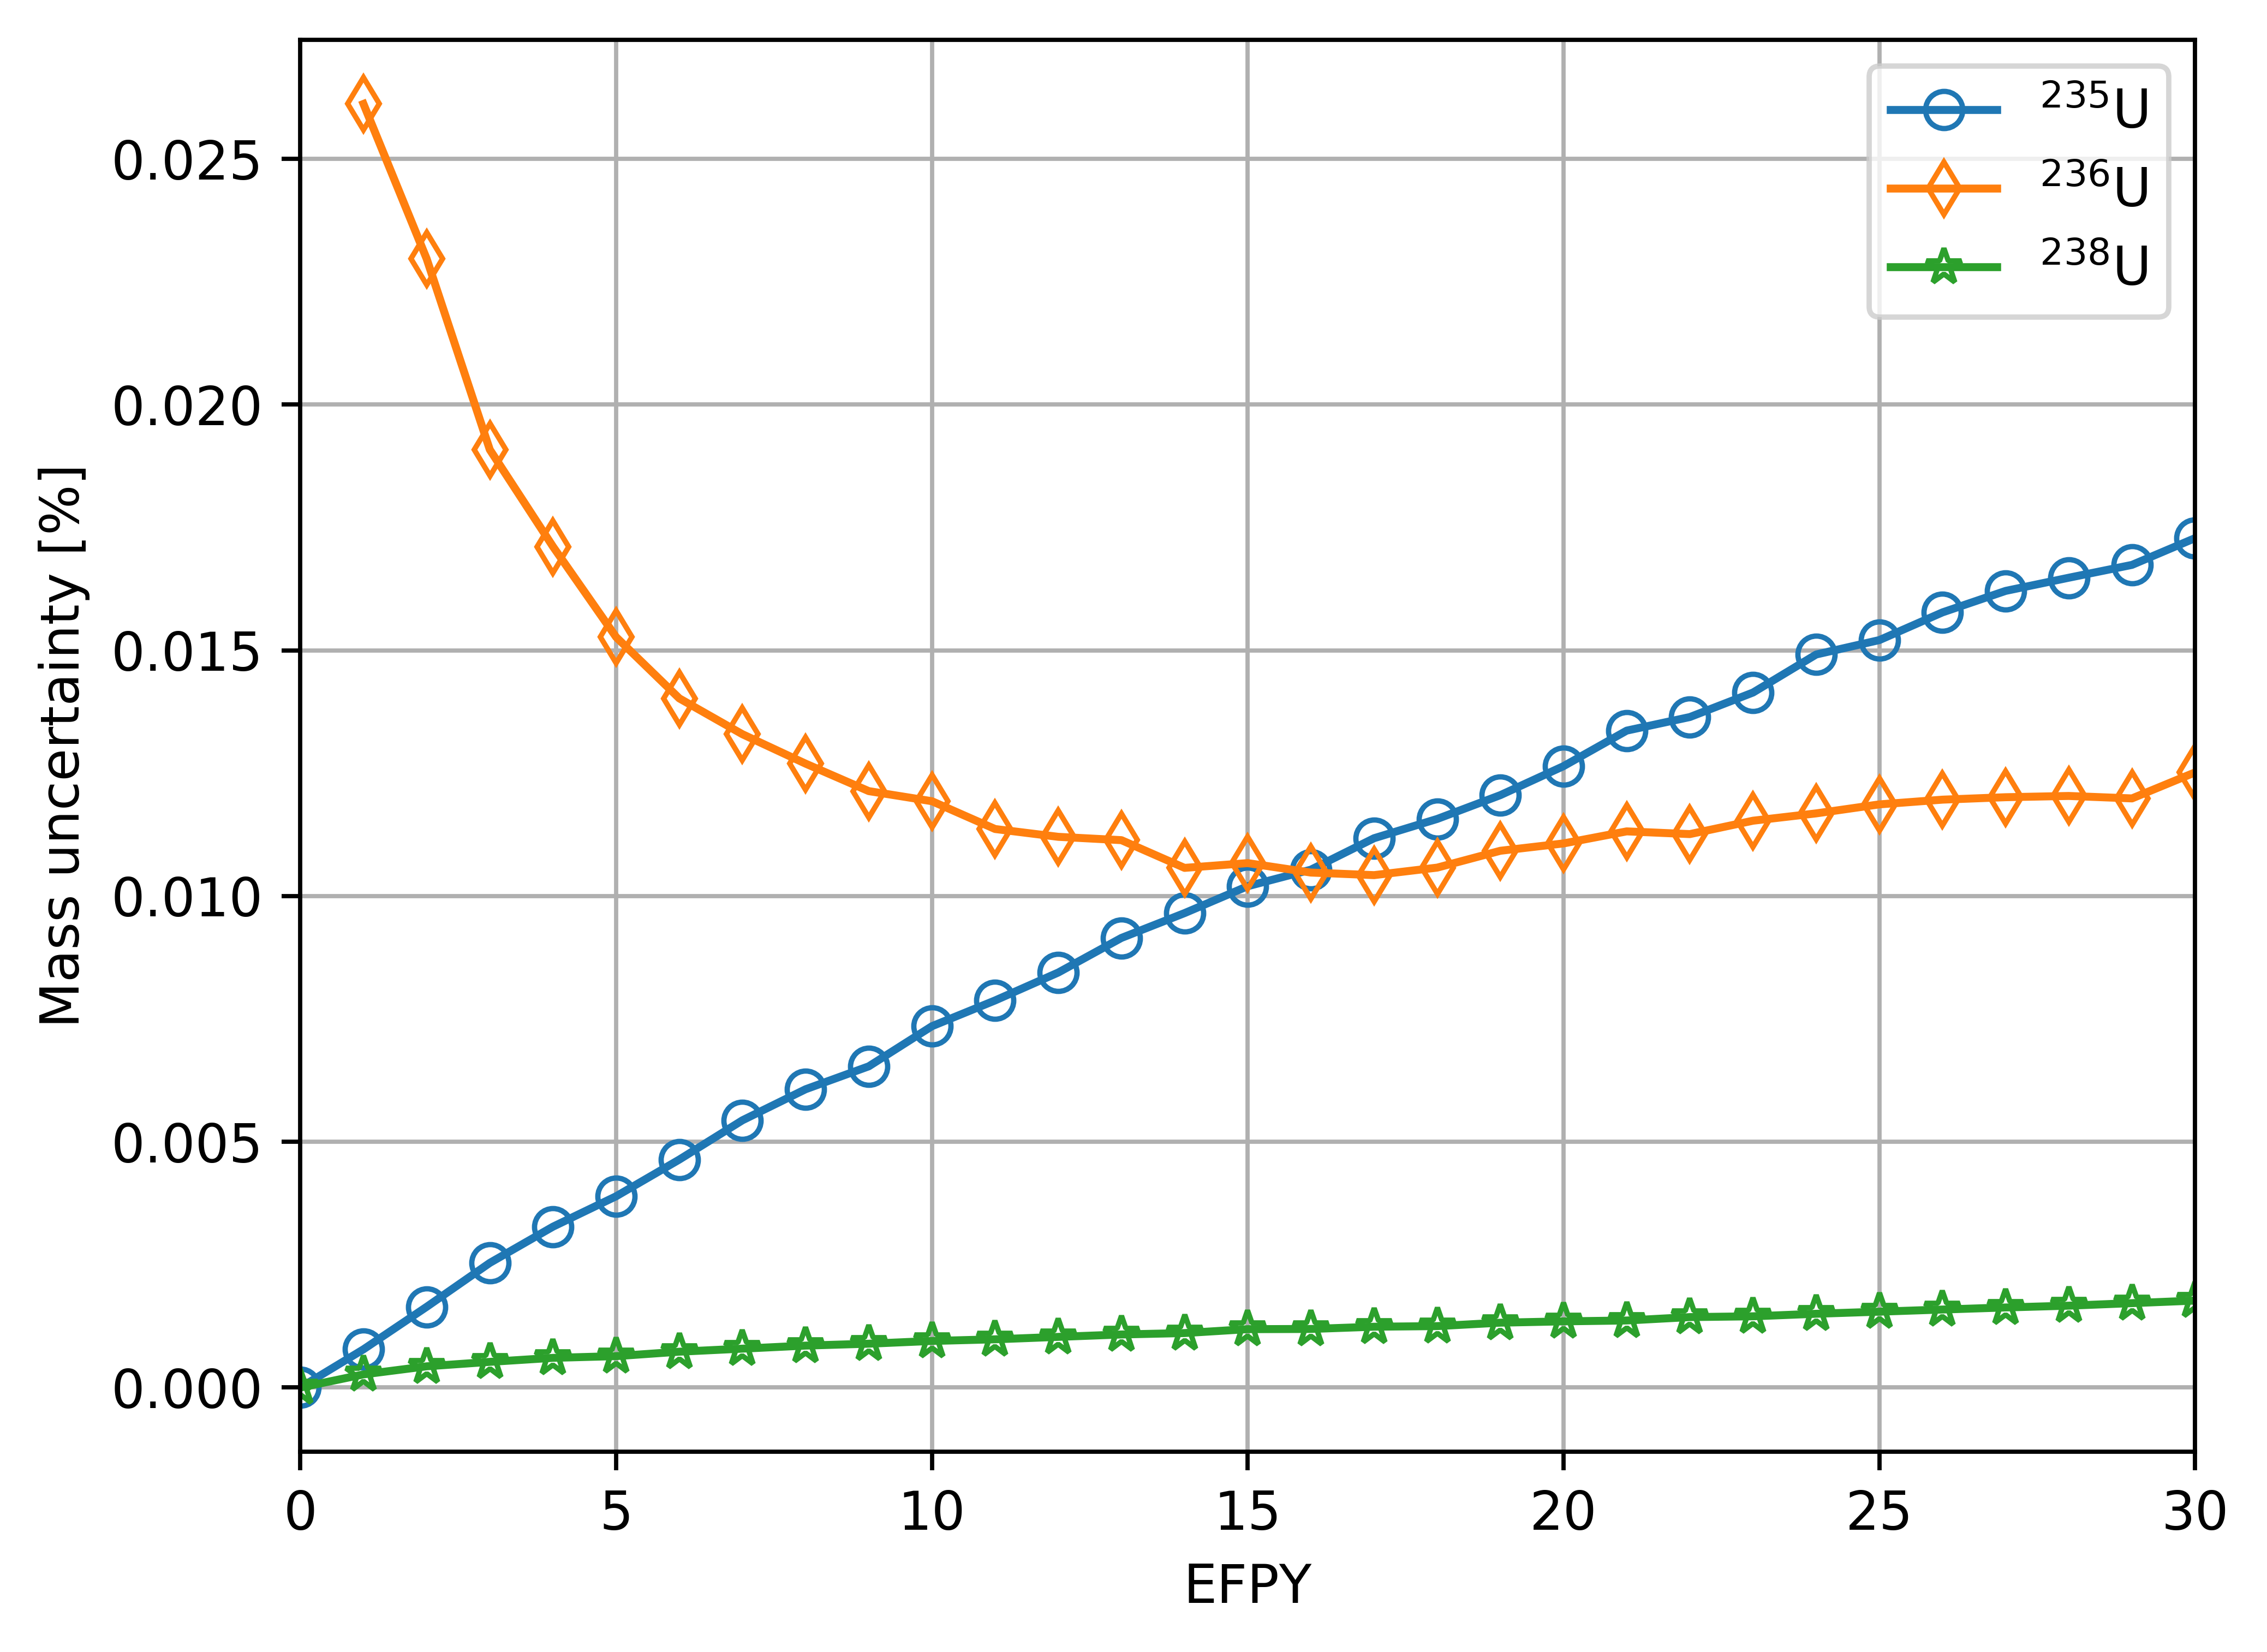
\includegraphics[width=0.92\textwidth]{../dissertation/figures/uq/serpent_mass_std_u.png}\\
				\vspace{-4.5mm}
				\hspace{+0.3mm}
				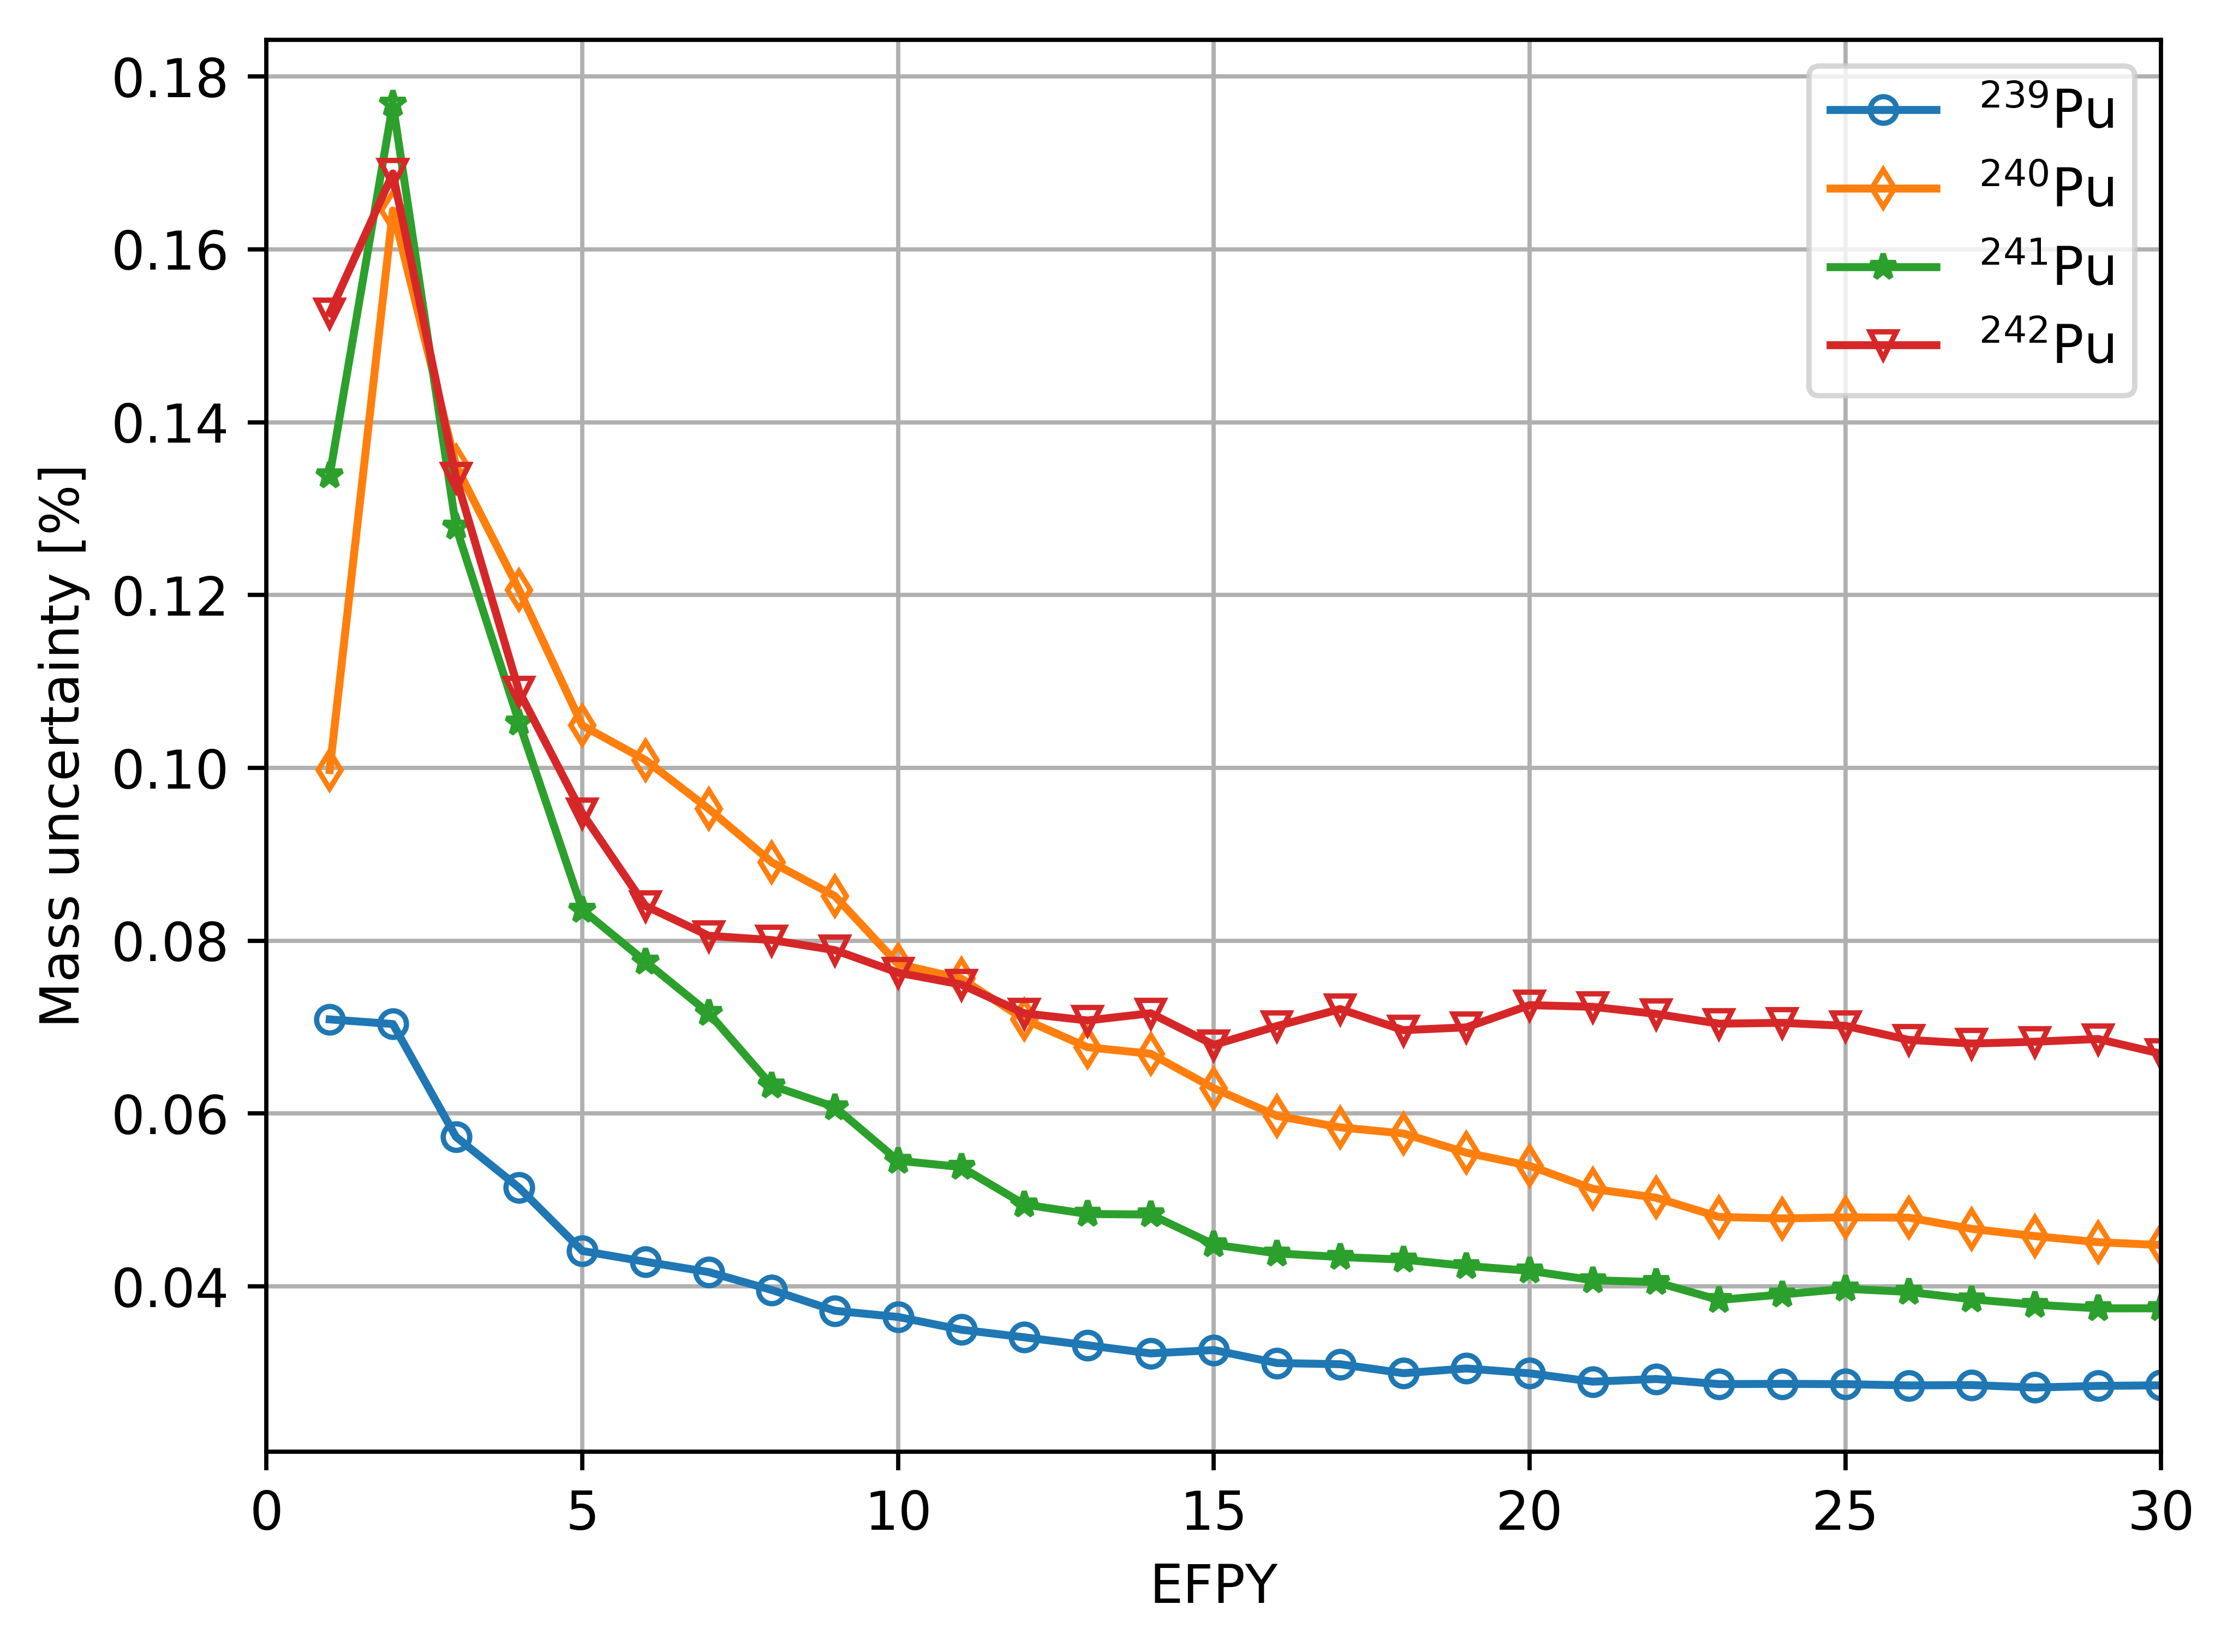
\includegraphics[width=0.91\textwidth]{../dissertation/figures/uq/serpent_mass_std_pu.png}
				\vspace{-3.5mm}
				\caption{Stochastic uncertainty in the uranium and plutonium 
				isotopic inventory.}
		\end{figure}}
		
		\column[t]{6cm}
		\begin{textblock*}{7.2cm}(5.5cm,1.7cm) % {block width} (coords)
			\begin{block}<1->{Sources of uncertainty in depletion calculations}
			\begin{itemize}
				\itemsep=0.3em
				\item<2-> Stochastic uncertainty (Monte Carlo)
				\begin{itemize}
					\itemsep=0.5em
					\item Serpent unable to provide statistical error in 
					predicted composition
					\item Depletion with Serpent \textbf{1000 times, only 
					initial random seed changed}
					\item The mean and standard deviation of isotopic 
					concentration calculated from 1000 samples
				\end{itemize}
				
			\end{itemize}
			\end{block}
			
		\end{textblock*}

	\end{columns}
\end{textblock*}
\end{frame}

\begin{frame}
\frametitle{Uncertainty propagation in depletion calculations (2/2)}
\begin{textblock*}{12.4cm}(0.07cm,1.9cm) % {block width} (coords)
	\begin{columns}
		\column[t]{5.5cm}
		\vspace{-4mm}
		\visible<2->
		{\begin{figure}[hbp!] % replace 't' with 'b' to 
				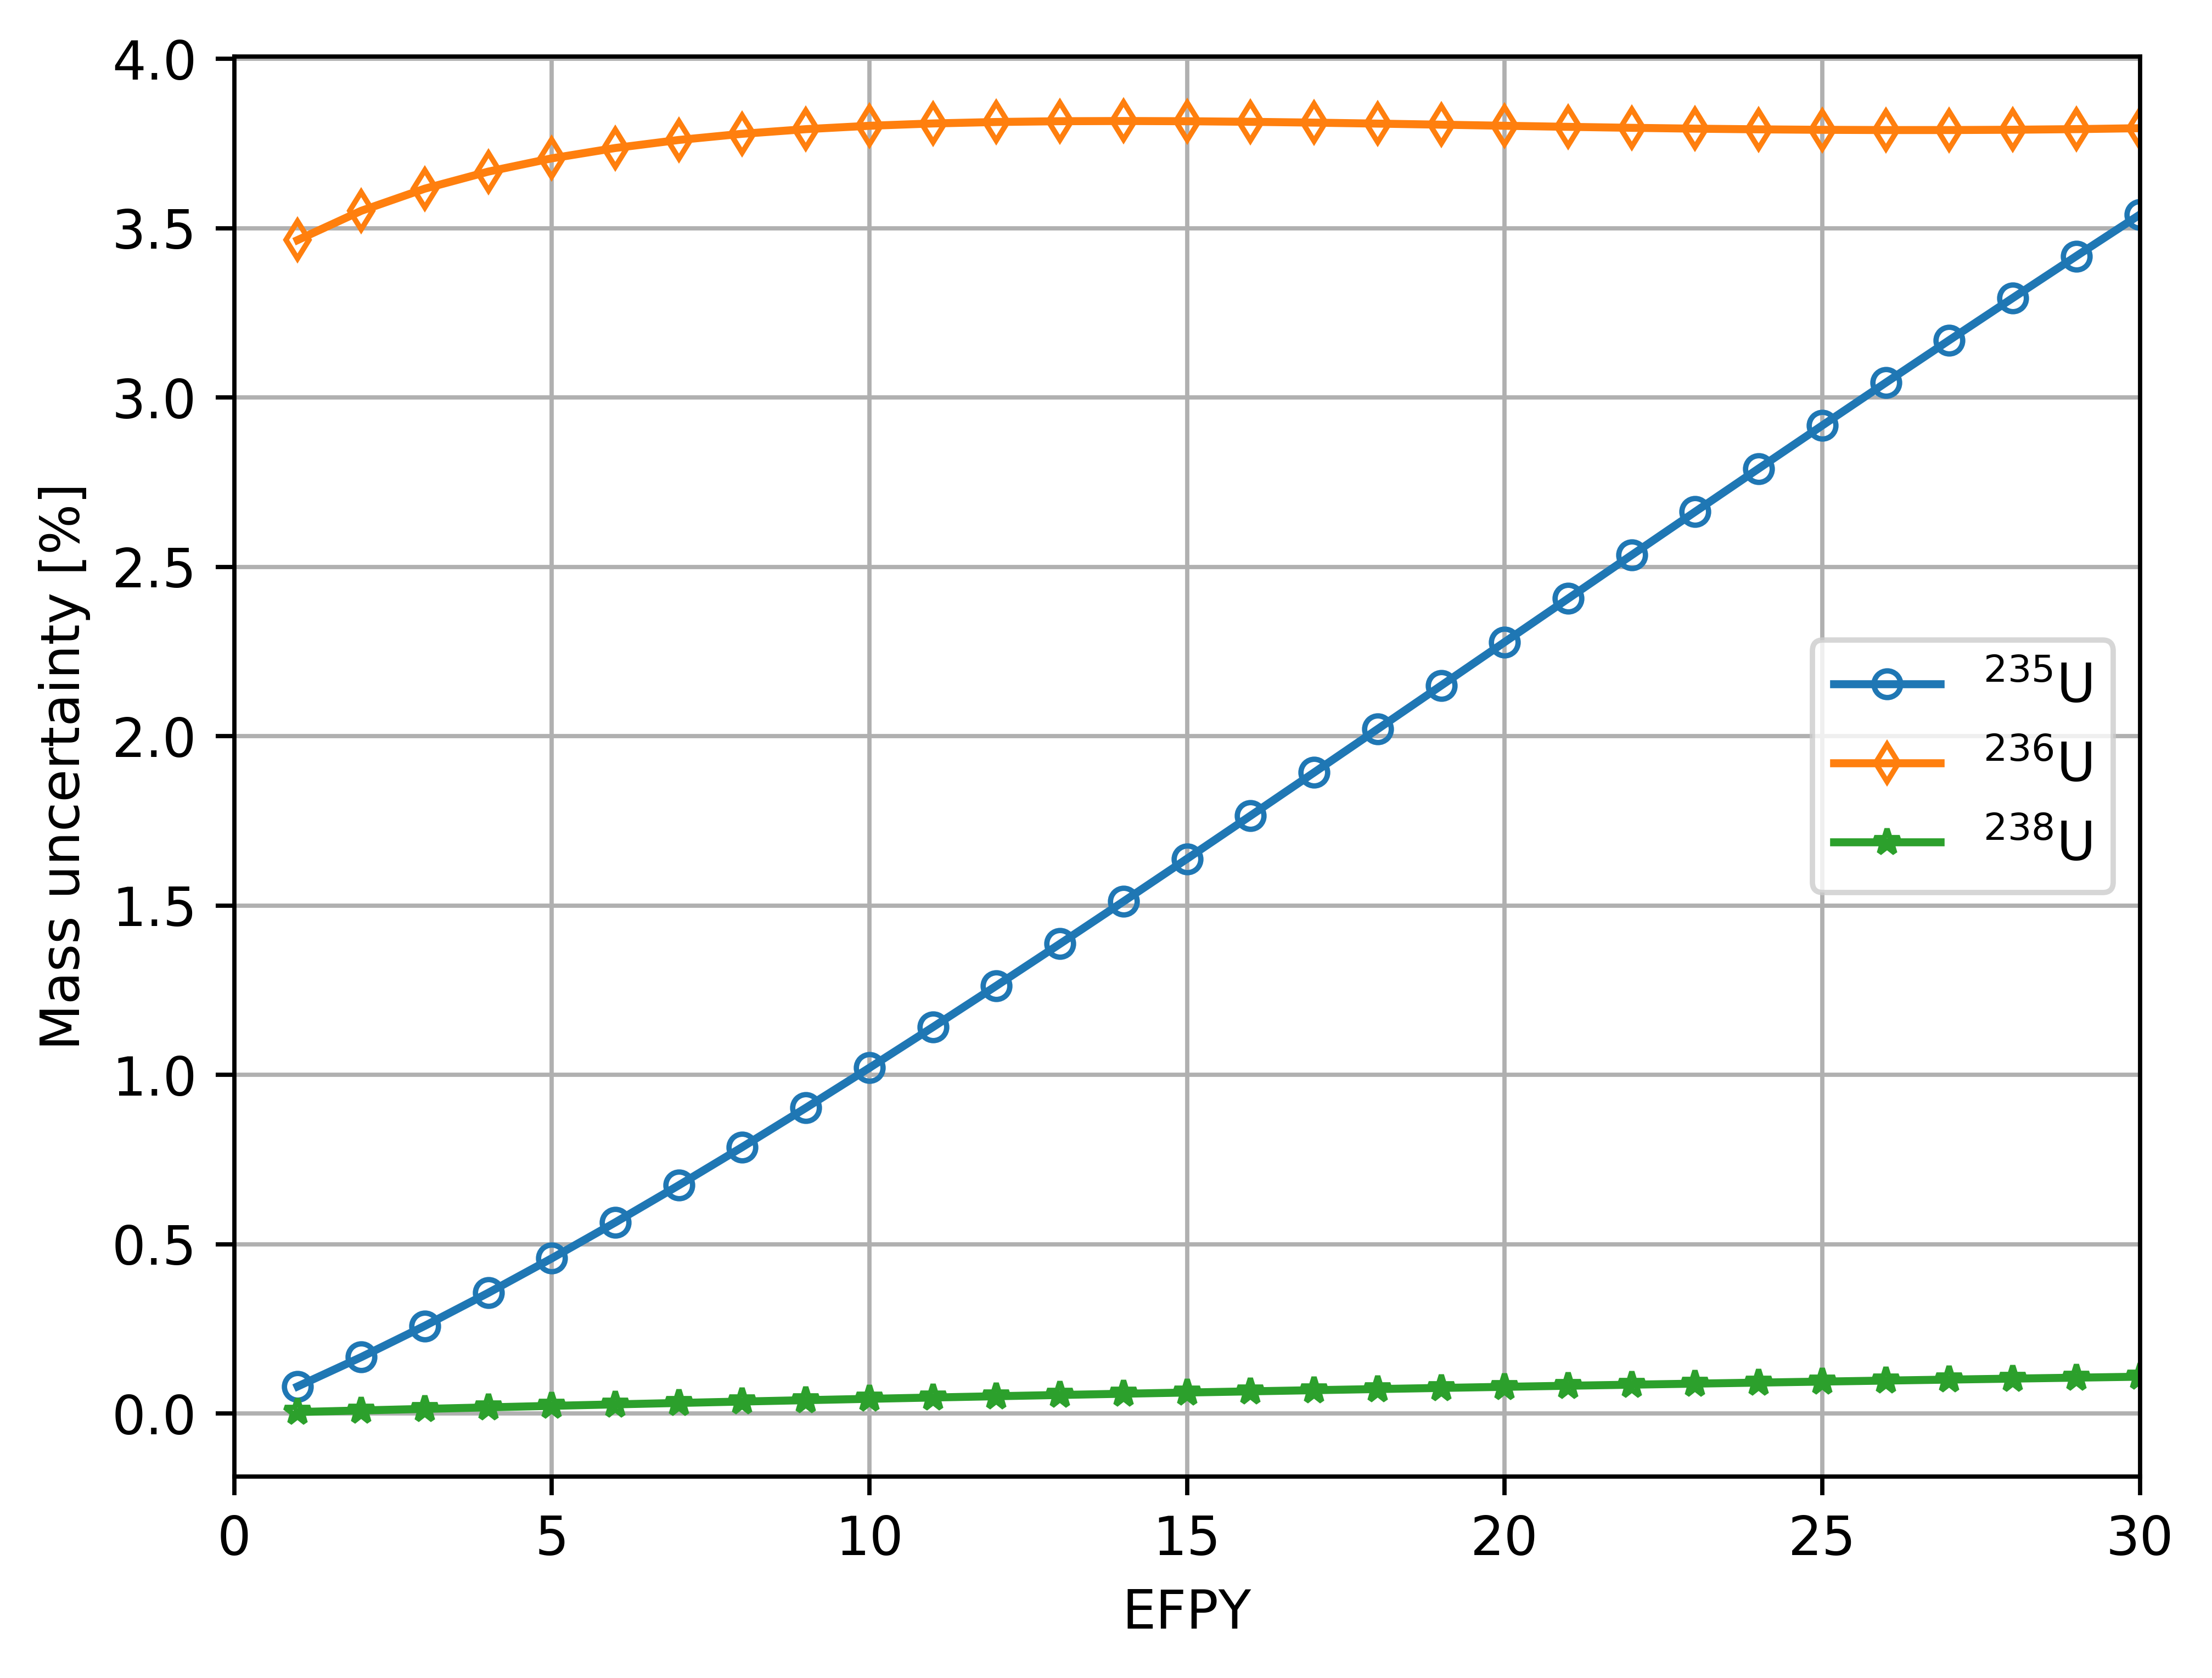
\includegraphics[width=0.9\textwidth]{../dissertation/figures/uq/scale_mass_std_u.png}\\
				\vspace{-4.5mm}
				\hspace{+0.1mm}
				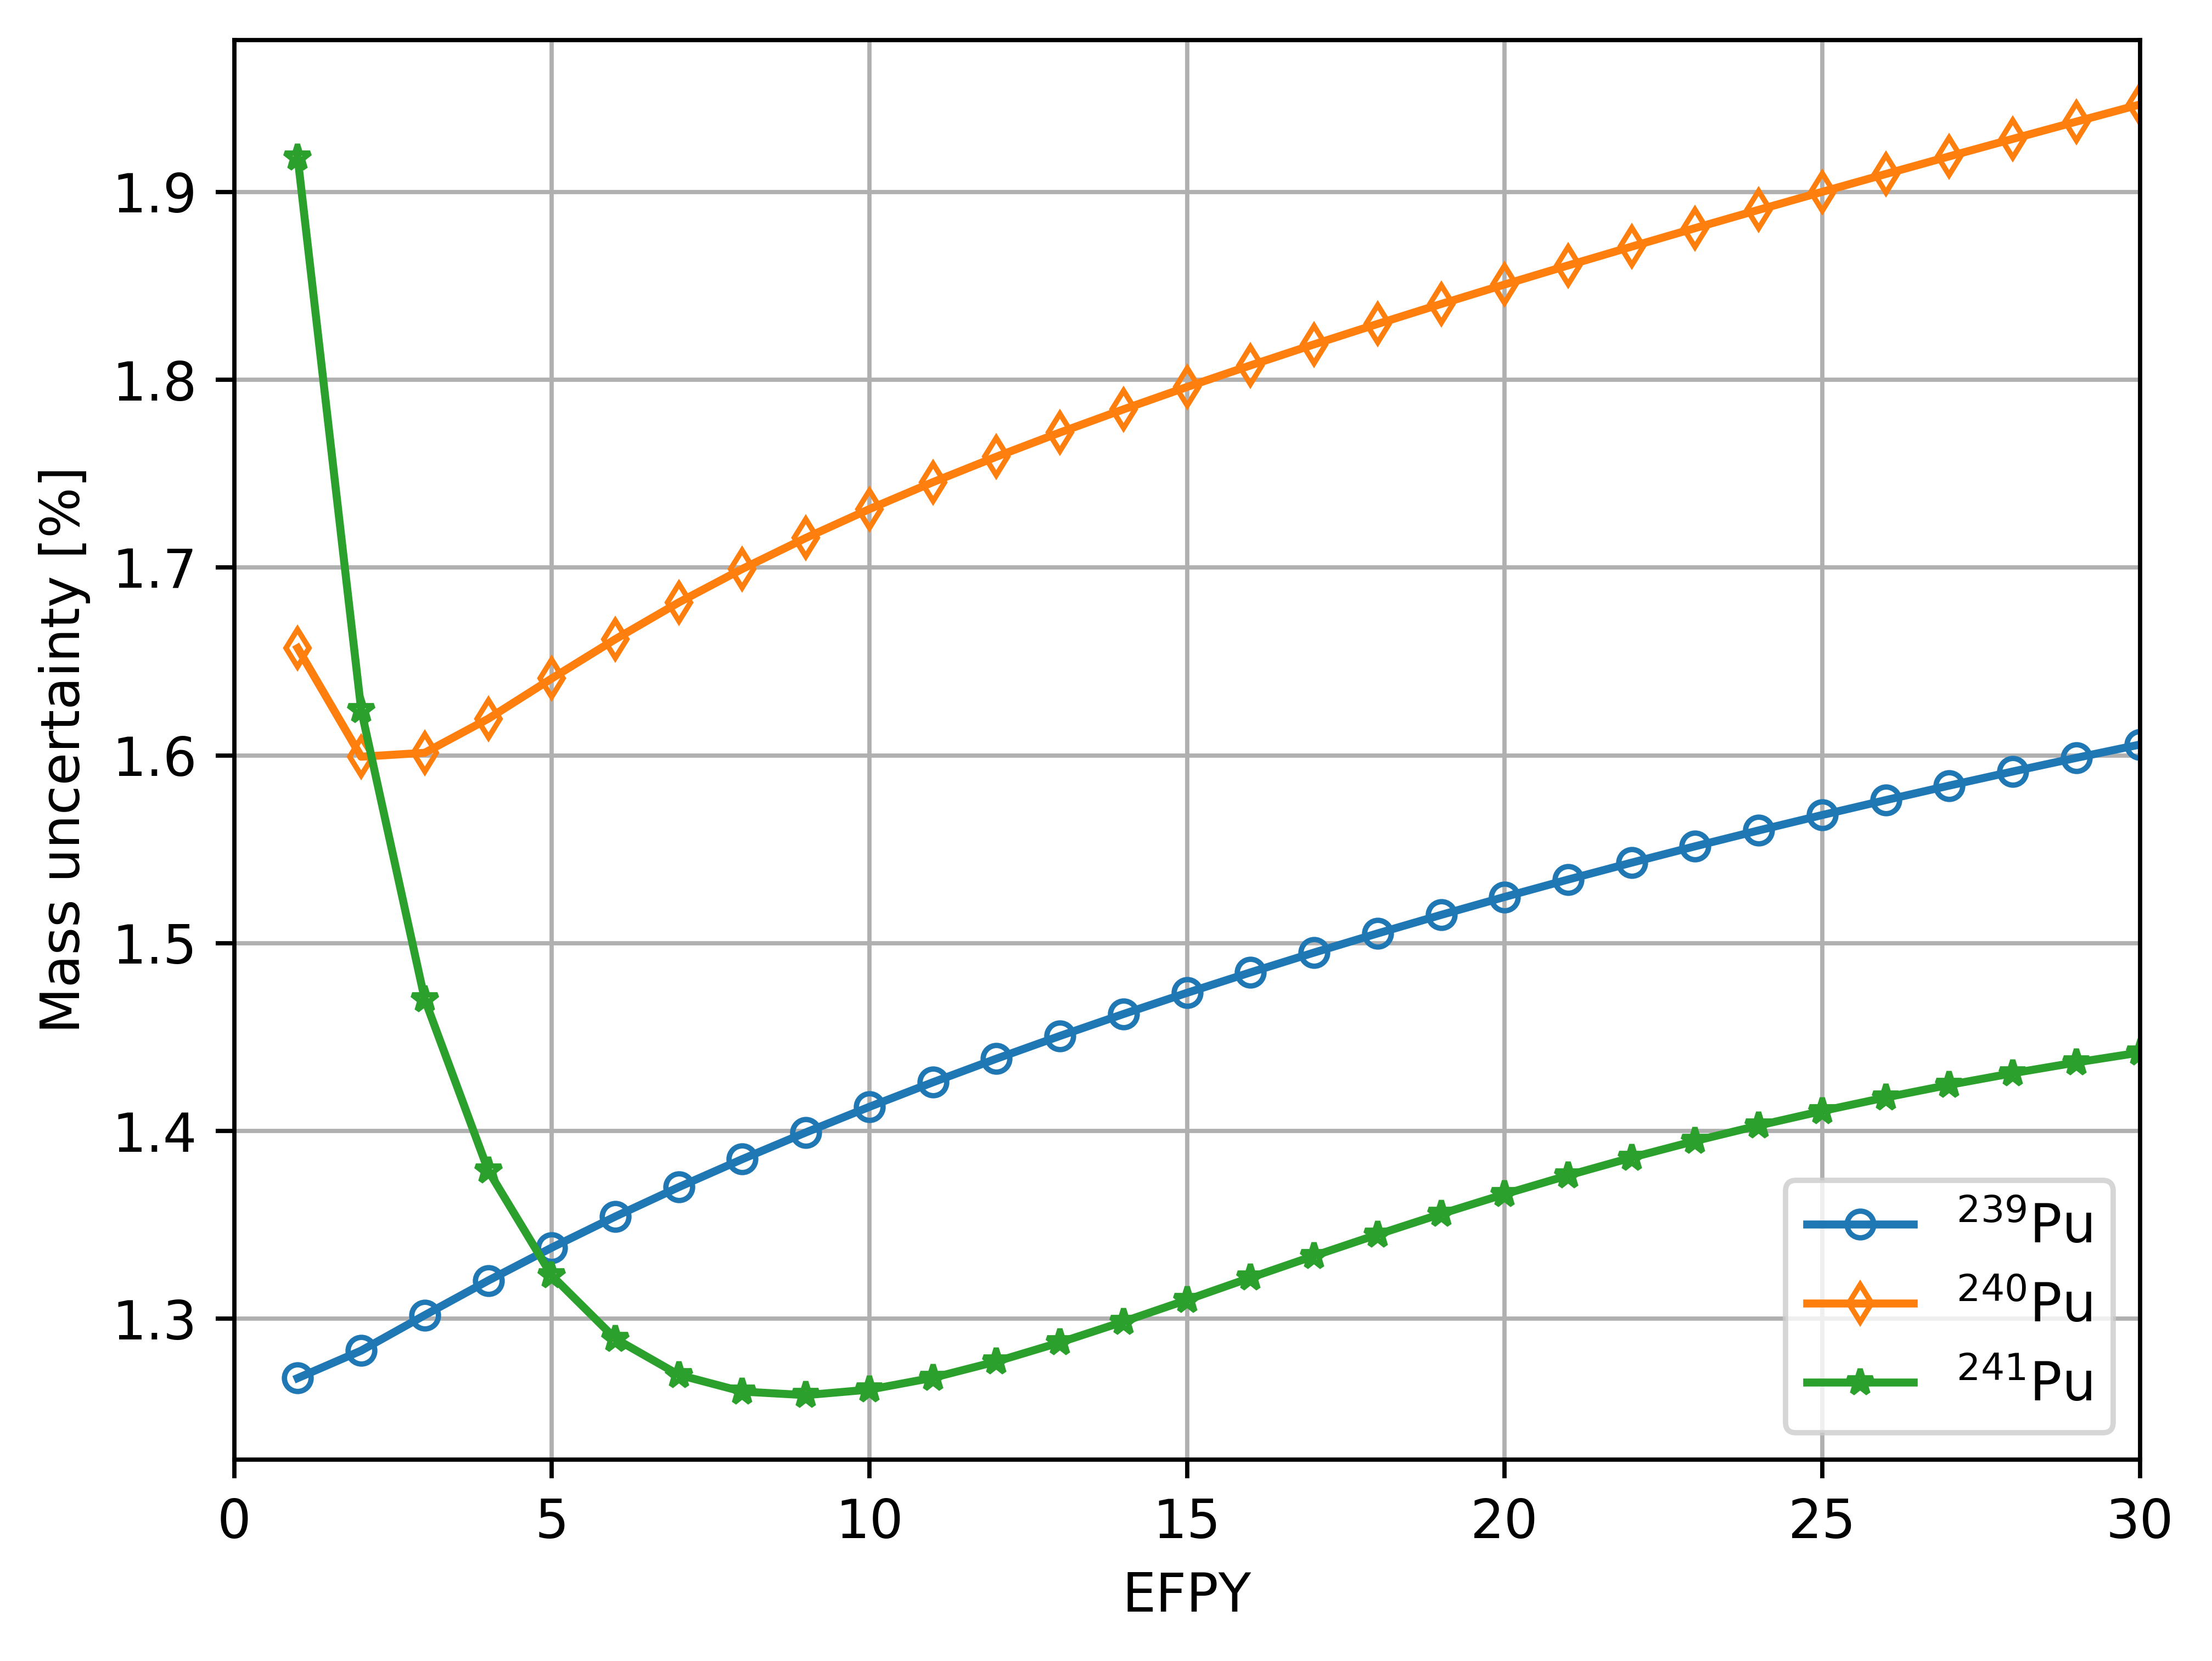
\includegraphics[width=0.9\textwidth]{../dissertation/figures/uq/scale_mass_std_pu.png}
				\vspace{-3.5mm}
				\caption{Nuclear data-related uncertainty \newline in U and Pu 
				isotopic 
				inventory.}
		\end{figure}}
		
		\column[t]{6cm}
		\begin{textblock*}{7.2cm}(5.5cm,1.7cm) % {block width} (coords)
			\begin{block}<1->{Sources of uncertainty in depletion calculations}
				\begin{itemize}
					\itemsep=0.3em
					\item<3> Stochastic uncertainty (Monte Carlo)
					\begin{itemize}
						\itemsep=0.5em
						\item Serpent unable to provide statistical error in 
						predicted composition
						\item Depletion with Serpent \textbf{1000 times, only 
							initial random seed changed}
						\item The mean and standard deviation of isotopic 
						concentration calculated from 1000 samples
					\end{itemize}
					
					\item<1-> Uncertainty in the nuclear data
					\begin{itemize}
						\itemsep=0.5em
						\item Nuclear data covariance propagated via 
						depletion calculations using SCALE Sampler
						\item Simple unit-cell model (NEWT)
						\item Collection of random nuclear data files 
						generated from a multivariate normal distribution and 
						covariances
						\item 800 random samples
					\end{itemize} 
				\end{itemize}
			\end{block}
			\visible<3->{\small \textbf{Takeaway:} Nuclear-data related 
			uncertainty $\times100$ 
			greater that 
			stochastic}
				
		\end{textblock*}
		
	\end{columns}
\end{textblock*}
\end{frame}